\documentclass[10pt]{handout}
\usepackage{amsmath}
\usepackage{enumerate}
\usepackage[parfill]{parskip}
\usepackage{listings}
\usepackage{enumitem}
\usepackage{tikz}
\usepackage{graphicx}
\usepackage[lofdepth,lotdepth]{subfig}
\usepackage{multicol}
\usetikzlibrary{shapes,arrows}
\tikzset{node distance=5cm}
\tikzstyle{block} = [rectangle, draw,%
  text width=5em, text centered, rounded corners, minimum height=5em]
\tikzstyle{line} = [draw, -latex']
\tikzstyle{cloud} = [draw, ellipse, text centered, minimum height=2em, text
  width=4em]
\tikzstyle{process} = [draw, rectangle, minimum height=3cm, text width = 6cm,
  dashed]

\lstset{basicstyle=\footnotesize\ttfamily,language=Python,escapeinside=\$\$,
  showstringspaces=false}

\author{
  Allen Chen, \emph{allenchen@berkeley.edu}\\
  Jon Ko, \emph{jonathan.ko@berkeley.edu}\\
  Young Kim, \emph{y.kim@berkeley.edu}\\
}
\course{Computer Science 194-16}
\semester{Spring 2012}

\runningtitle{SICP}
\title{Starcraft 2 International Competition Predictor}

\begin{document}
\maketitle

\section{Introduction}
What's the biggest e-sport in the world? Ask anyone, and there's only one answer: Starcraft 2. Compared to other video games, Starcraft 2 undisputedly holds the title of the most popular and funded competitive scene. But, with all these big names like MVP or MMA going around, this brings up the question: who is the best? Better yet, can we figure out what factors are indicators on who would win a match? As avid fans of Starcraft 2, these are questions we aim to answer in this project in the hopes that not only will we discover who is the undisputed king but also how to improve our own game.

\section{Data Scraping}
\subsection{teamliquid}
We obtain our data from \href{http://www.teamliquid.net/tlpd/sc2-international/games}{teamliquid's match result listings} for both the Starcraft II International and Korean sections. Their site provides such high level details for each match as the date played, map name and internal ID, and winner and loser name, internal ID, and race played. Looking through the site via a browser behaves perfectly fine, but we soon discovered that the site enforces a request rate limit on arbitrary calls (e.g. curl, HTTP libraries). We attempted to contact teamliquid by email to request access to their data, but the short answer was that we'd have to obtain the data ourselves.

\subsection{Implementation}
We implement a scraper script in Ruby that pulls information from the teamliquid site and saves it to CSV locally. The Mechanize and Nokogiri gems allow easy, object-oriented parsing and navigation of the site, and allows us to create a relatively simple yet modular framework for collecting from multiple data sources across the site. We simply input a scraper module (currently only two, for match results or for maps) and the script will cycle through the paginated table, parsing and accumulating the data. When we first wrote the script, there were 1323 pages of results, so we also added parameters to specify start and end pages, in order to parallelize the scrape across multiple Apple Orchard machines. The final dataset of results was just over 4 megabytes in size, plus a small constant-size list of approximately 90 maps.

\subsection{Extracted Data}
We obtain the following fields from match results:
\begin{multicols}{2}
\begin{itemize}
  \item \verb$date$
  \item \verb$league_id$
  \item \verb$league_name$
  \item \verb$map_id$
  \item \verb$map_name$
  \item \verb$winner_id$
  \item \verb$winner_name$
  \item \verb$winner_race$
  \item \verb$loser_id$
  \item \verb$loser_name$
  \item \verb$loser_race$
\end{itemize}
\end{multicols}

We obtain the following fields from the table of maps:
\begin{multicols}{2}
\begin{itemize}
  \item \verb$map_id$
  \item \verb$map_name$
  \item \verb$map_size$
  \item \verb$map_spots$: Number of starting positions
\end{itemize}
\end{multicols}




\section{Data Visualization}
TO-DO: Allen fill this in
\subsection{Background and Goals}
In StarCraft, players can play as one of three different futuristic races: the Protoss, the Terran and the Zerg.  Each one of these races have unique capabilities, and play very differently.  Often times, these racial imbalances can be made apparent by comparing race win rates over time.  With the visualizations, our main goals were to find the highest-performing players with a high confidence and analyze trends in racial imbalance in the game.

\begin{figure}[t]
  \centering
  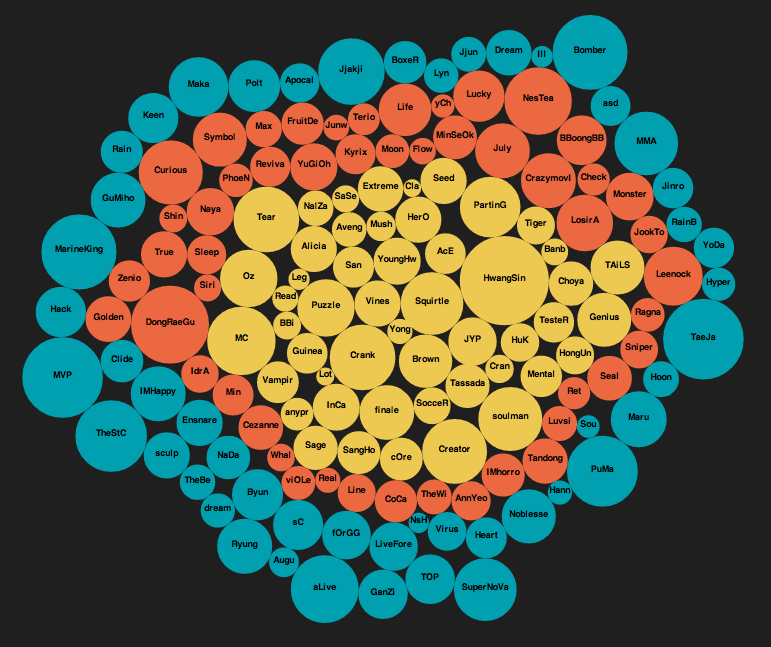
\includegraphics[scale=.35]{pics/bubble_players.png}
  \caption{High-Performing Players - Zerg is Red, Terran is Blue, Protoss is Yellow.  Larger is better.}
\end{figure}
\begin{figure}[t]
  \centering
  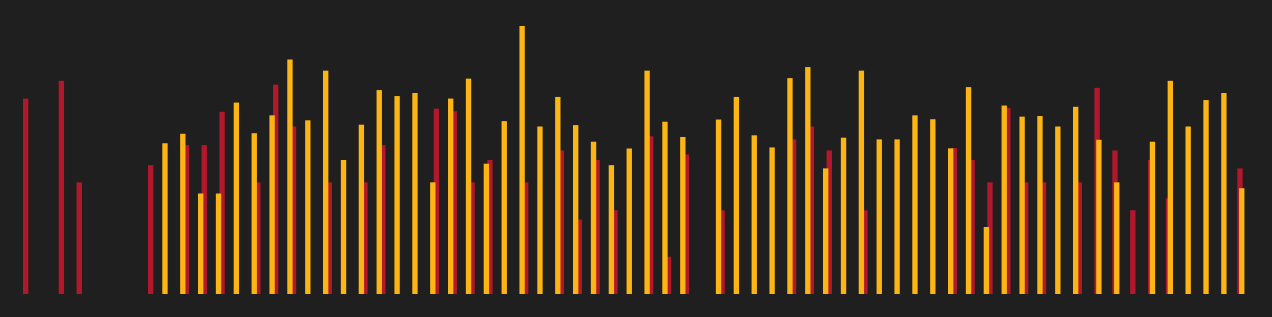
\includegraphics[scale=.25]{pics/bars_zvp.png}
  \caption{Protoss vs. Zerg win rates over time; Yellow is Protoss, Red is Zerg}
\end{figure}

\subsection{Finding High-Performing Players}
Finding high-performing players was a difficult task.  Initially, the approach of simply comparing player win rates was attempted, but was a miserable failure.  One critical feature of this datset was that there are a large number of distinct players, and most of them have only played a few matches (specifically, these are players that played in one or two tournaments, and stopped playing afterwards).  Thus, comparing win rates for players that have played 2-5 matches is clearly unfair to players who have played hundreds of matches.\\
In professional StarCraft, playing more matches is also indicative of skill.  In order to get invited to more tournaments, players must perform well in previous tournaments or risk being dropped from the professional scene altogether.  Therefore, one key observation was that the number of games played is a significant indicator for player skill.\\
Thus, we settled on using a standard rating for a binomial proportion, known as the lower bound of the Wilson score:
\[
\frac{{ {\hat p + \frac{{1}}{{2n}}
 z_{1- \alpha / 2}^2  \pm z_{1- \alpha / 2}
\sqrt {\frac{{\hat p\left( {1 - \hat p} \right)}}{n} + \frac{{z_{1- \alpha / 2}^2}}
{{4n^2}} }} }}
{{ {1 + \frac{{1}}{n}} z_{1- \alpha / 2}^2 }}
\]\\
This ended up as a very strong indicator for strong players - players regarded as the best StarCraft players also had a very high skill confidence.  We also found players who were not as highly regarded amongst the high ratings - one Protoss player was found to have many games played and a ~60\% win rate, and wasn't noticed by the public.  This was due to his relatively low exposure by the media, although he was performing at a top-tier level.

\subsection{Race Balance in the Professional Scene}
Another idea we wanted to visualize was racial balance in the professional scene.  Each race plays differently and one race may be vastly favored in a particular matchup.  In this visualization, we wanted to find if racial imbalances really existed in the professional Starcraft scene.  To do this, we took win percentages for each race, and compared them over time.\\

We can see that Protoss win rates are significantly higher than Zerg win rates for at least half the time period shown in the chart.  Until about 60\% of the way through, Protoss players have consistently had higher win rates than Zerg players.  However, after a little more than halfway through, Zerg win rates begin significantly increasing (and frequently outperforming Protoss win rates).  This point is actually in mid-September 2011, when a balance patch was released for StarCraft increasing the effectiveness of Zerg units.  This shifted the professional metagame for awhile, reducing Protoss win rates significantly.


\section{Data Transformation}
\subsection{Preprocessing and API}

In order to interface with the machine learning system, the data must be coerced to a specific format:

\begin{verbatim}
  player_entry = {
    'data': numpy.array([[feature1, feature2, ...],
                          ...
                        ]),
    'outcomes': numpy.array([outcome1, outcome2, ...])
  }
\end{verbatim}

where each element of the \verb$data$ array represents features of a match resulting in the correspondingly indexed \verb$outcome$.

To build the features, we load the CSV files from the scraper script through Pandas, after which time we can gather various statistics, such as win percentage for a given player against another player, race, or map, that will be used as features in the prediction models later on. 

This processing script exposes two API calls: \verb$process_data()$ and \verb$get_feature(input)$. The former is run once per data scrape, and generates the above \verb$player_entry$ records for every player in the dataset for use in training models in the next stage. The latter returns a player's feature vector for online predictions, given situational input variables including prediction date, map id, and both players' ids.

\subsection{Persistence}

There is also another non-API function in the preprocessing script for persisting the data; while regenerating all features from the CSV is most accurate, it also performs too slowly for online predictions (on the order of 1 minute per prediction on an EC2 micro instance). To alleviate this we cache intermediate calculations in a MongoDB database, allowing our program to recall and/or recalculate features in real-time.

\section{Data Product}
From all these Starcraft 2 match results, one possible data product that crossed our mind was a predictor that could predict the victor of a match given the players involved and the map they are playing. With this goal in mind, we proceeded as follows. 

\subsection{Models}
To tackle this problem, we approached it as a classification problem. More specifically, we could train a classifier model on a player's past matches, then feed it upcoming match data. The output would simply be a binary classification (i.e. \textbf{lose} or \textbf{win}). Through the miracles of scikit-learn, we were able to experiment with the following models:

\begin{enumerate}
\item Logistic Regression
\item Decision Trees
\item Multinomial Bayes
\item Support Vector Machine
\item Random Forests
\item Stacking Ensembles
\begin{enumerate}
\item Logistic Regression
\item Multi-Response Linear Models
\end{enumerate}
\end{enumerate}

For more information on these models, it is sufficient to either Google or Wikipedia for the terms.

\subsection{Features}
Before tinkering with the models, we put a bit of thought on what features would characterize a player's performance. Though there are some established metrics, particularly the infamous APM, we discounted this on the basis that on the professional stage, the level of game mechanics is on an equal level among the players. Instead, the decisions that a player makes against his or her opponent is the biggest factor on victory. At this high level, the strategies one chooses is dependent on two things: the opponent's race and the map being played. Keeping this in mind, we began with the following features:

\begin{enumerate}
\item \textbf{player's win rate against opponent's race on map} - For a professional player, they tend to usually select a specific strategic based on which map they are on and what race they are playing against. This metric seems to capture the player's accuracy in selecting a successful strategy.
\item \textbf{opponent's win rate against player's race on map} - For the same reasons above, we included this for the opponent.
\item \textbf{player's win rate against opponent overall} - Considering how players tend to study their opponents tactics, this metric seems to capture how accurately a player can read their opponent.
\item \textbf{time} - It made sense to factor in time to account for Starcraft 2's constantly changing metagame due to patches and evolving plays.
\end{enumerate}

The results for these features can be seen in \ref{sec:evaluation1}. With some thought, we stumbled on these additional features:

\begin{enumerate}
\setcounter{enumi}{4}
\item \textbf{player's win rate on map} - After some consideration, it hit upon us that players also tend to take advantage of some features of a map on the fly during a match, which is potentially modeled in this feature.
\item \textbf{opponent's win rate on map} - For the same reasons above, we included this for the opponent.
\item \textbf{player's win rate against opponent's race} - With further thinking, we also realized that players are not limited to using specific strategies for a race based on a map. To factor this in, we felt that this feature was the closest indicator of the success of a player's strategy.
\item \textbf{opponent's win rate against player's race} - For the same reasons above, we included this for the opponent.
\end{enumerate}

The results for these features can be seen in \ref{sec:evaluation2}. Yet, with some more thoughts, we figured out one additional feature:

\begin{enumerate}
\setcounter{enumi}{8}
\item \textbf{player's win rate against opponent on map} - Keeping in mind how players have an intuitive idea of what tricks their opponents may try on a specific map, this feature seemed to be the best choice for representing this intuition.
\end{enumerate}

\subsection{Evaluation of Models}
\label{sec:evaluation}
As noted in the above sections, we evaluated each model we had on multiple feature sets. To do these evaluations, we ran a 10-fold cross validation on each model with the given features, plotted ROC curves for each fold, then examined the average ROC curve. For the actual player, we settled on using MVP, a well known Terran player with an average amount of matches.

\subsubsection{Features 1-4}
\label{sec:evaluation1}
Refer to Figure \ref{fig:fig1} for the results. From a quick inspection at the overall AUC average, the feature selection seems to be pretty good. However, considering the variance in the ROC curves for a majority of the models, it seems as if any of these models will not have consistent performance. From comparing the models, it's clear that the stacking MLR model is the best.

\subsubsection{Features 1-8}
\label{sec:evaluation2}
Refer to Figure \ref{fig:fig2} for the results. Compared to the results in \ref{sec:evaluation1}, the changes are very minimal, which seems to imply that a few of the included features are redundant. In addition, these results indicate stacking MLR is once again the best choice.

\subsubsection{Features 1-9}
\label{sec:evaluation3}
Refer to Figure \ref{fig:fig3} for the results. Interestingly, including the player's win rate heavily improves the performance of all the models. However, as we point out in \ref{sec:selection}, this is actually an issue of leaking, or overfitting the data set. Yet, even though all the models are performing at a similar level, the stacking MLR is still the best choice overall.

\subsection{Selection of Models and Features}
\label{sec:selection}

From looking at the evaluations in \ref{sec:evaluation}, the most obvious choice in features would be using all the features. However, this is actually the worst one to use because any of the models overfits. Why is this the case? In a roundabout way, our models are actually trying to predict the win rate of the player against the opponent on that specific map. Clearly, if we give the model this value as a feature, it's simply going to fit only on that as a feature. As a result, it overfits and yields lopsided values. With this in mind, it was clear that the best choice would then be features used in \ref{sec:evaluation2}, as these were the next best without overfitting. Finally, since stacking MLR was consistently the best performer, we chose this as our model.

\subsection{Model Predictions}
To test drive our model, we decided to predict the outcome of recent matches played in the GSL Code S League. The results are as follows:

NOTE: Percentages indicate player's chance of winning according to the model. Ties in classification are broken by which model's confidence is higher.

\begin{center}
\begin{tabular}{| l | l | l | l | l | l | l | l |}
\hline
Map & P1 & P2 & P1's \% & P2's \% & Prediction & Actual \\
\hline
Cloud Kingdom & Parting & TheStC & 93\% & 3\% & Parting & Parting \\
Antiga Shipyard & Parting & TheStC & 82\% & 1\% & Parting & Parting \\
Atlantis Spaceship & MarineKing & TaeJa & 12\% & 83\% & TaeJa & MarineKing \\
Cloud Kingdom & MarineKing & TaeJa & 3\% & 95\% & TaeJa & MarineKing \\
Metropolis & Parting & MarineKing & 35\% & 95\% & MarineKing & Parting \\
Entombed Valley & Parting & MarineKing & 1\% & 98\% & MarineKing & MarineKing \\
Daybreak & Parting & MarineKing & 25\% & 25\% & MarineKing & Parting \\
Metropolis & TheStC & TaeJa & 94\% & 1\% & TheStC & TaeJa \\
Daybreak & TheStC & TaeJa & 94\% & 5\% & TheStC & TaeJa \\
Entombed Valley & TaeJa & MarineKing & 13\% & 40\% & MarineKing & TaeJa \\
Dual Sight & TaeJa & MarineKing & 31\% & 14\% & TaeJa & TaeJa \\
\hline
\end{tabular}
\end{center}

From the above, there is something our model is lacking since it is only capable of predicting 4 out of 11 matches correctly - or in other words, it does worse then random guessing. It's clear that this is a good example of how simple validation is not always enough to guarantee actual success on new data.

\begin{figure}[t]
\centering
\subfloat[Logistic Regression]{
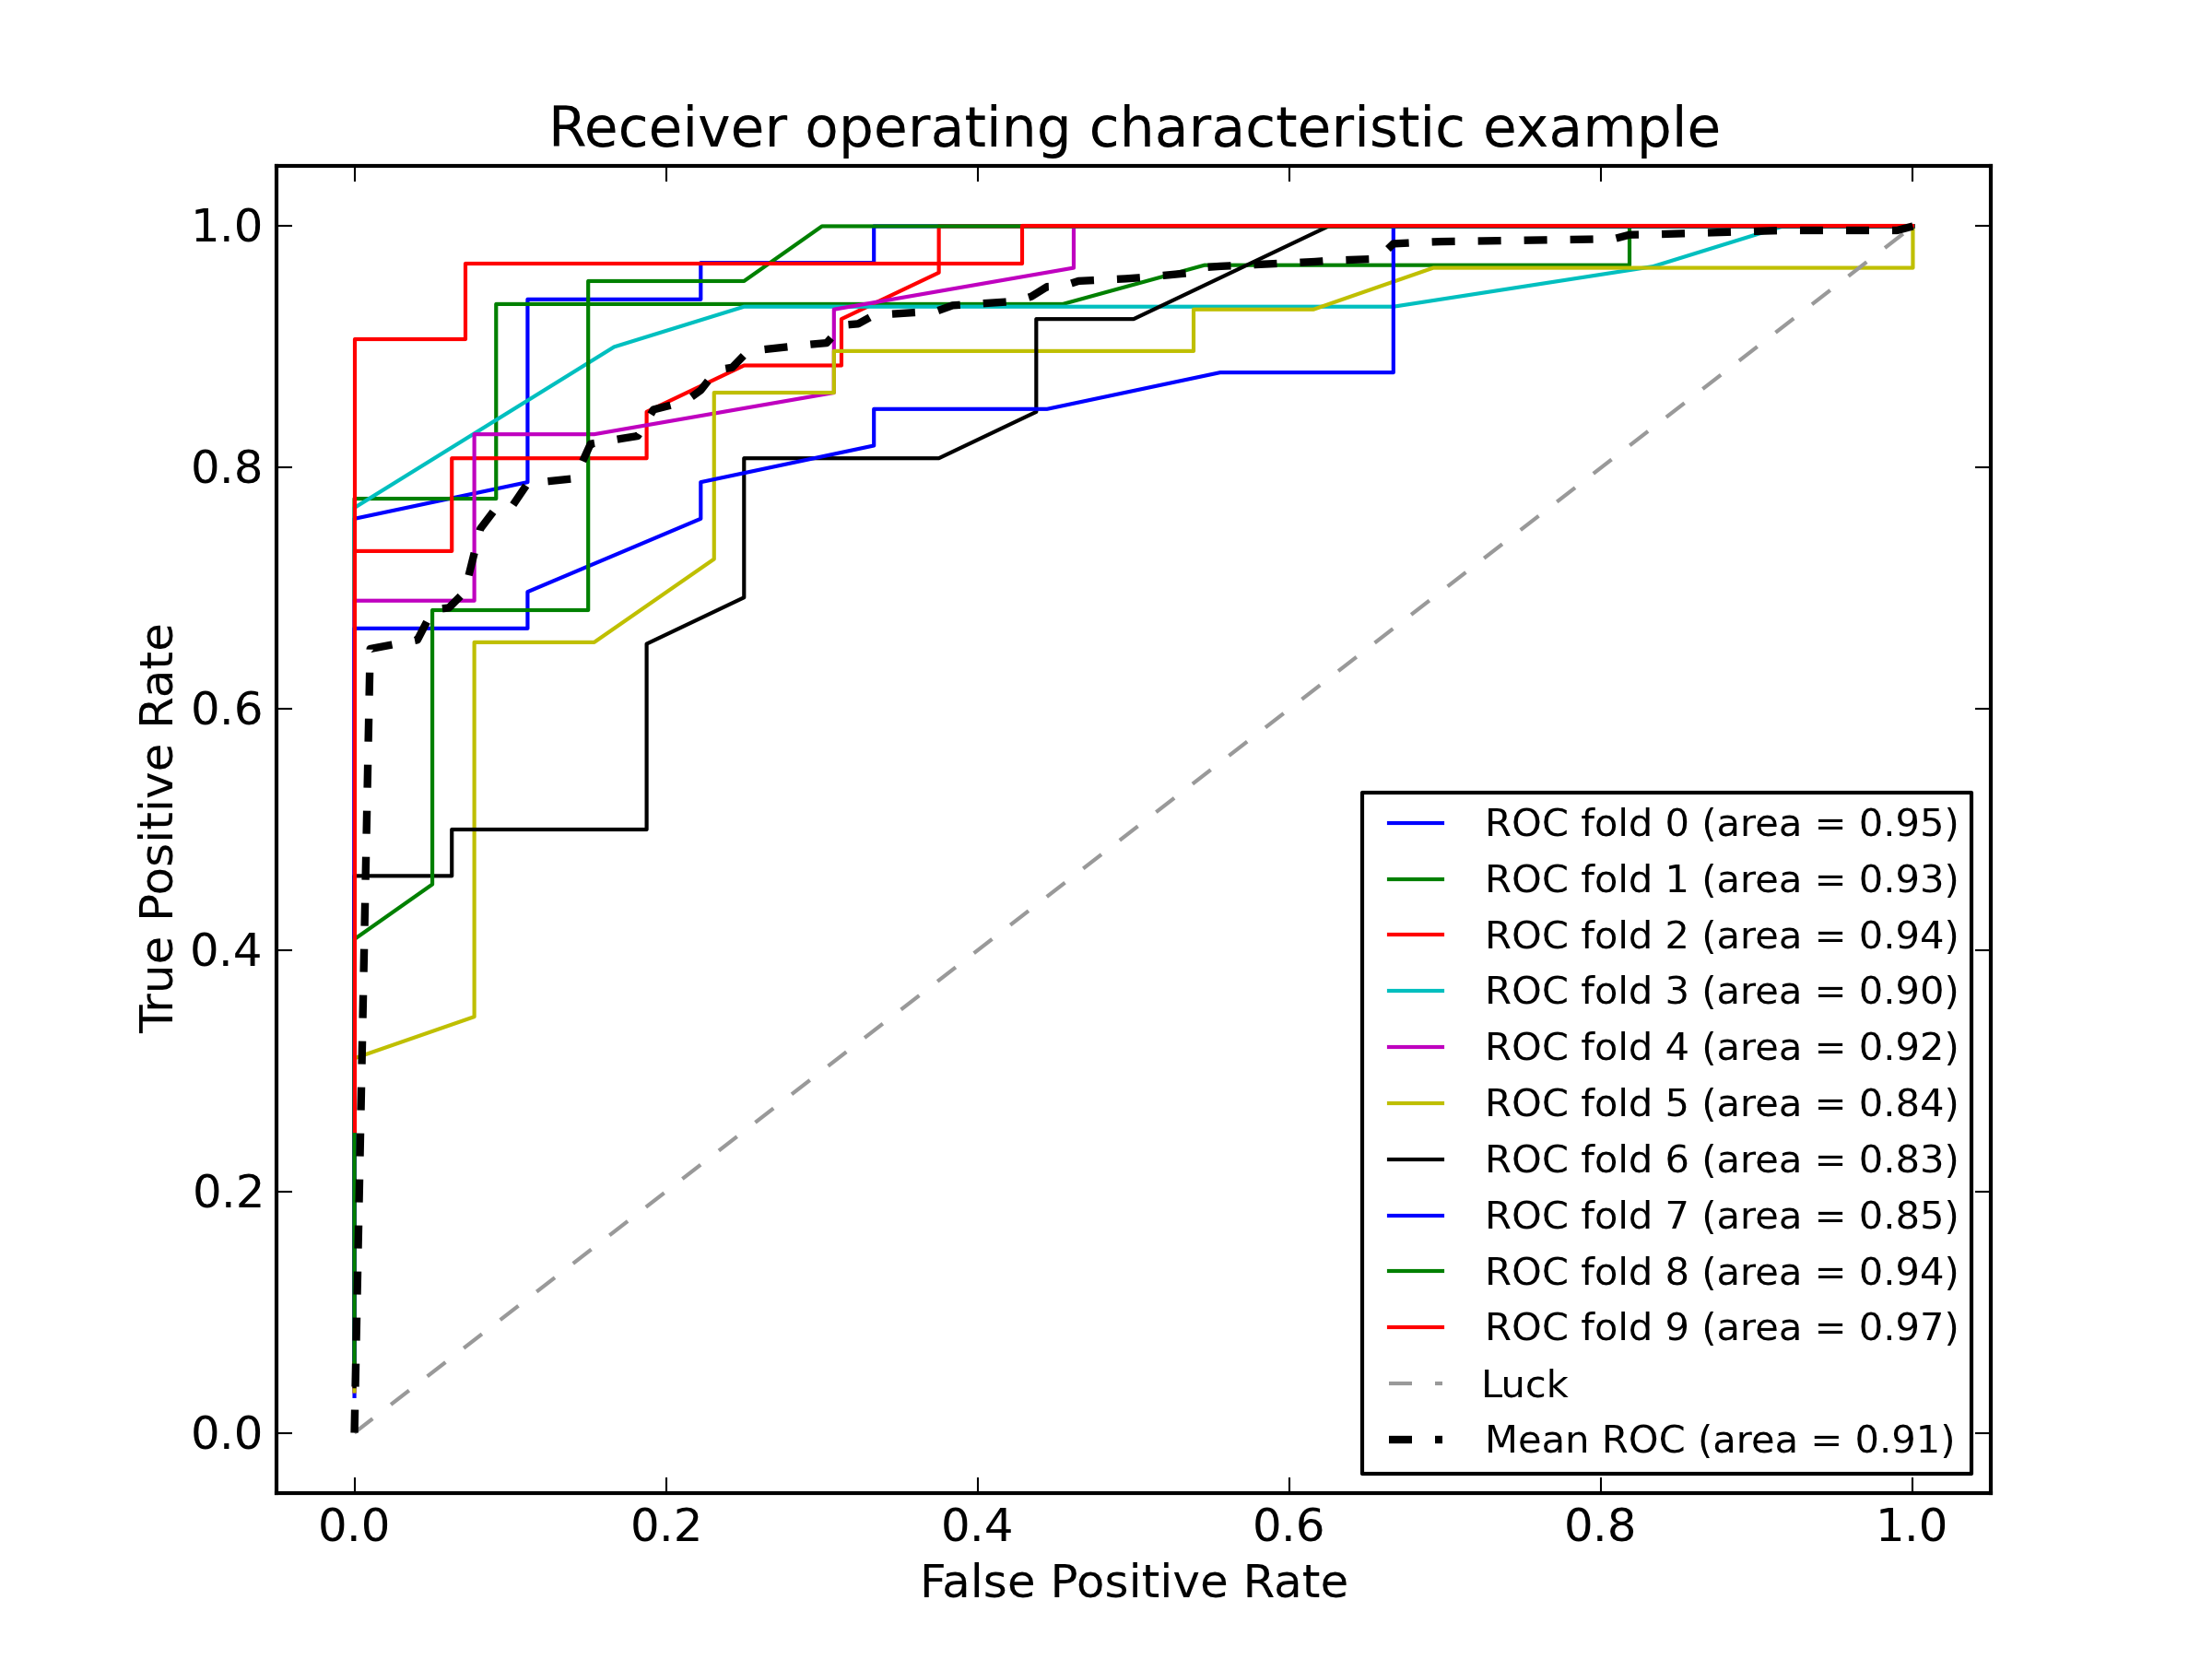
\includegraphics[width=0.36\textwidth]{pics/0_590_logit.png}}
\quad
\subfloat[Decision Trees]{
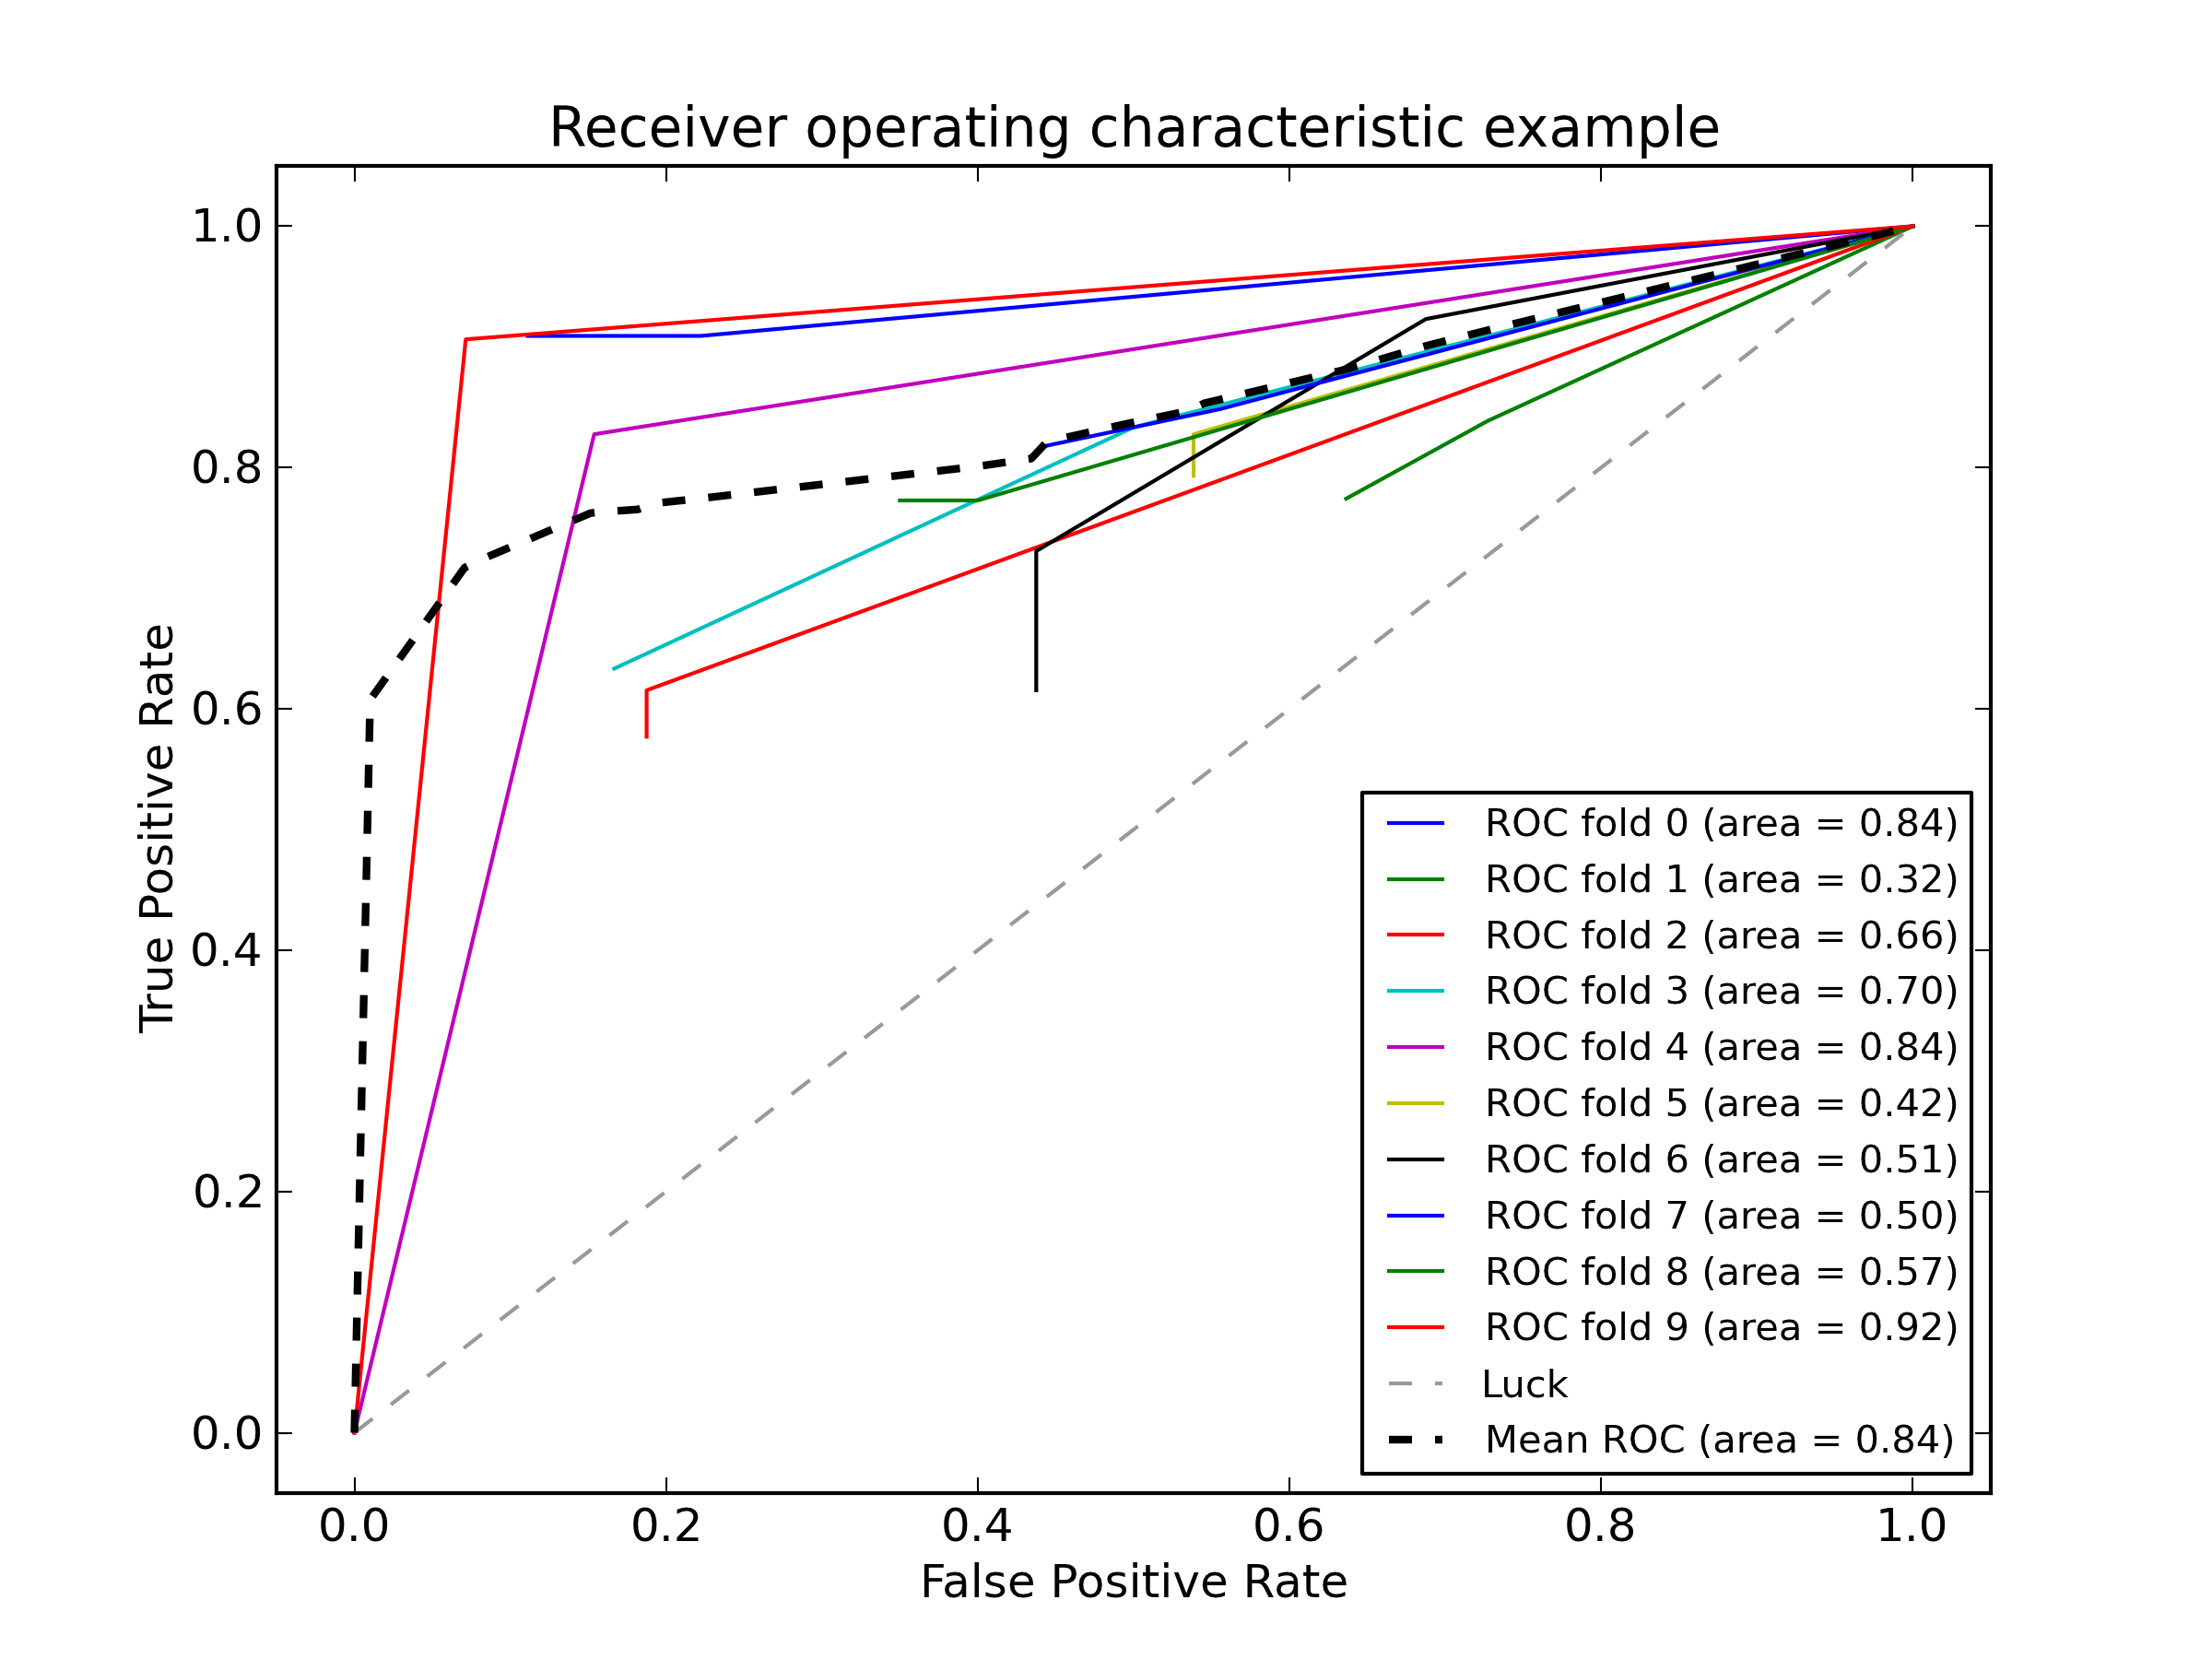
\includegraphics[width=0.36\textwidth]{pics/0_590_dtree.png}}
\quad
\subfloat[Multinomial Bayes]{
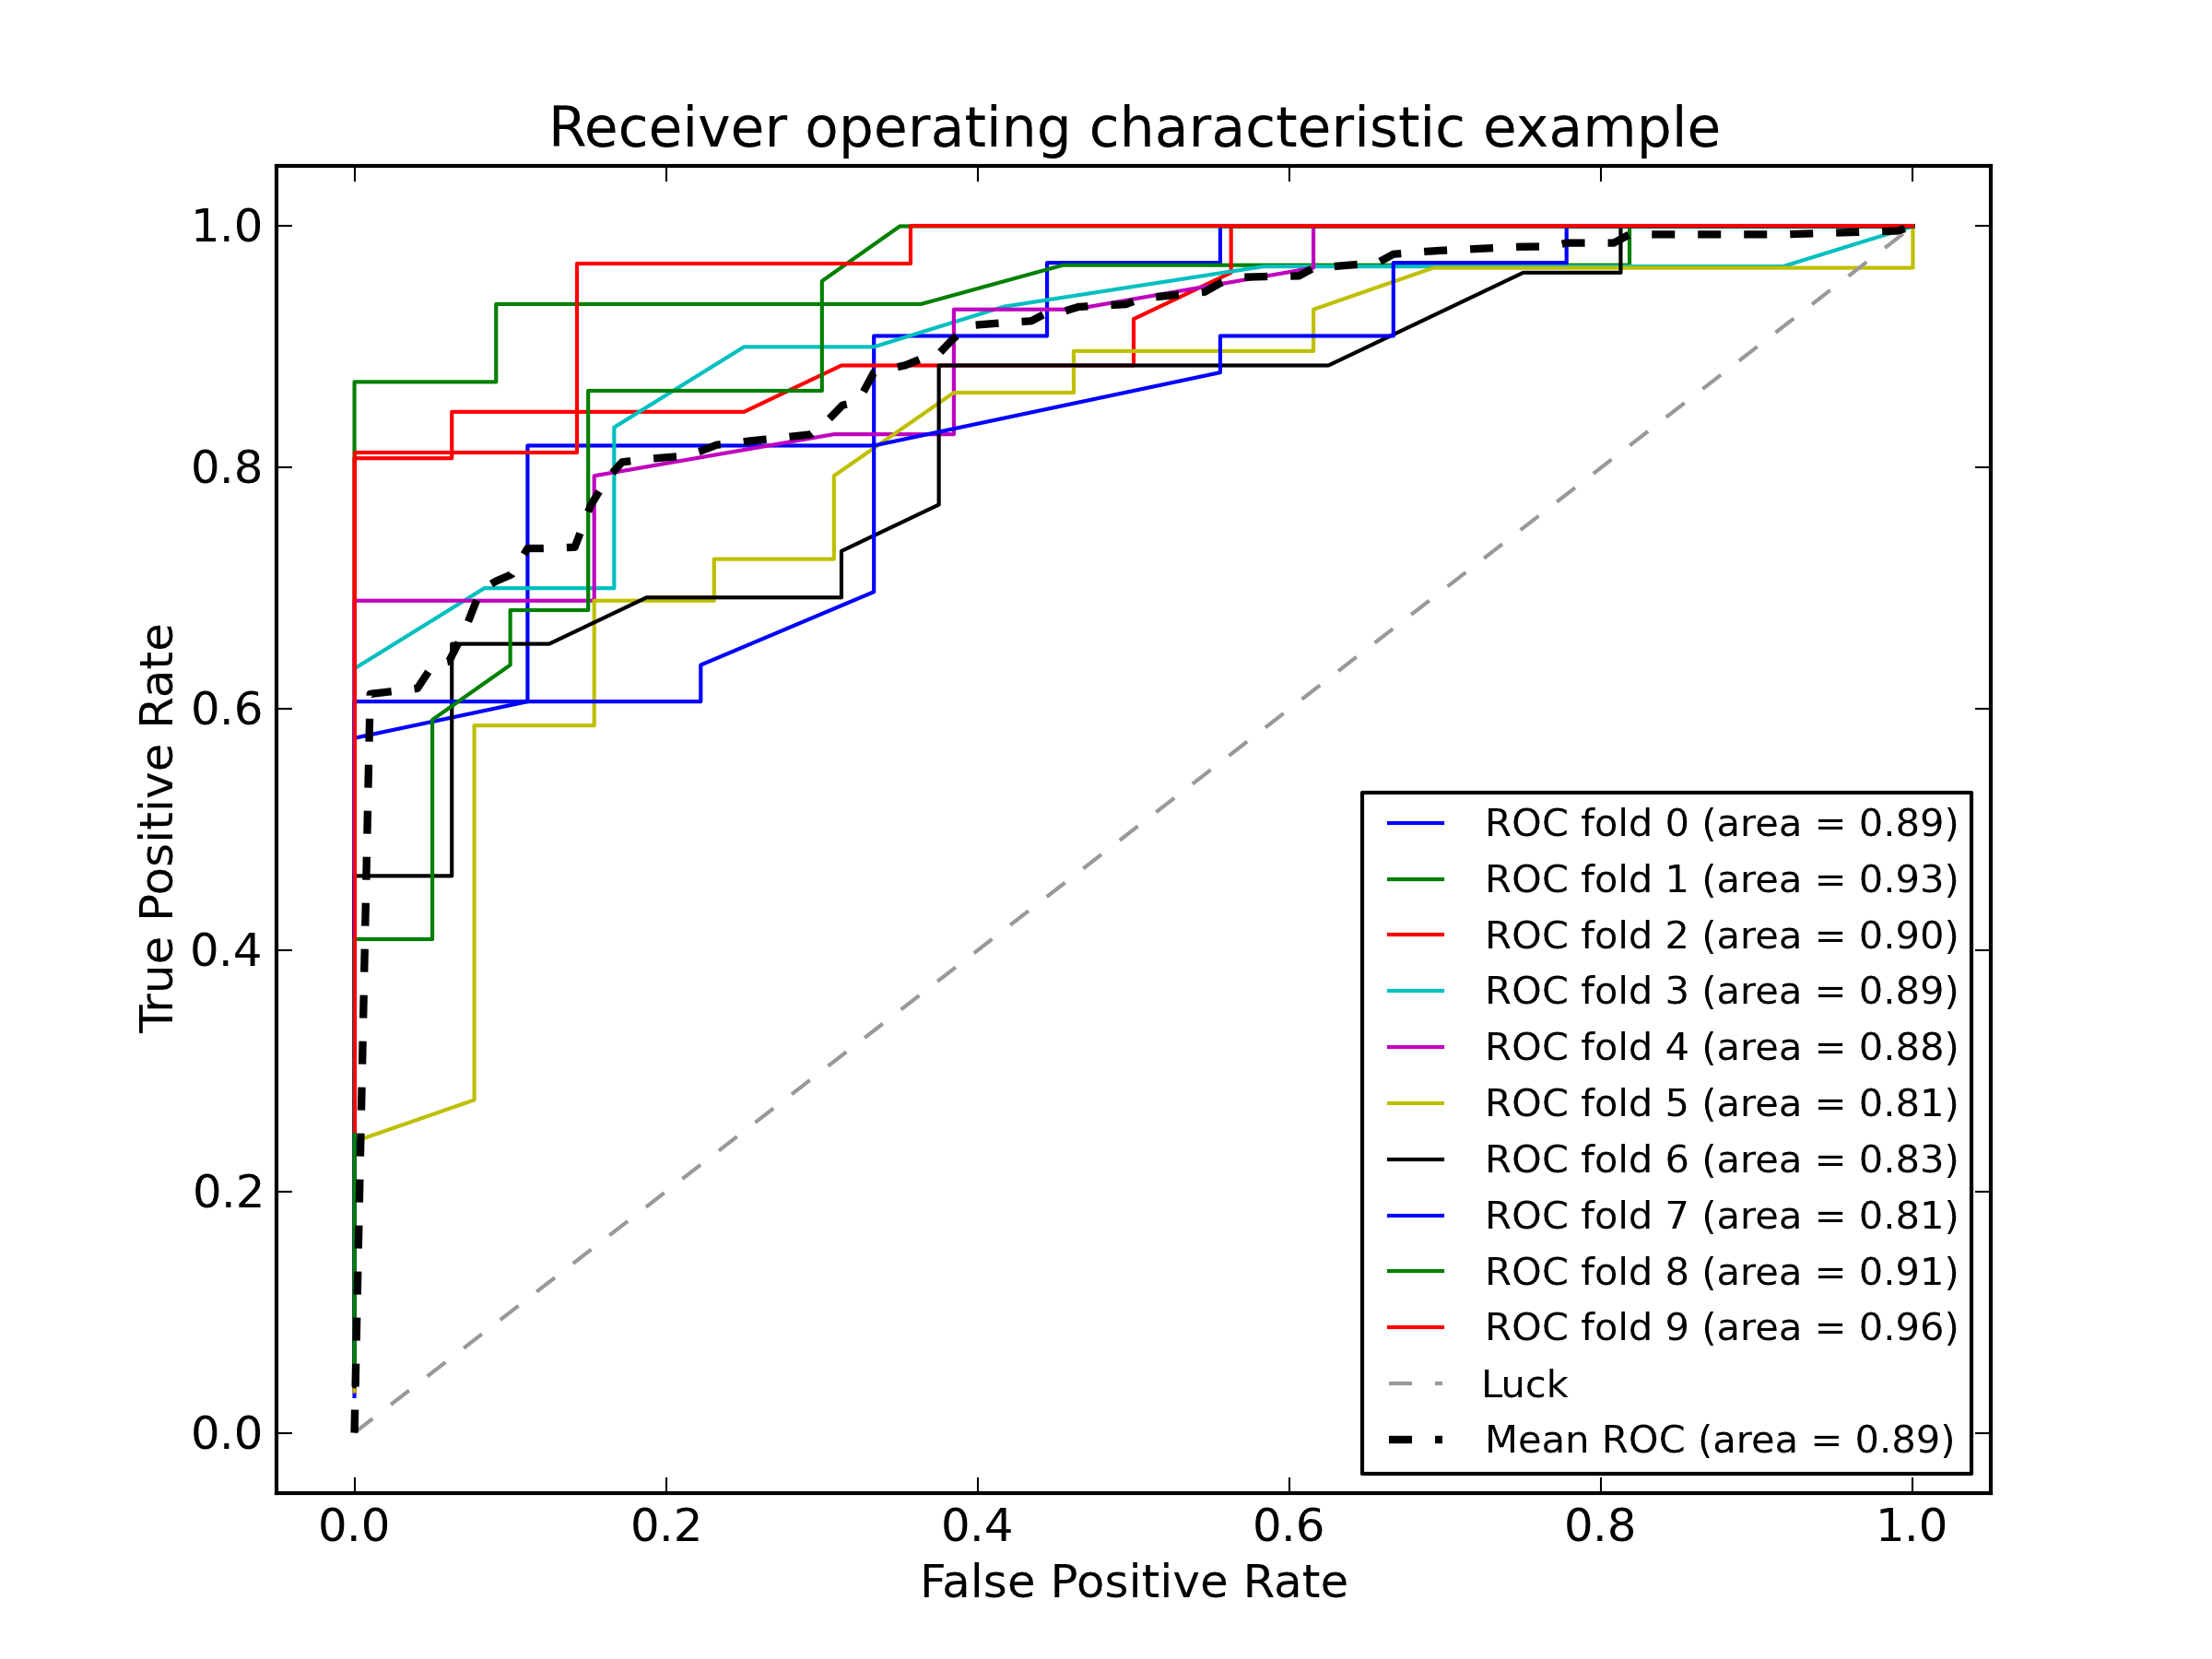
\includegraphics[width=0.36\textwidth]{pics/0_590_multi.png}}
\quad
\subfloat[Support Vector Machines]{
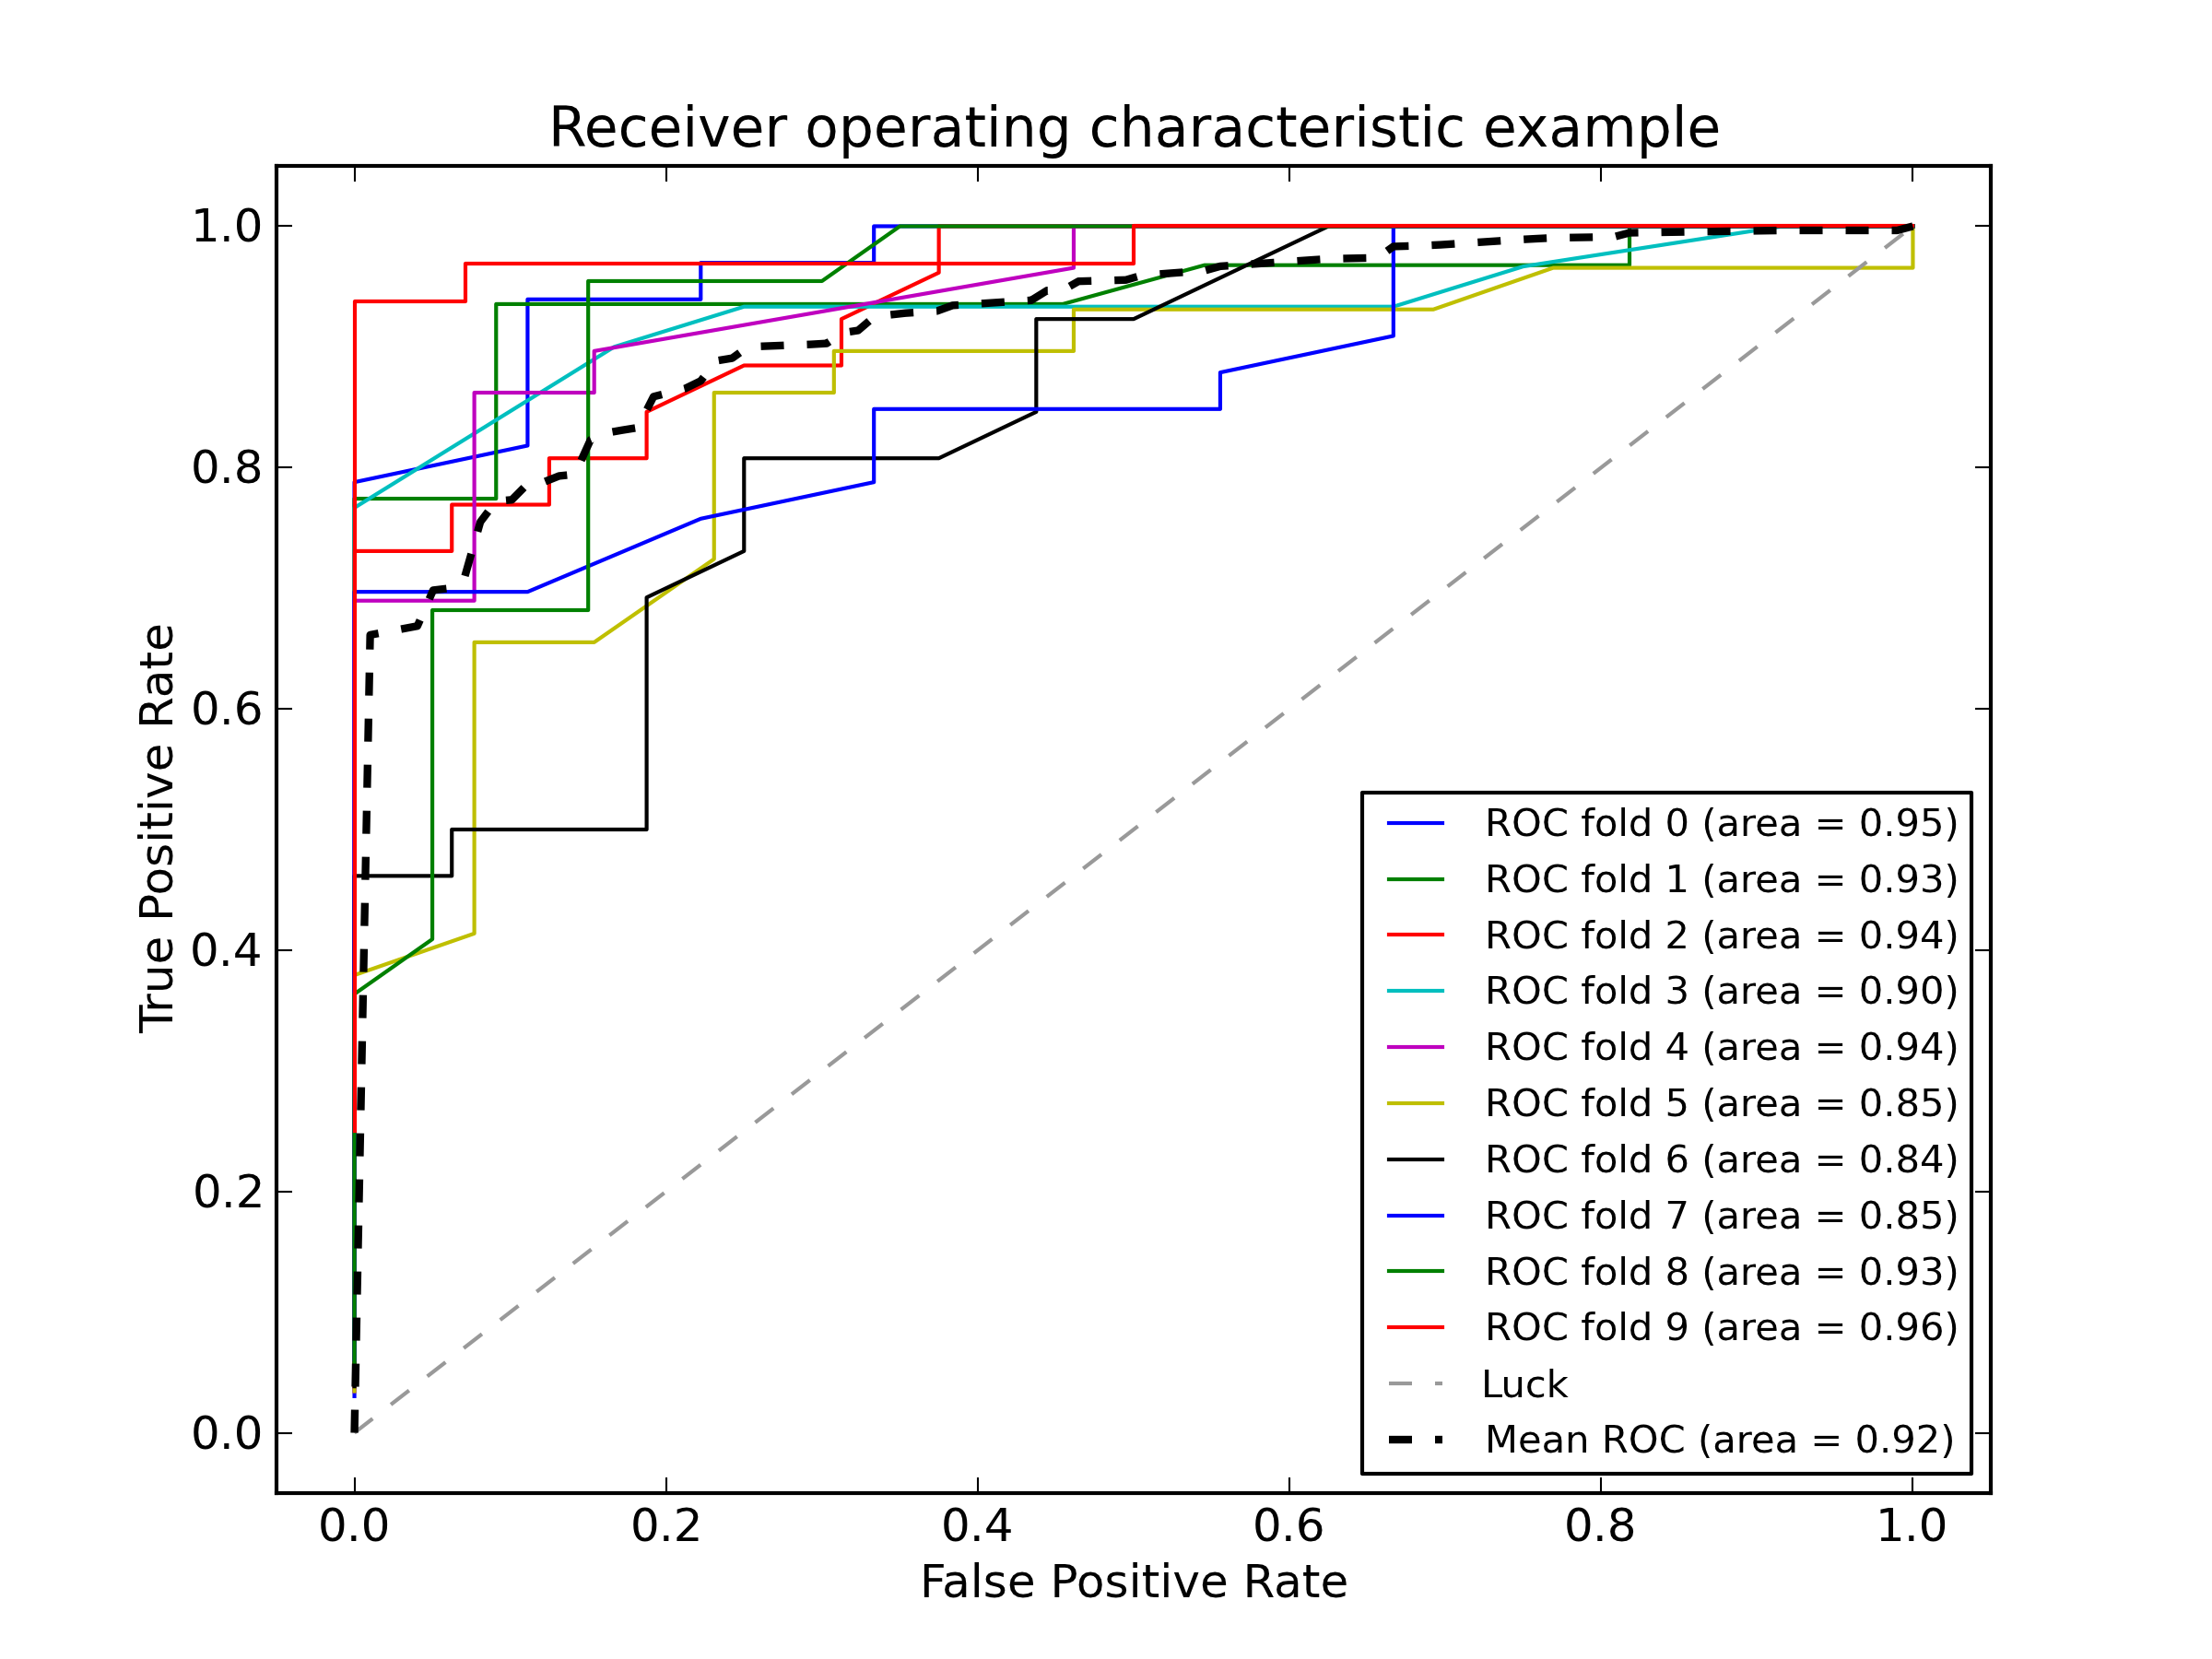
\includegraphics[width=0.36\textwidth]{pics/0_590_svm.png}}
\quad
\subfloat[Random Forests]{
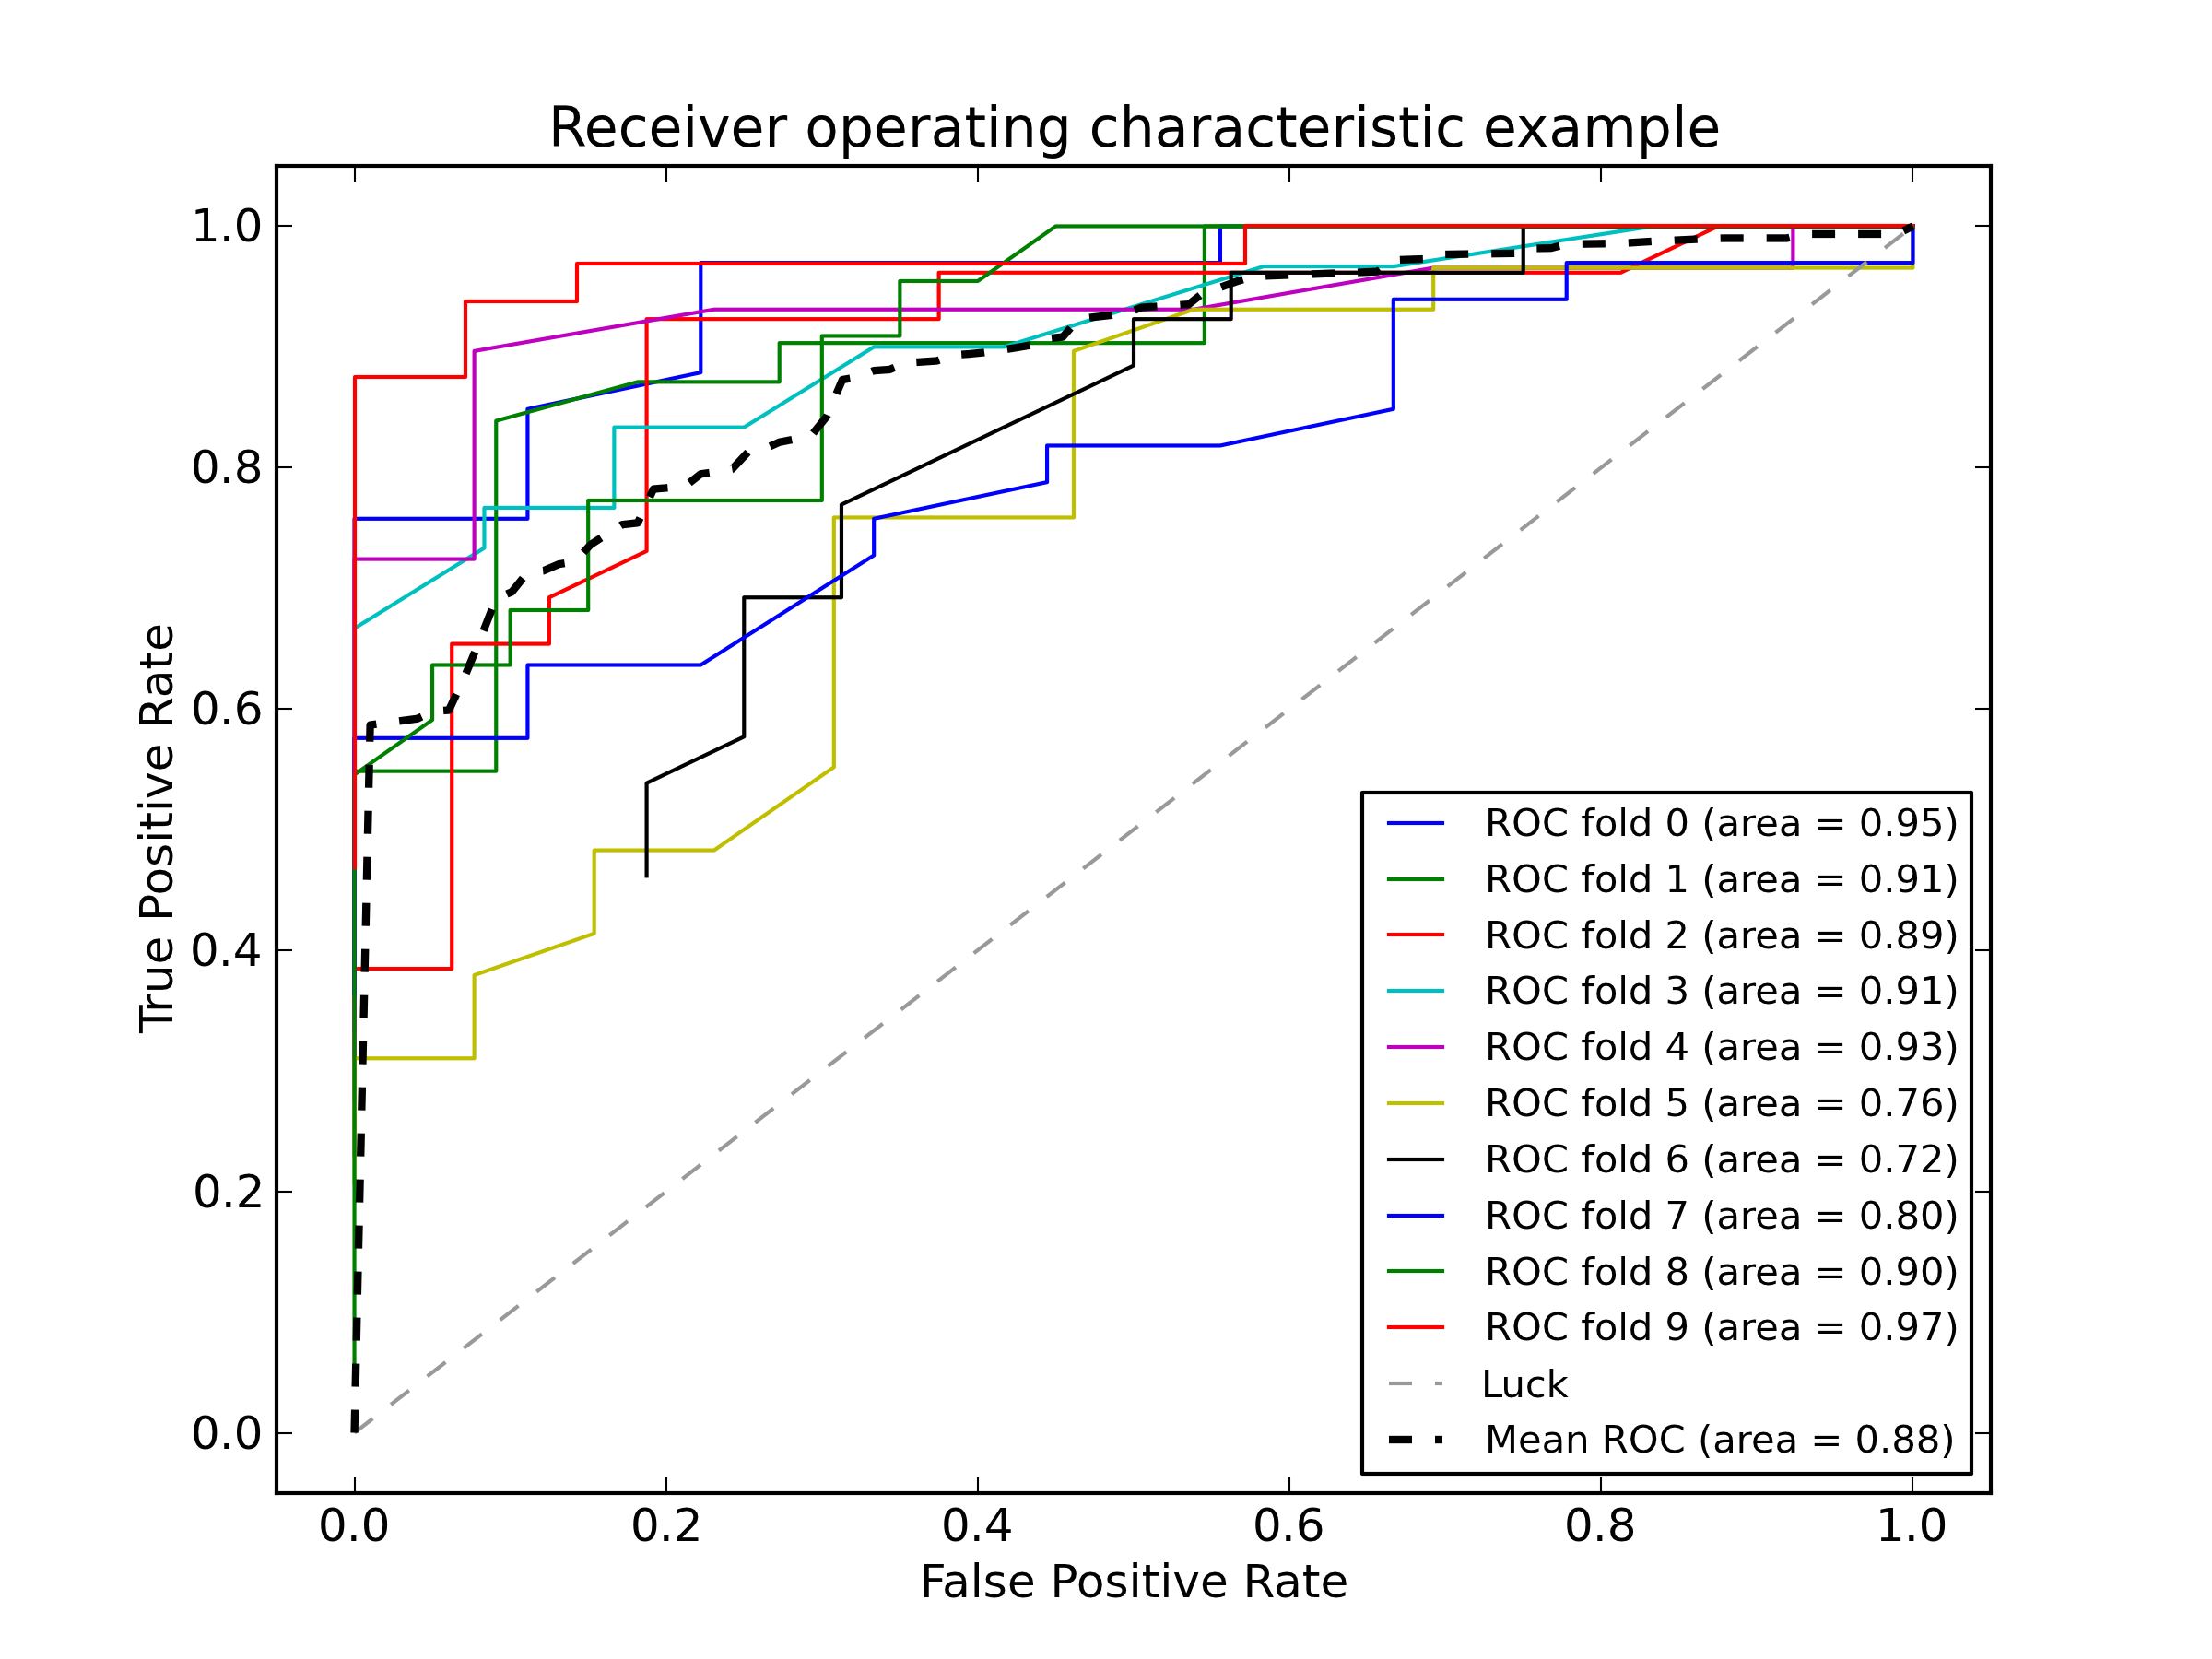
\includegraphics[width=0.36\textwidth]{pics/0_590_forest.png}}
\quad
\subfloat[Stacking - Logistic Regression]{
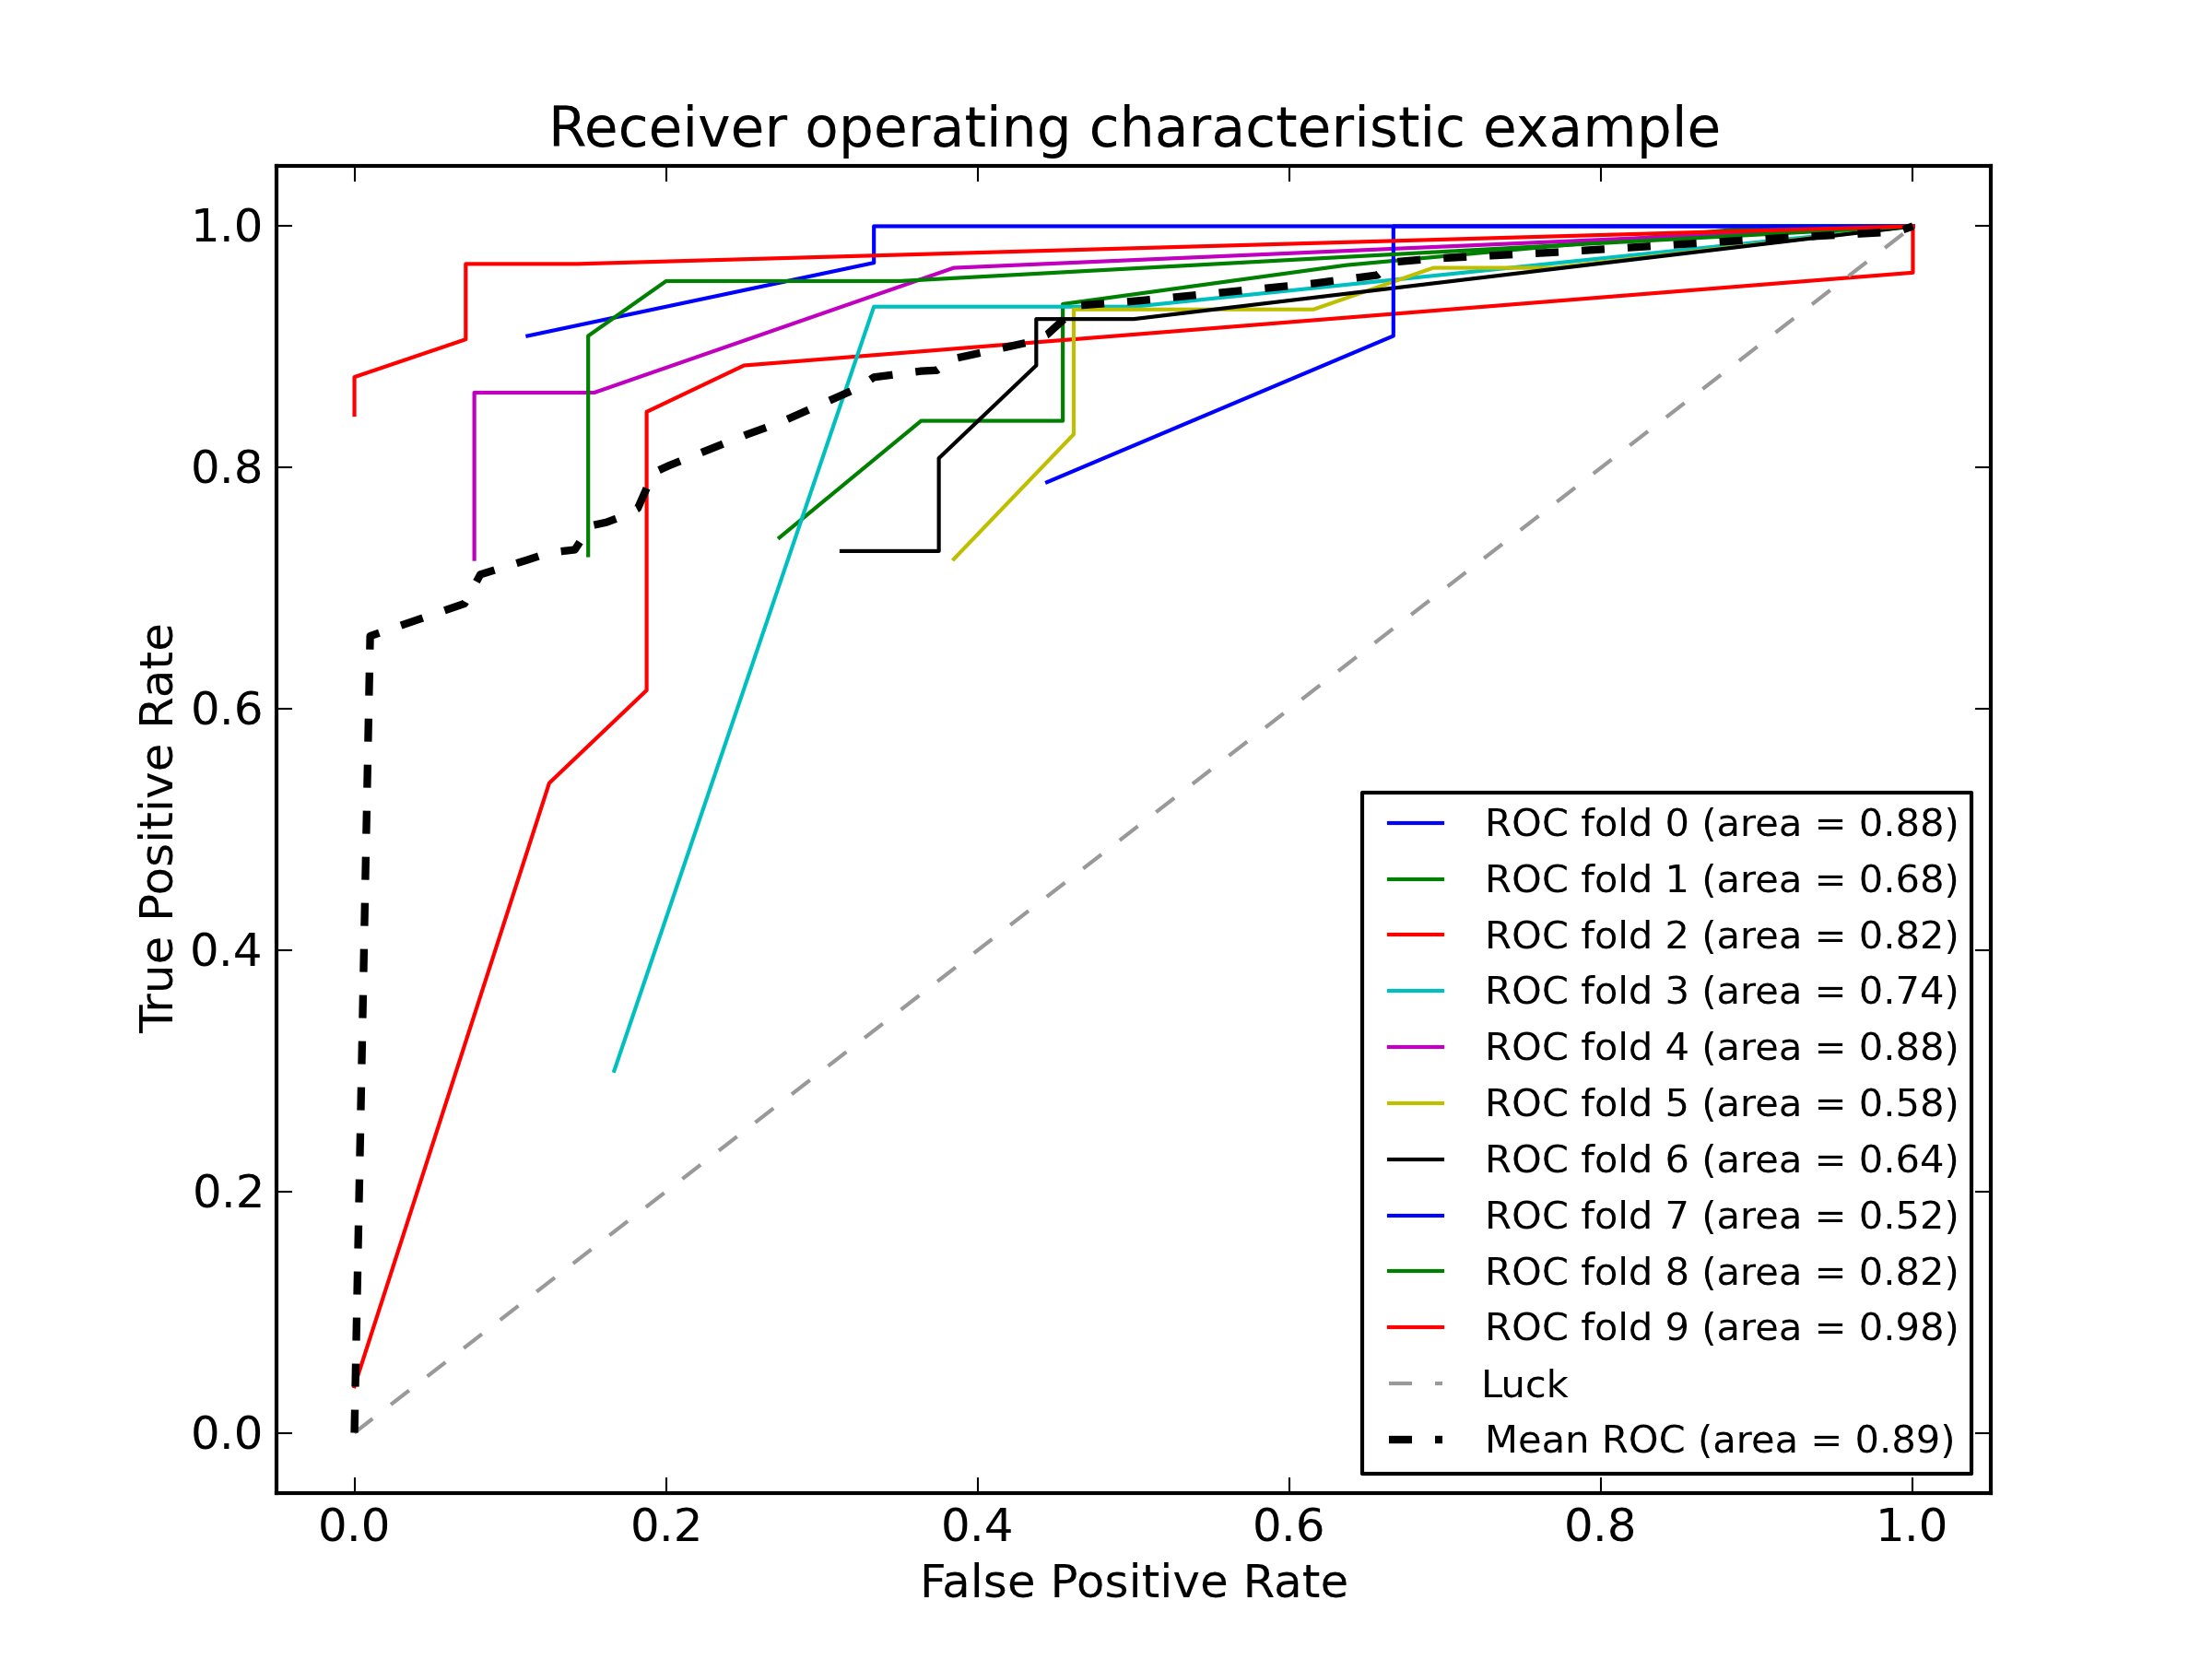
\includegraphics[width=0.36\textwidth]{pics/0_590_wmm.png}}
\quad
\subfloat[Stacking - Multi-Response Linear Models]{
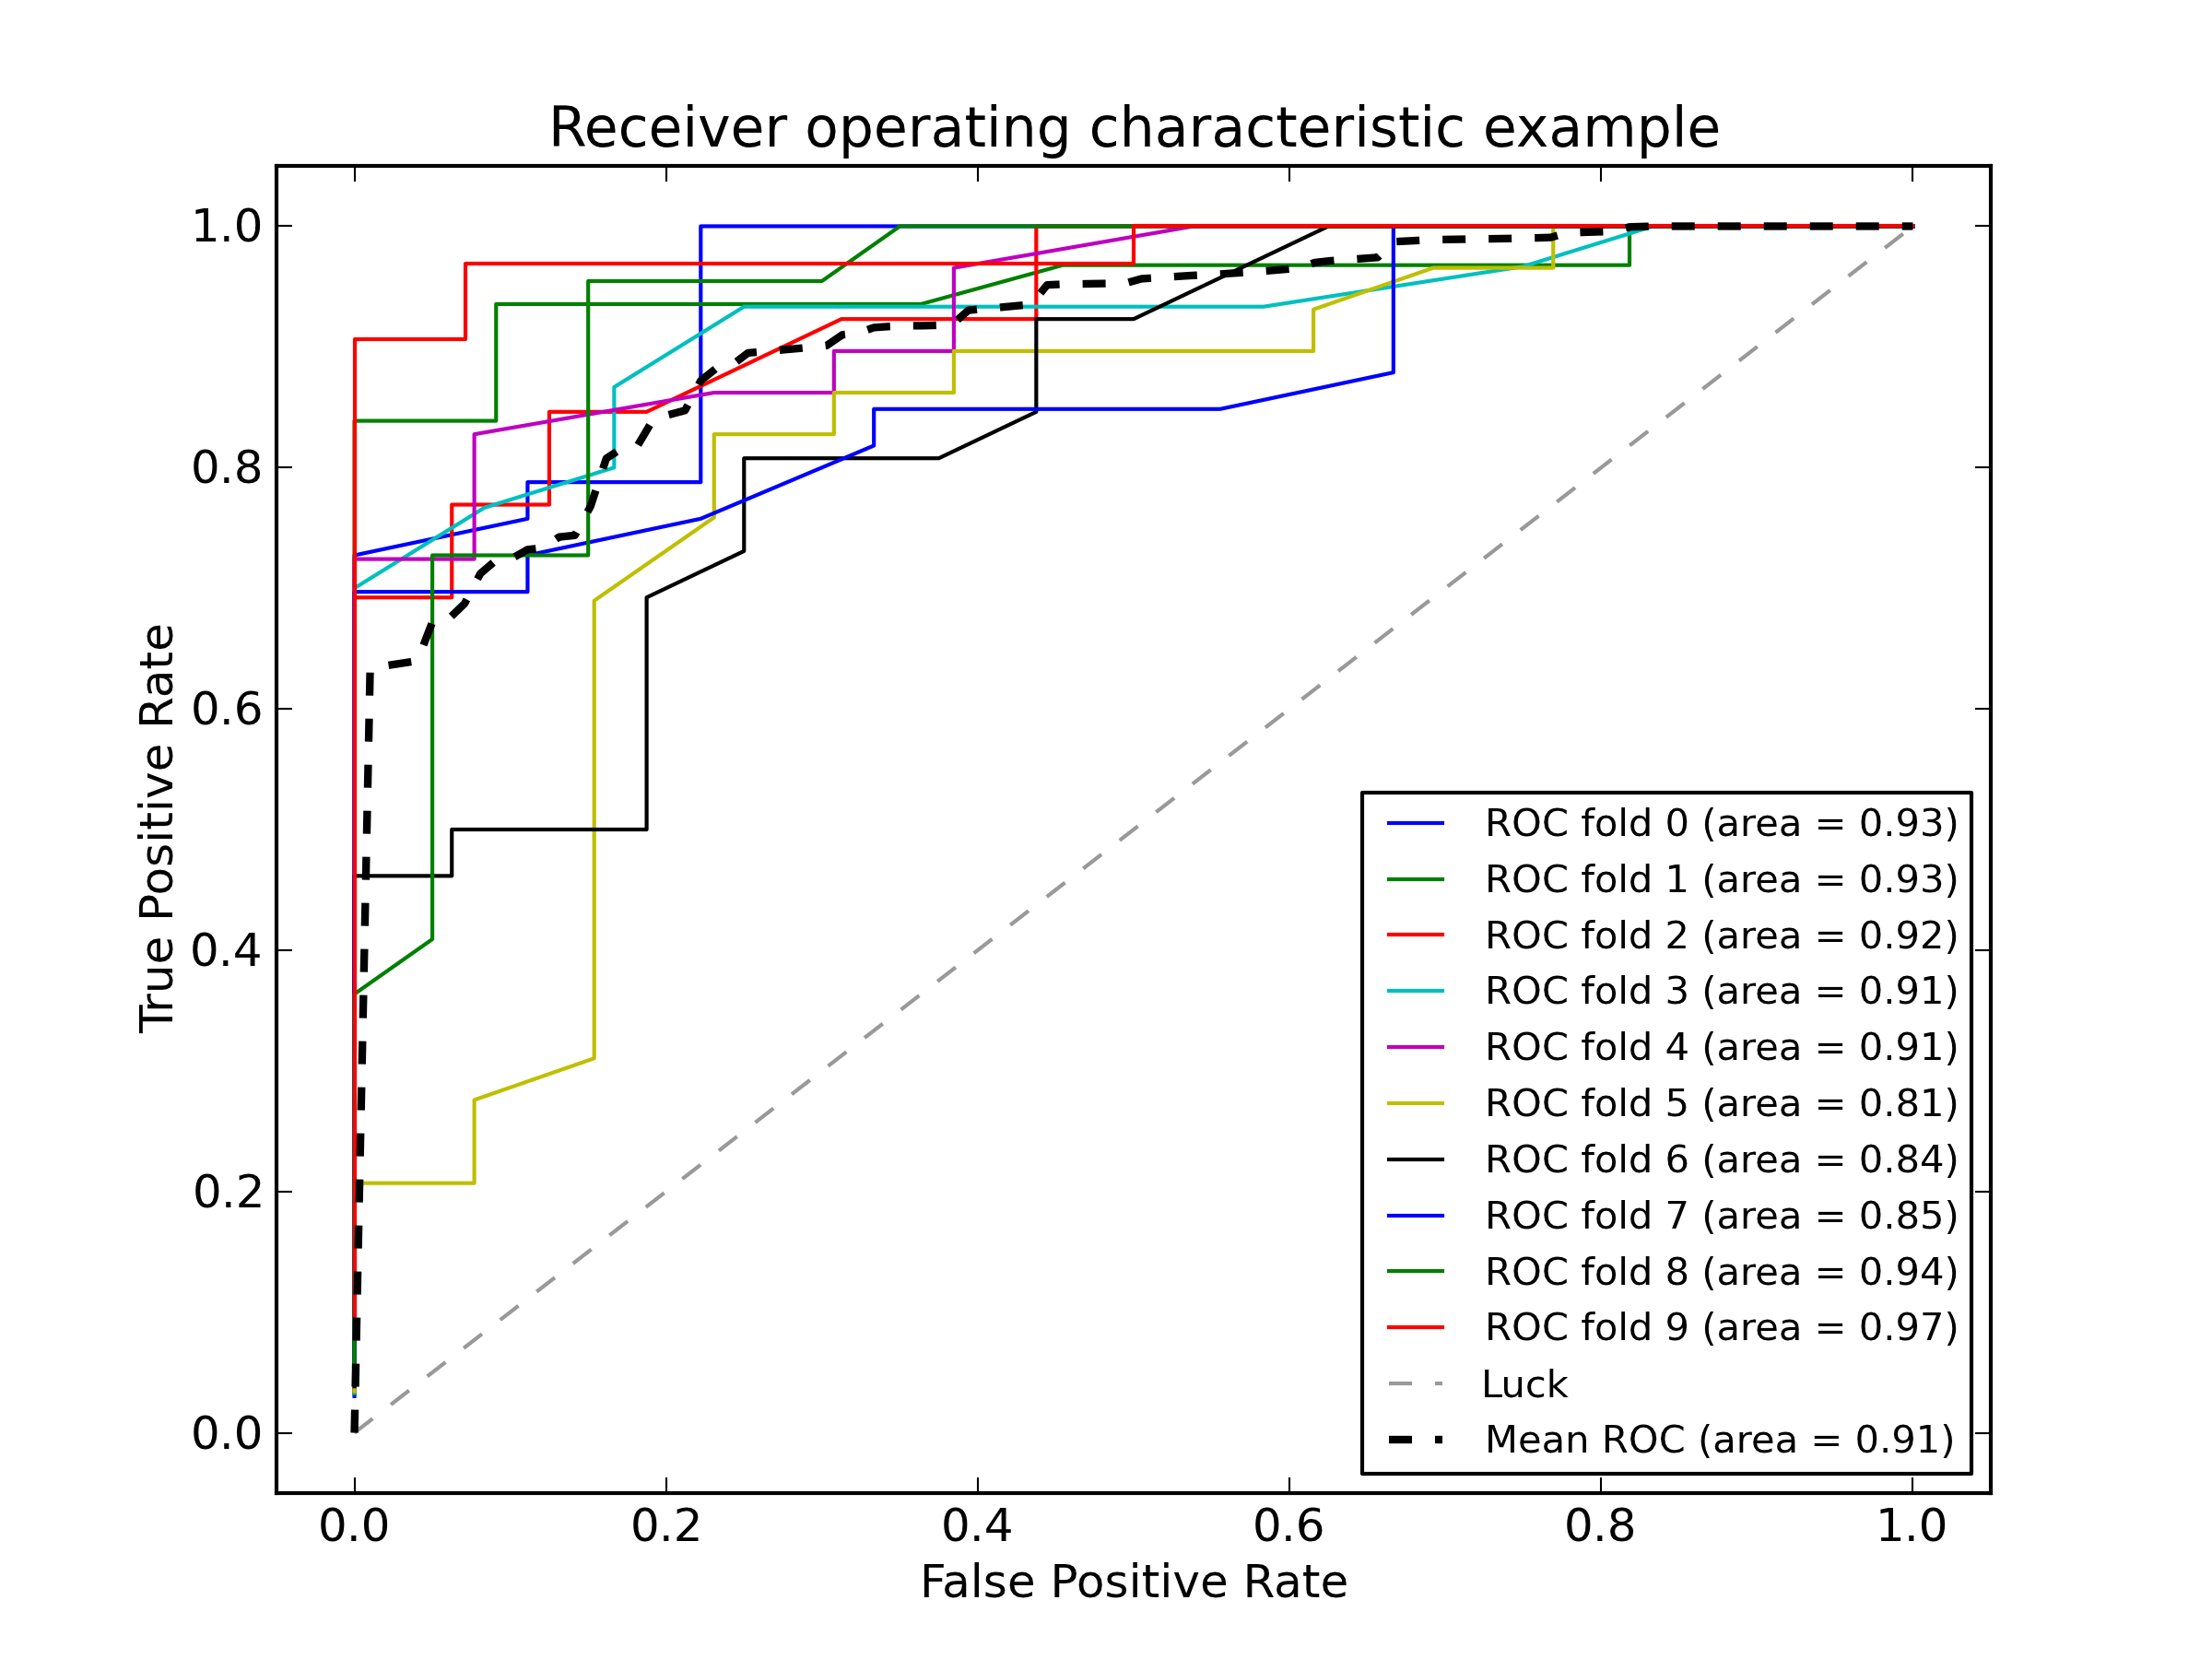
\includegraphics[width=0.36\textwidth]{pics/0_590_smm.png}}
\caption{Results for Features 1-4}
\label{fig:fig1}
\end{figure}

\begin{figure}[t]
\centering
\subfloat[Logistic Regression]{
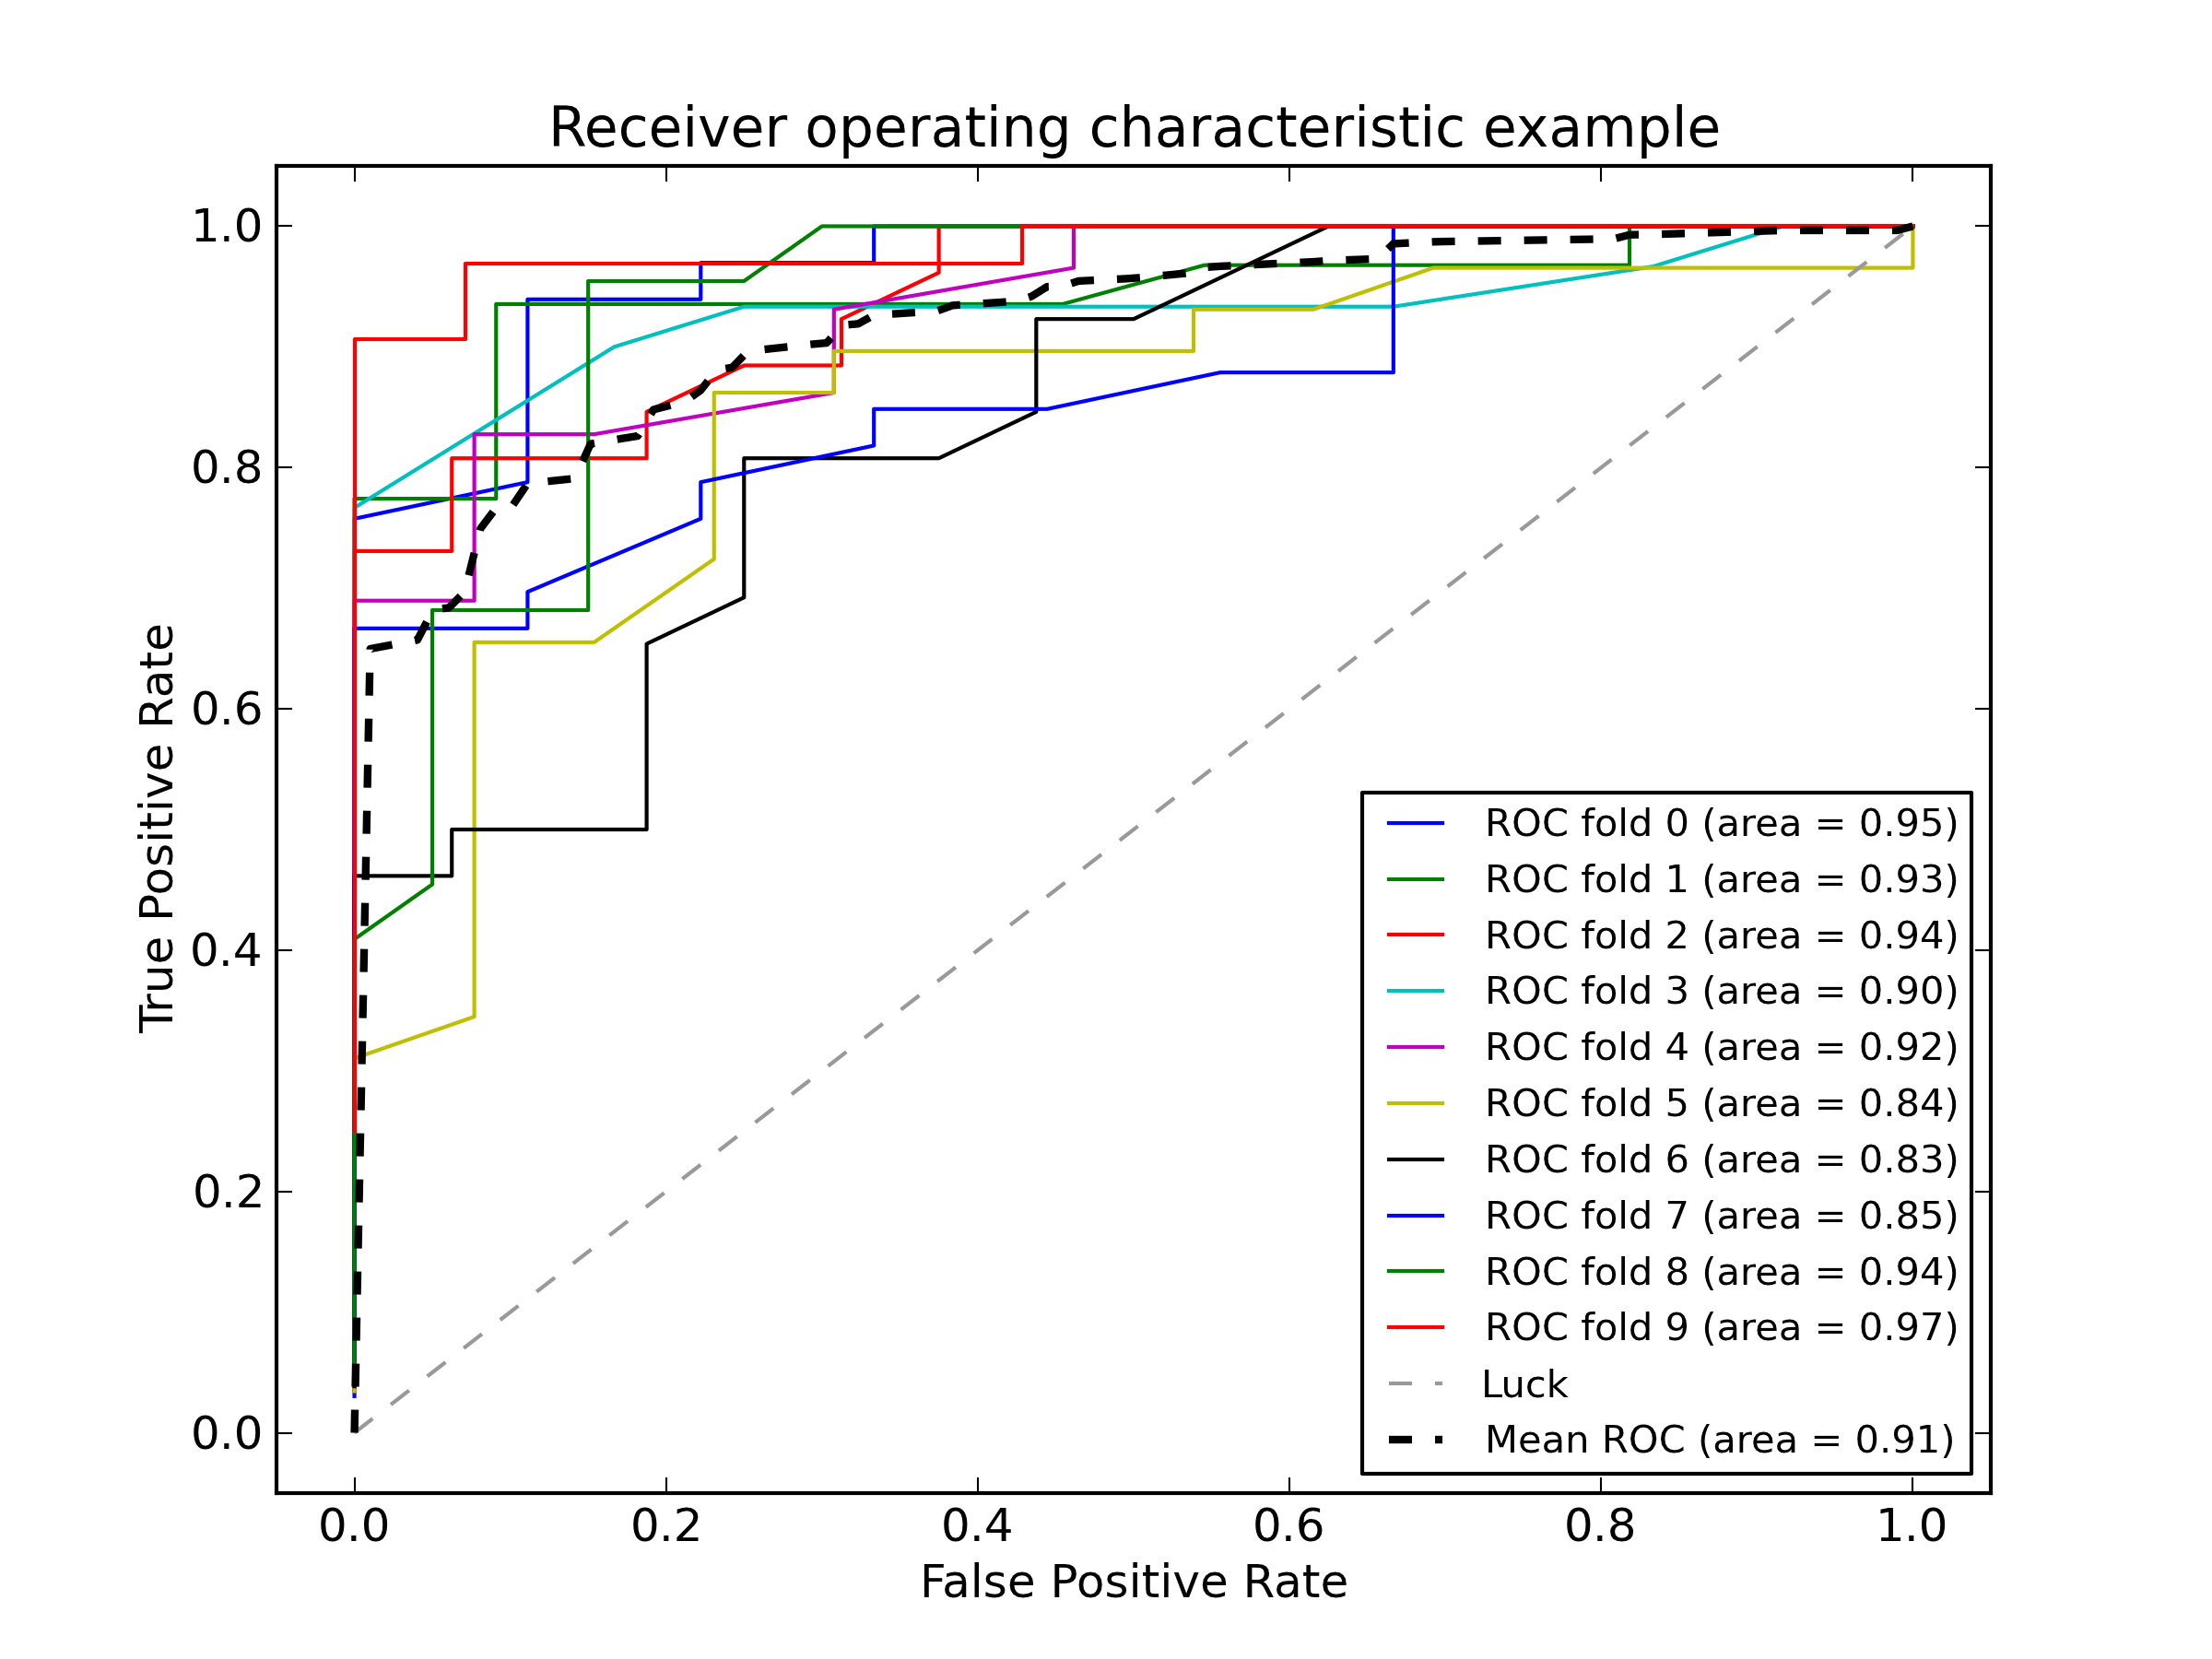
\includegraphics[width=0.36\textwidth]{pics/1_590_logit.png}}
\quad
\subfloat[Decision Trees]{
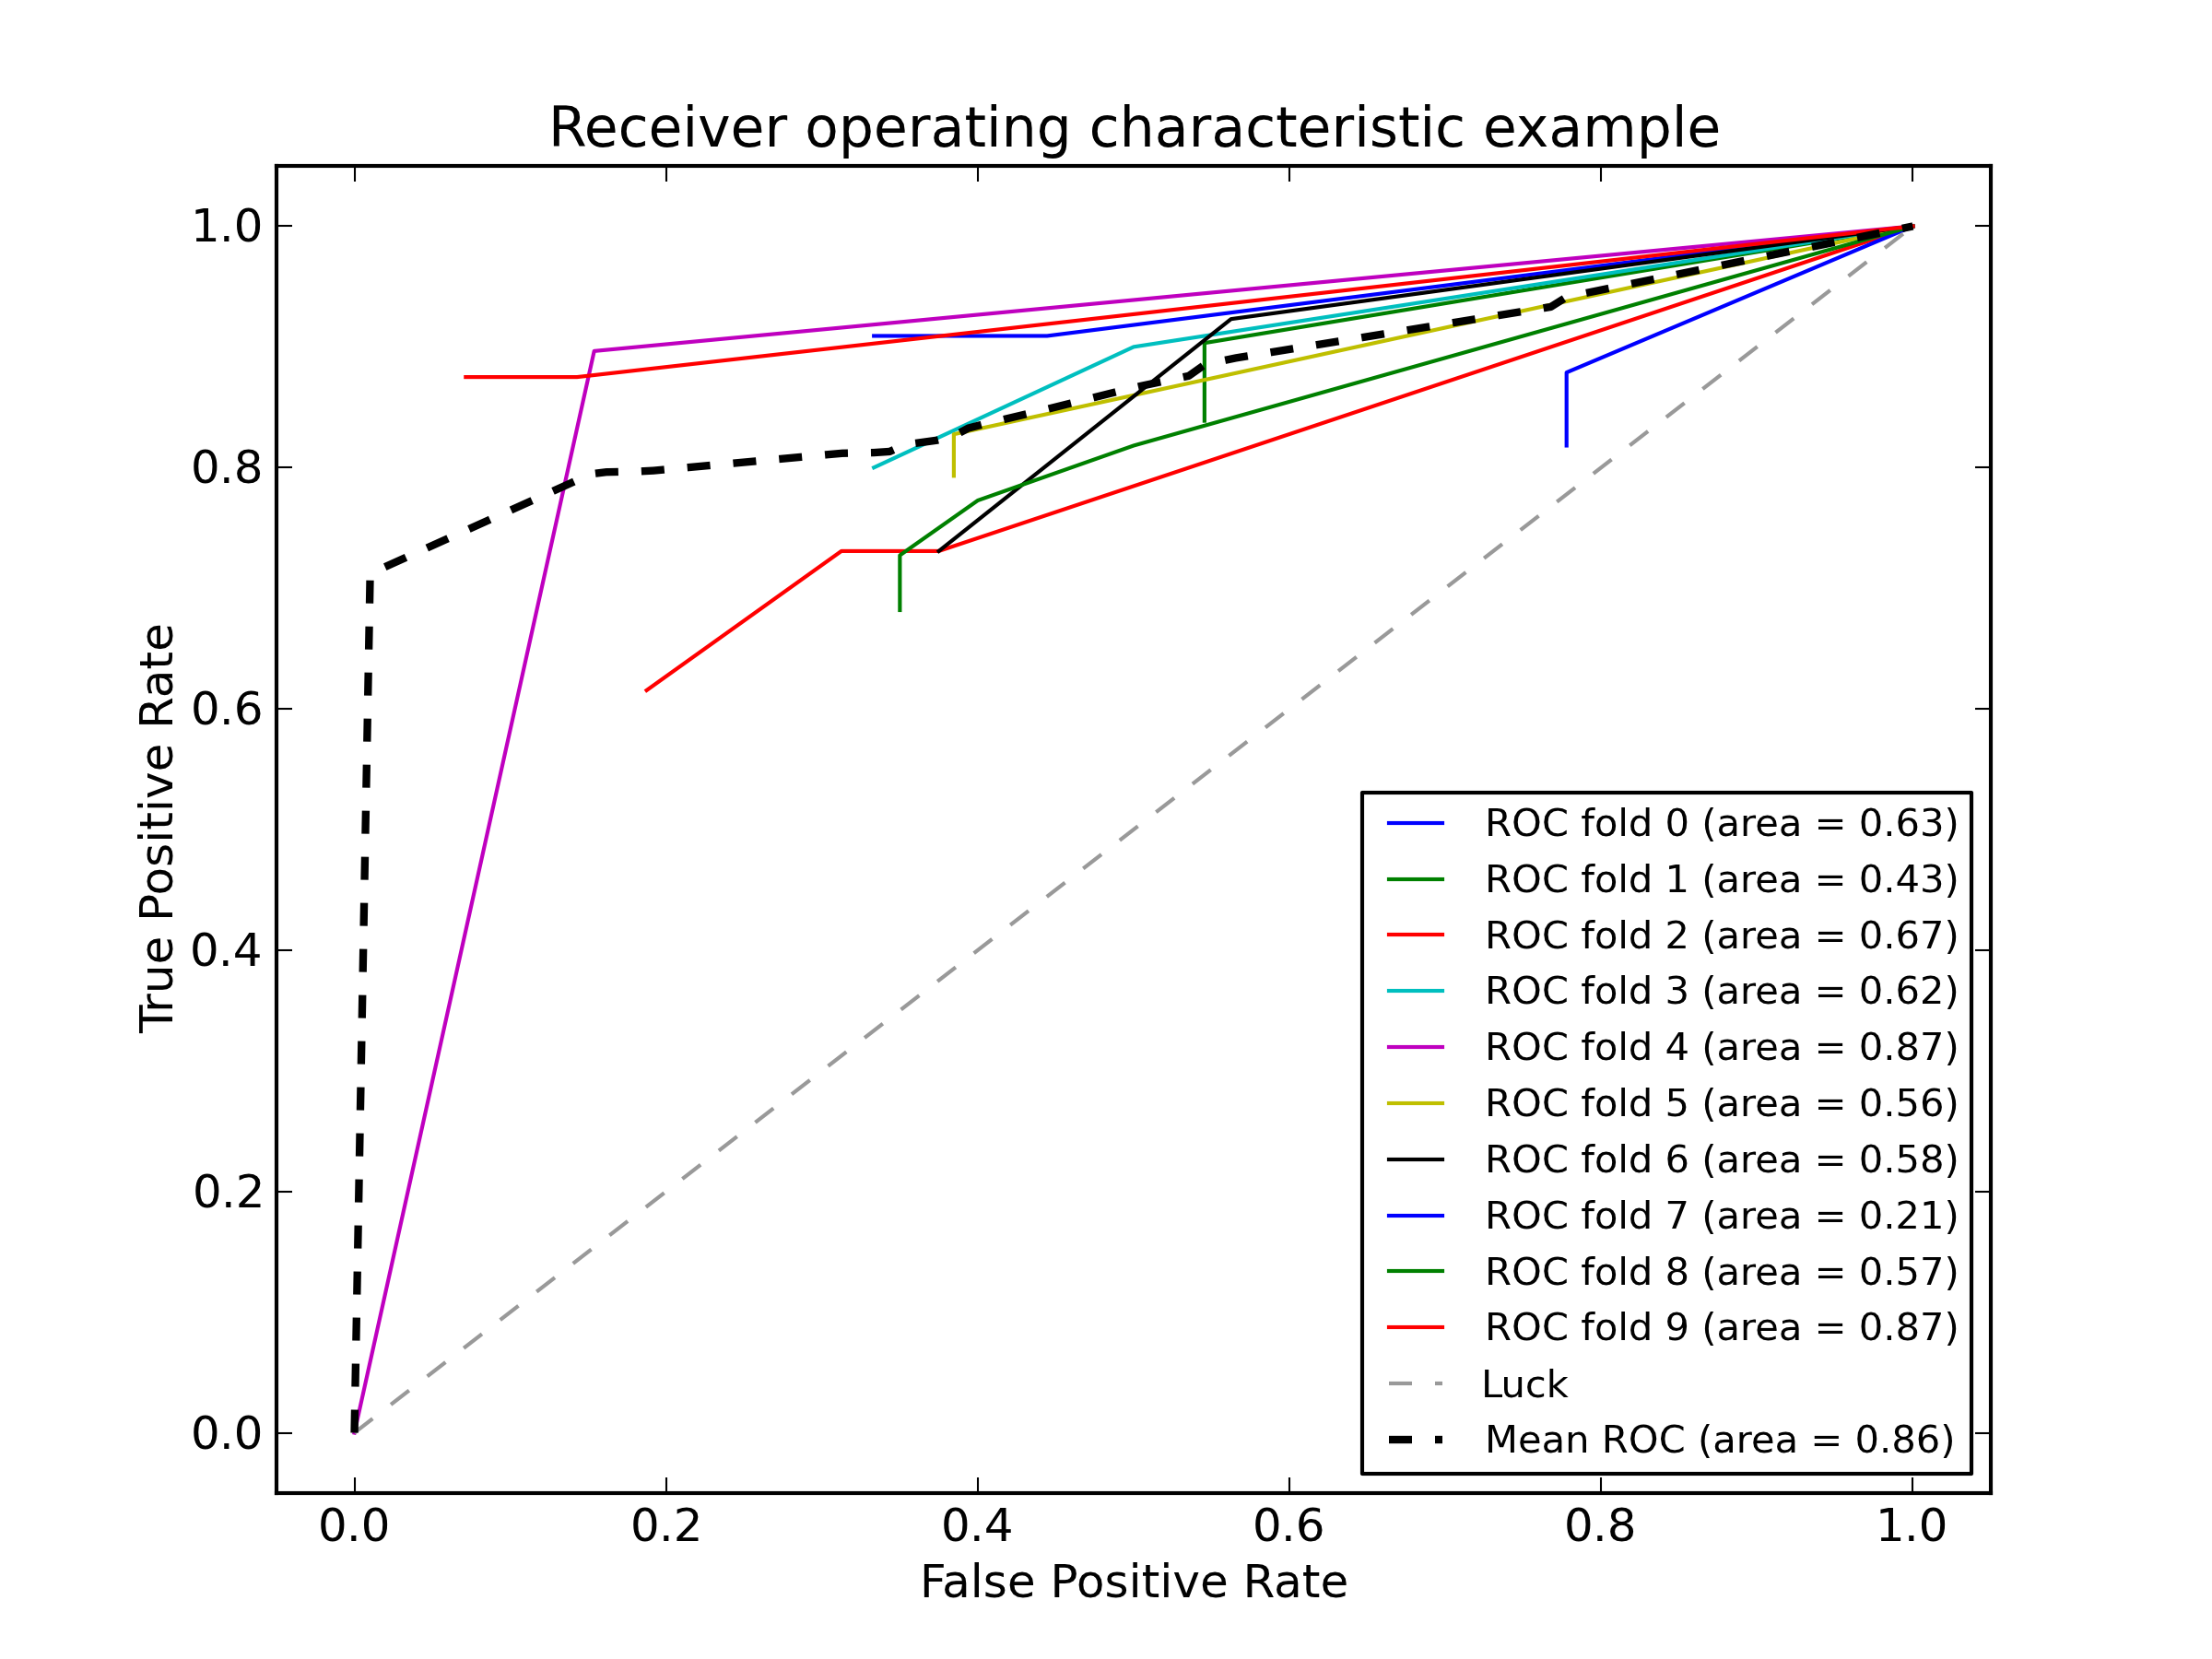
\includegraphics[width=0.36\textwidth]{pics/1_590_dtree.png}}
\quad
\subfloat[Multinomial Bayes]{
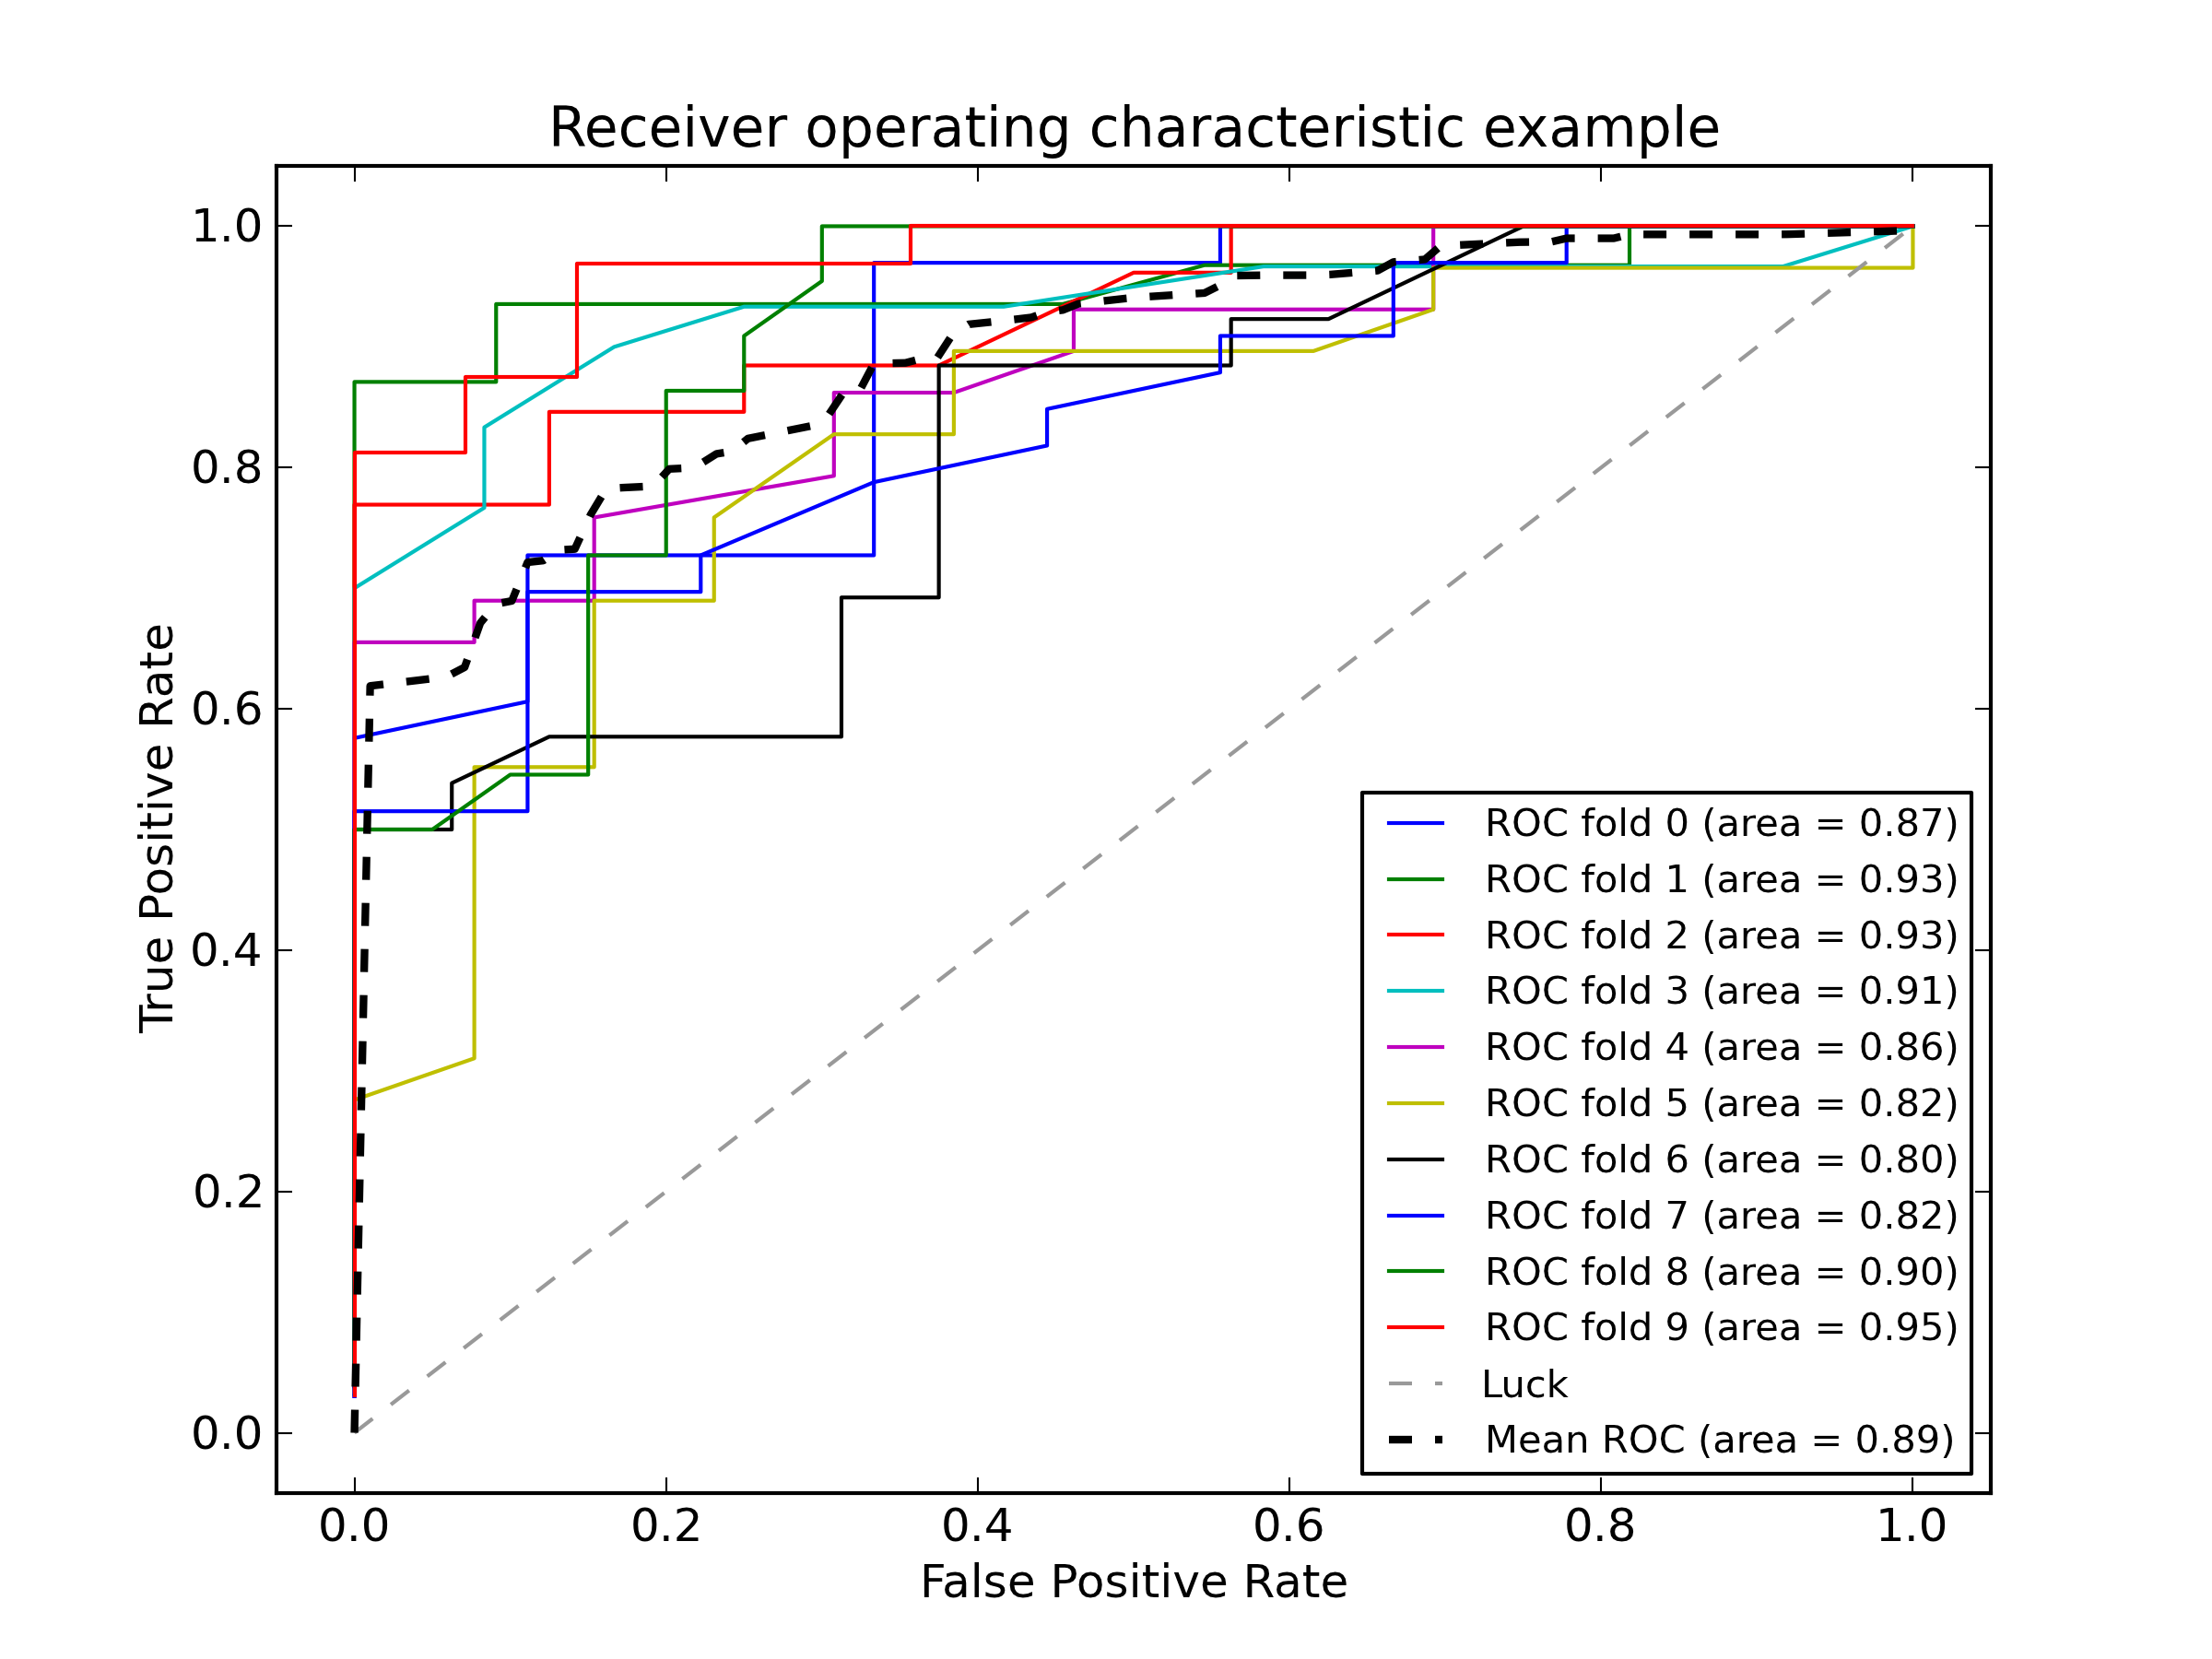
\includegraphics[width=0.36\textwidth]{pics/1_590_multi.png}}
\quad
\subfloat[Support Vector Machines]{
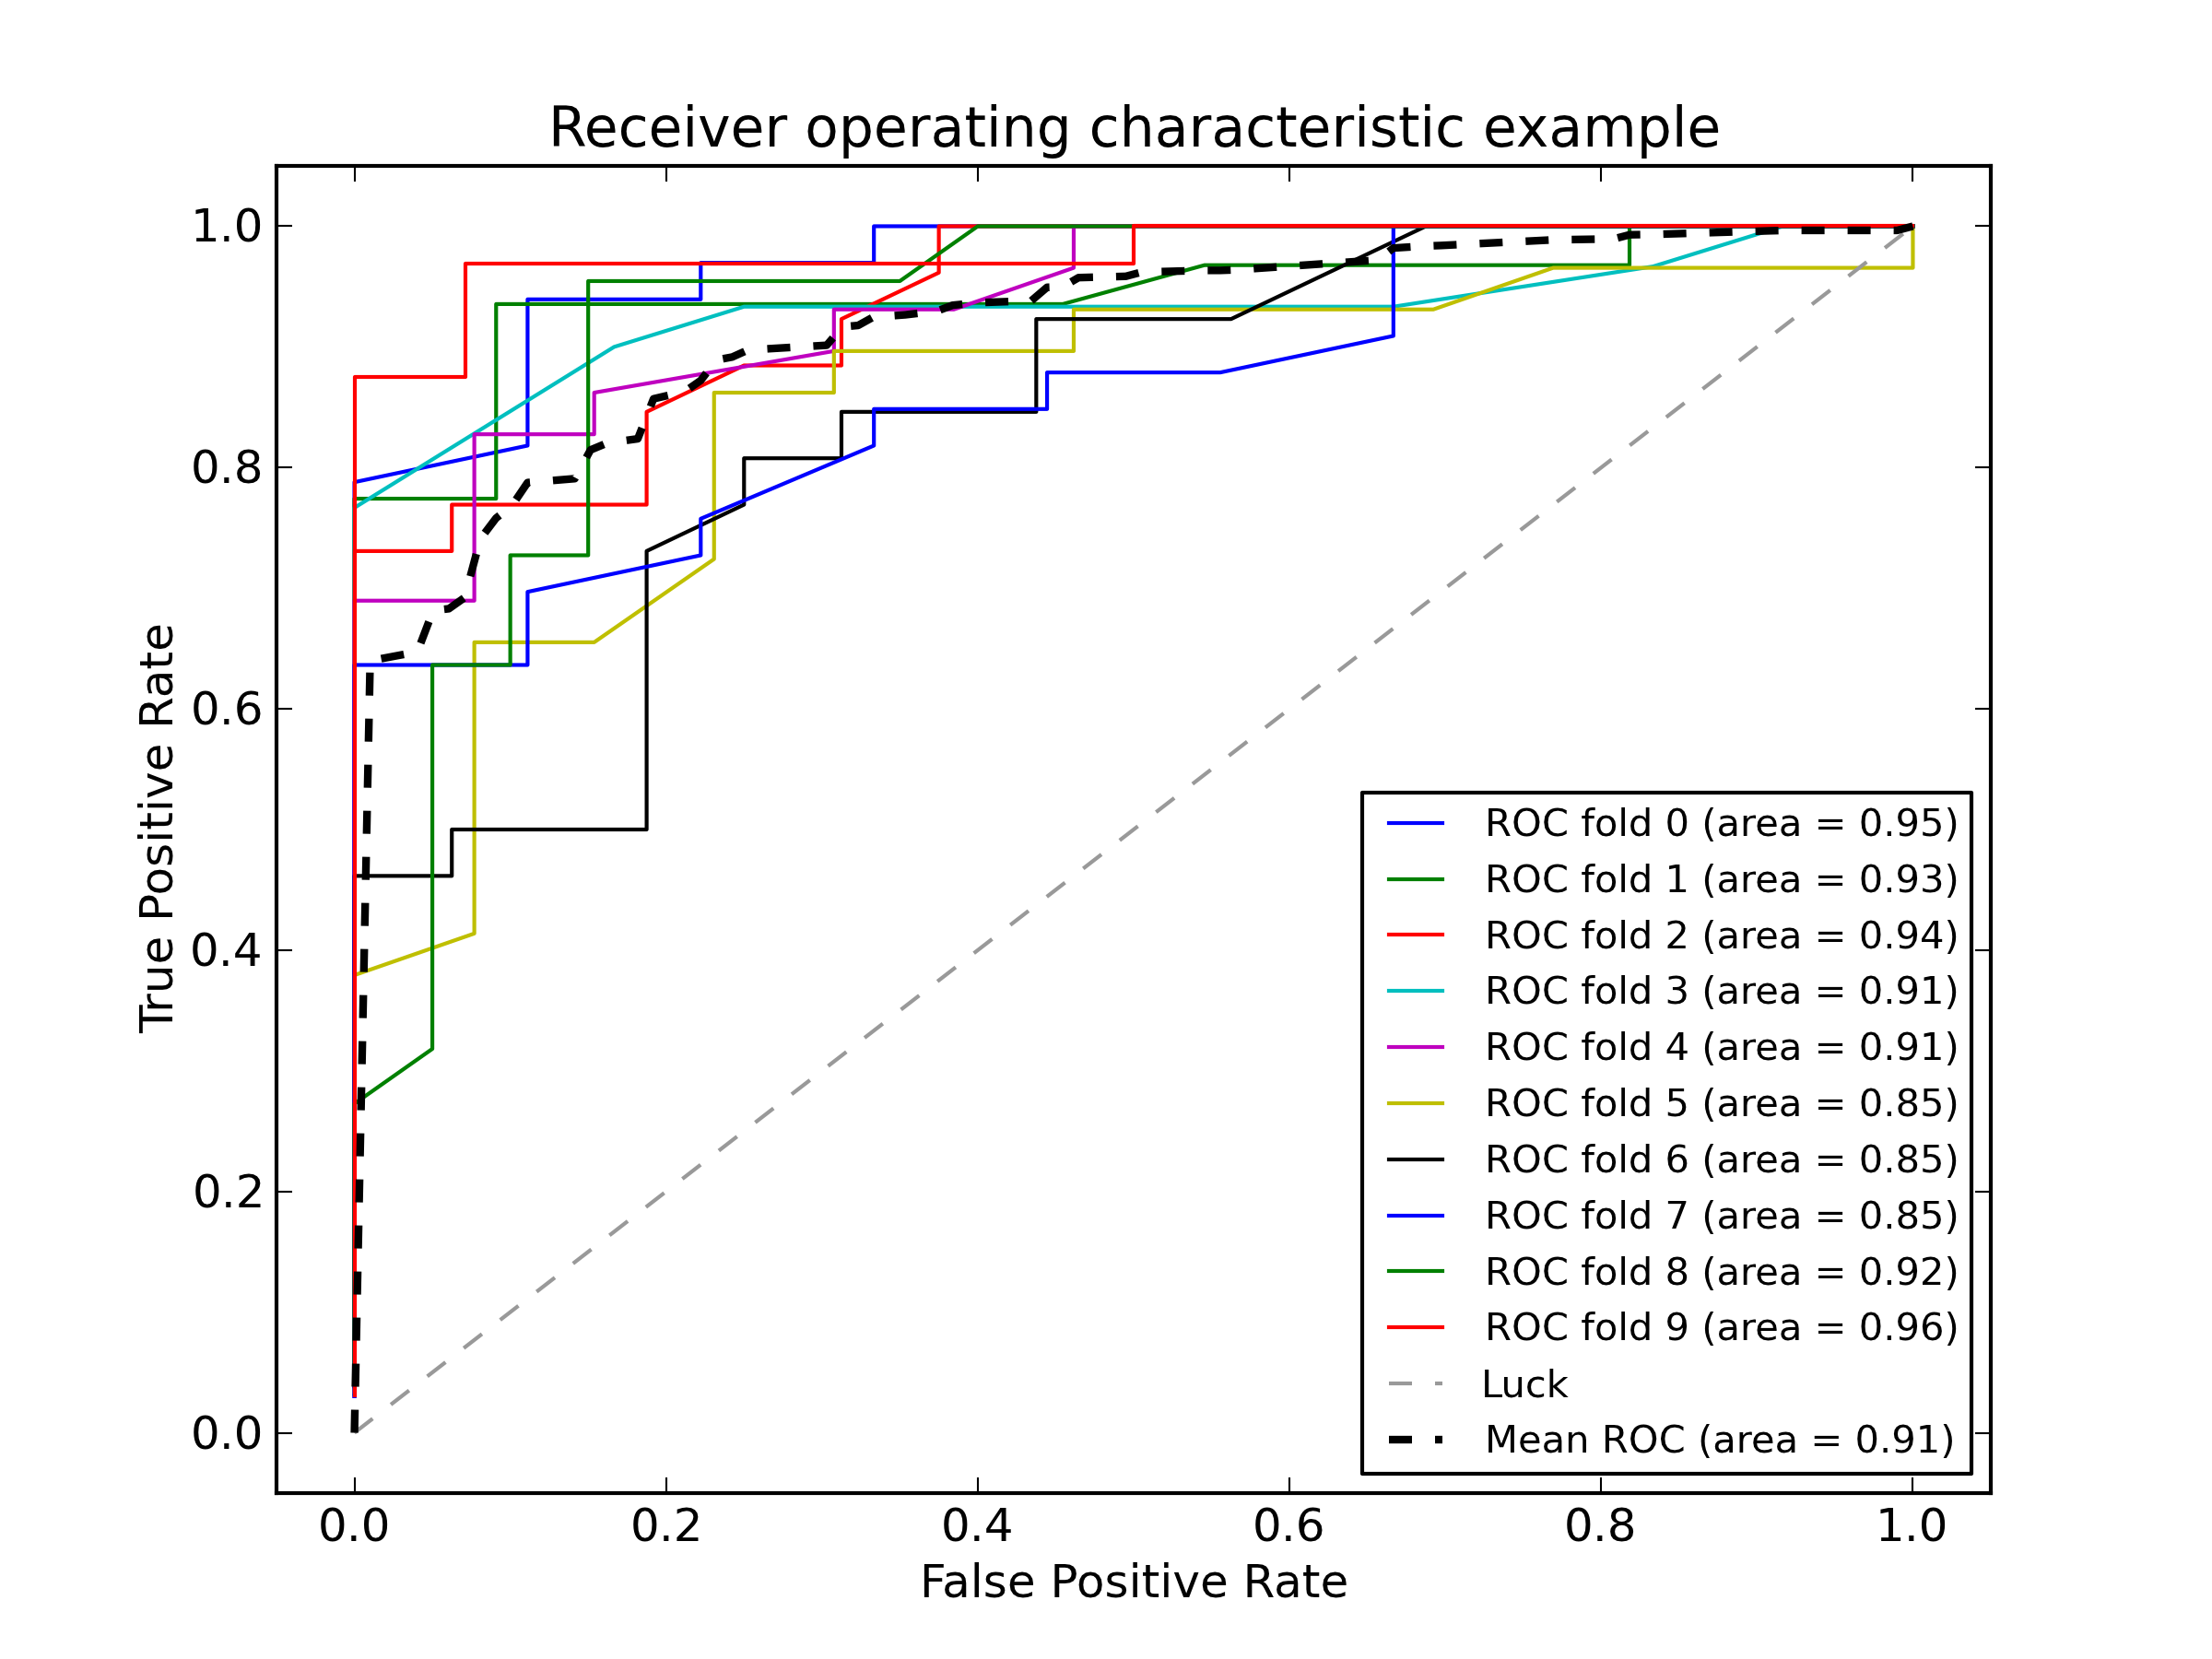
\includegraphics[width=0.36\textwidth]{pics/1_590_svm.png}}
\quad
\subfloat[Random Forests]{
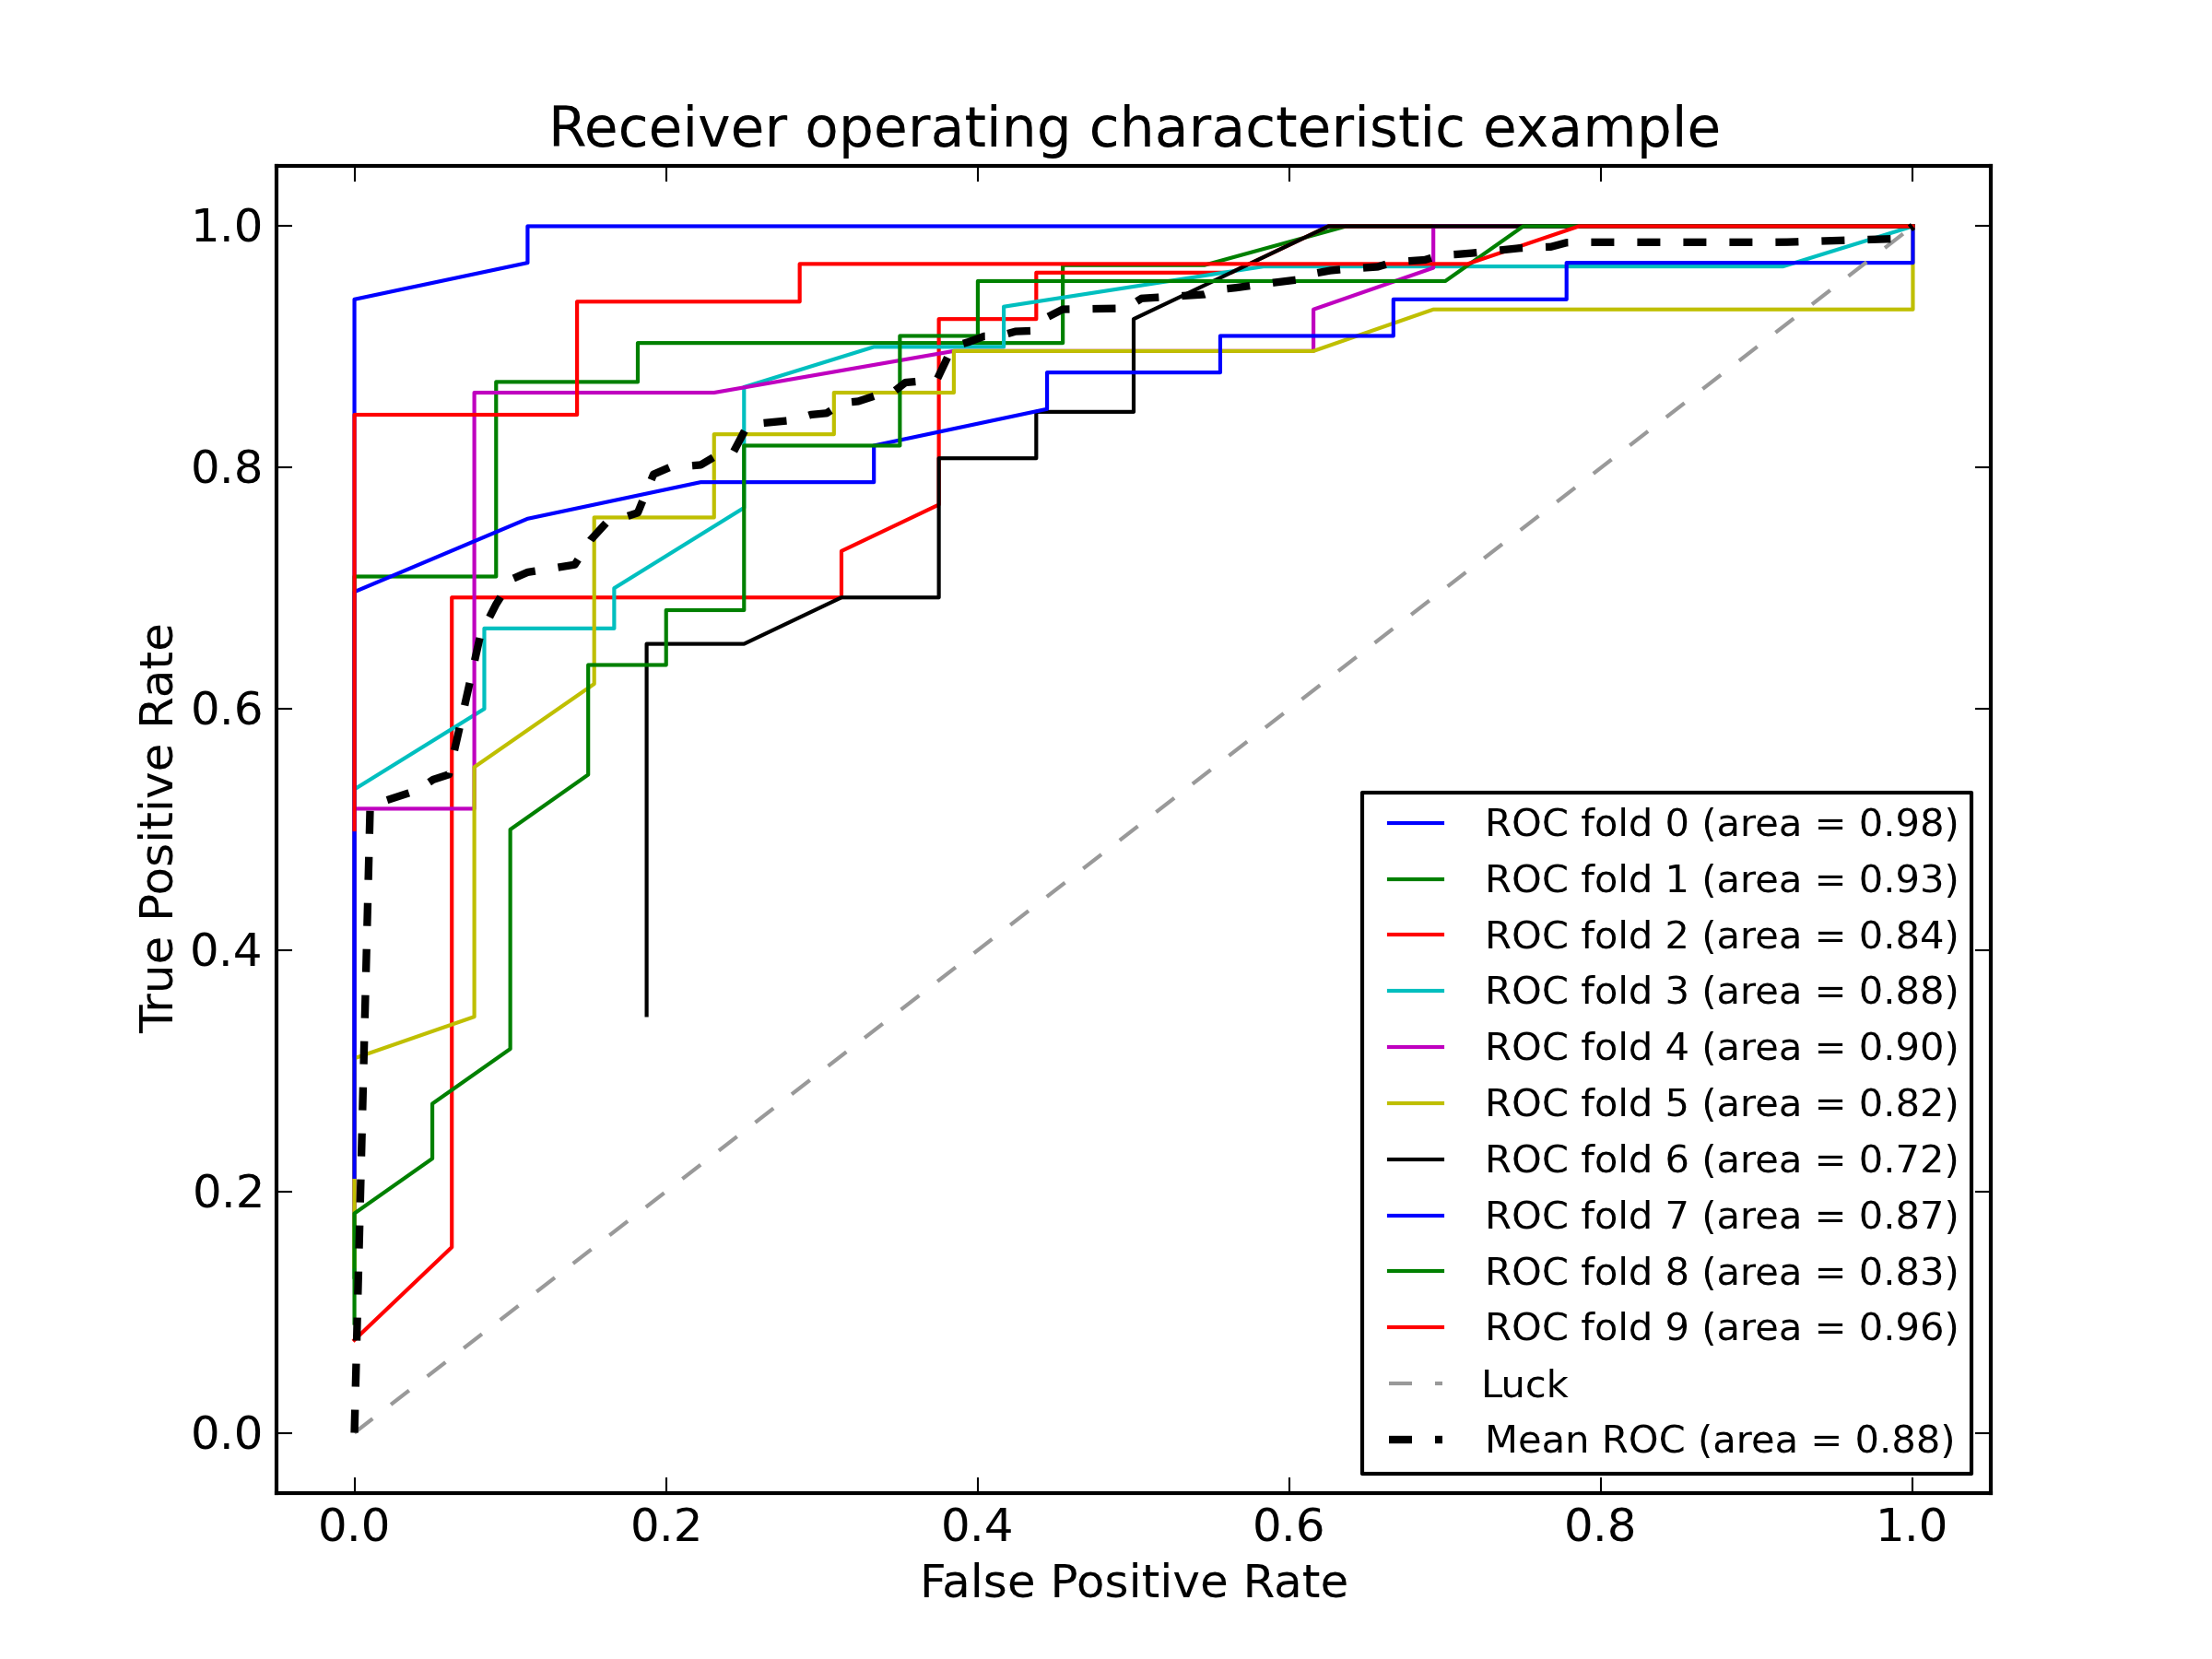
\includegraphics[width=0.36\textwidth]{pics/1_590_forest.png}}
\quad
\subfloat[Stacking - Logistic Regression]{
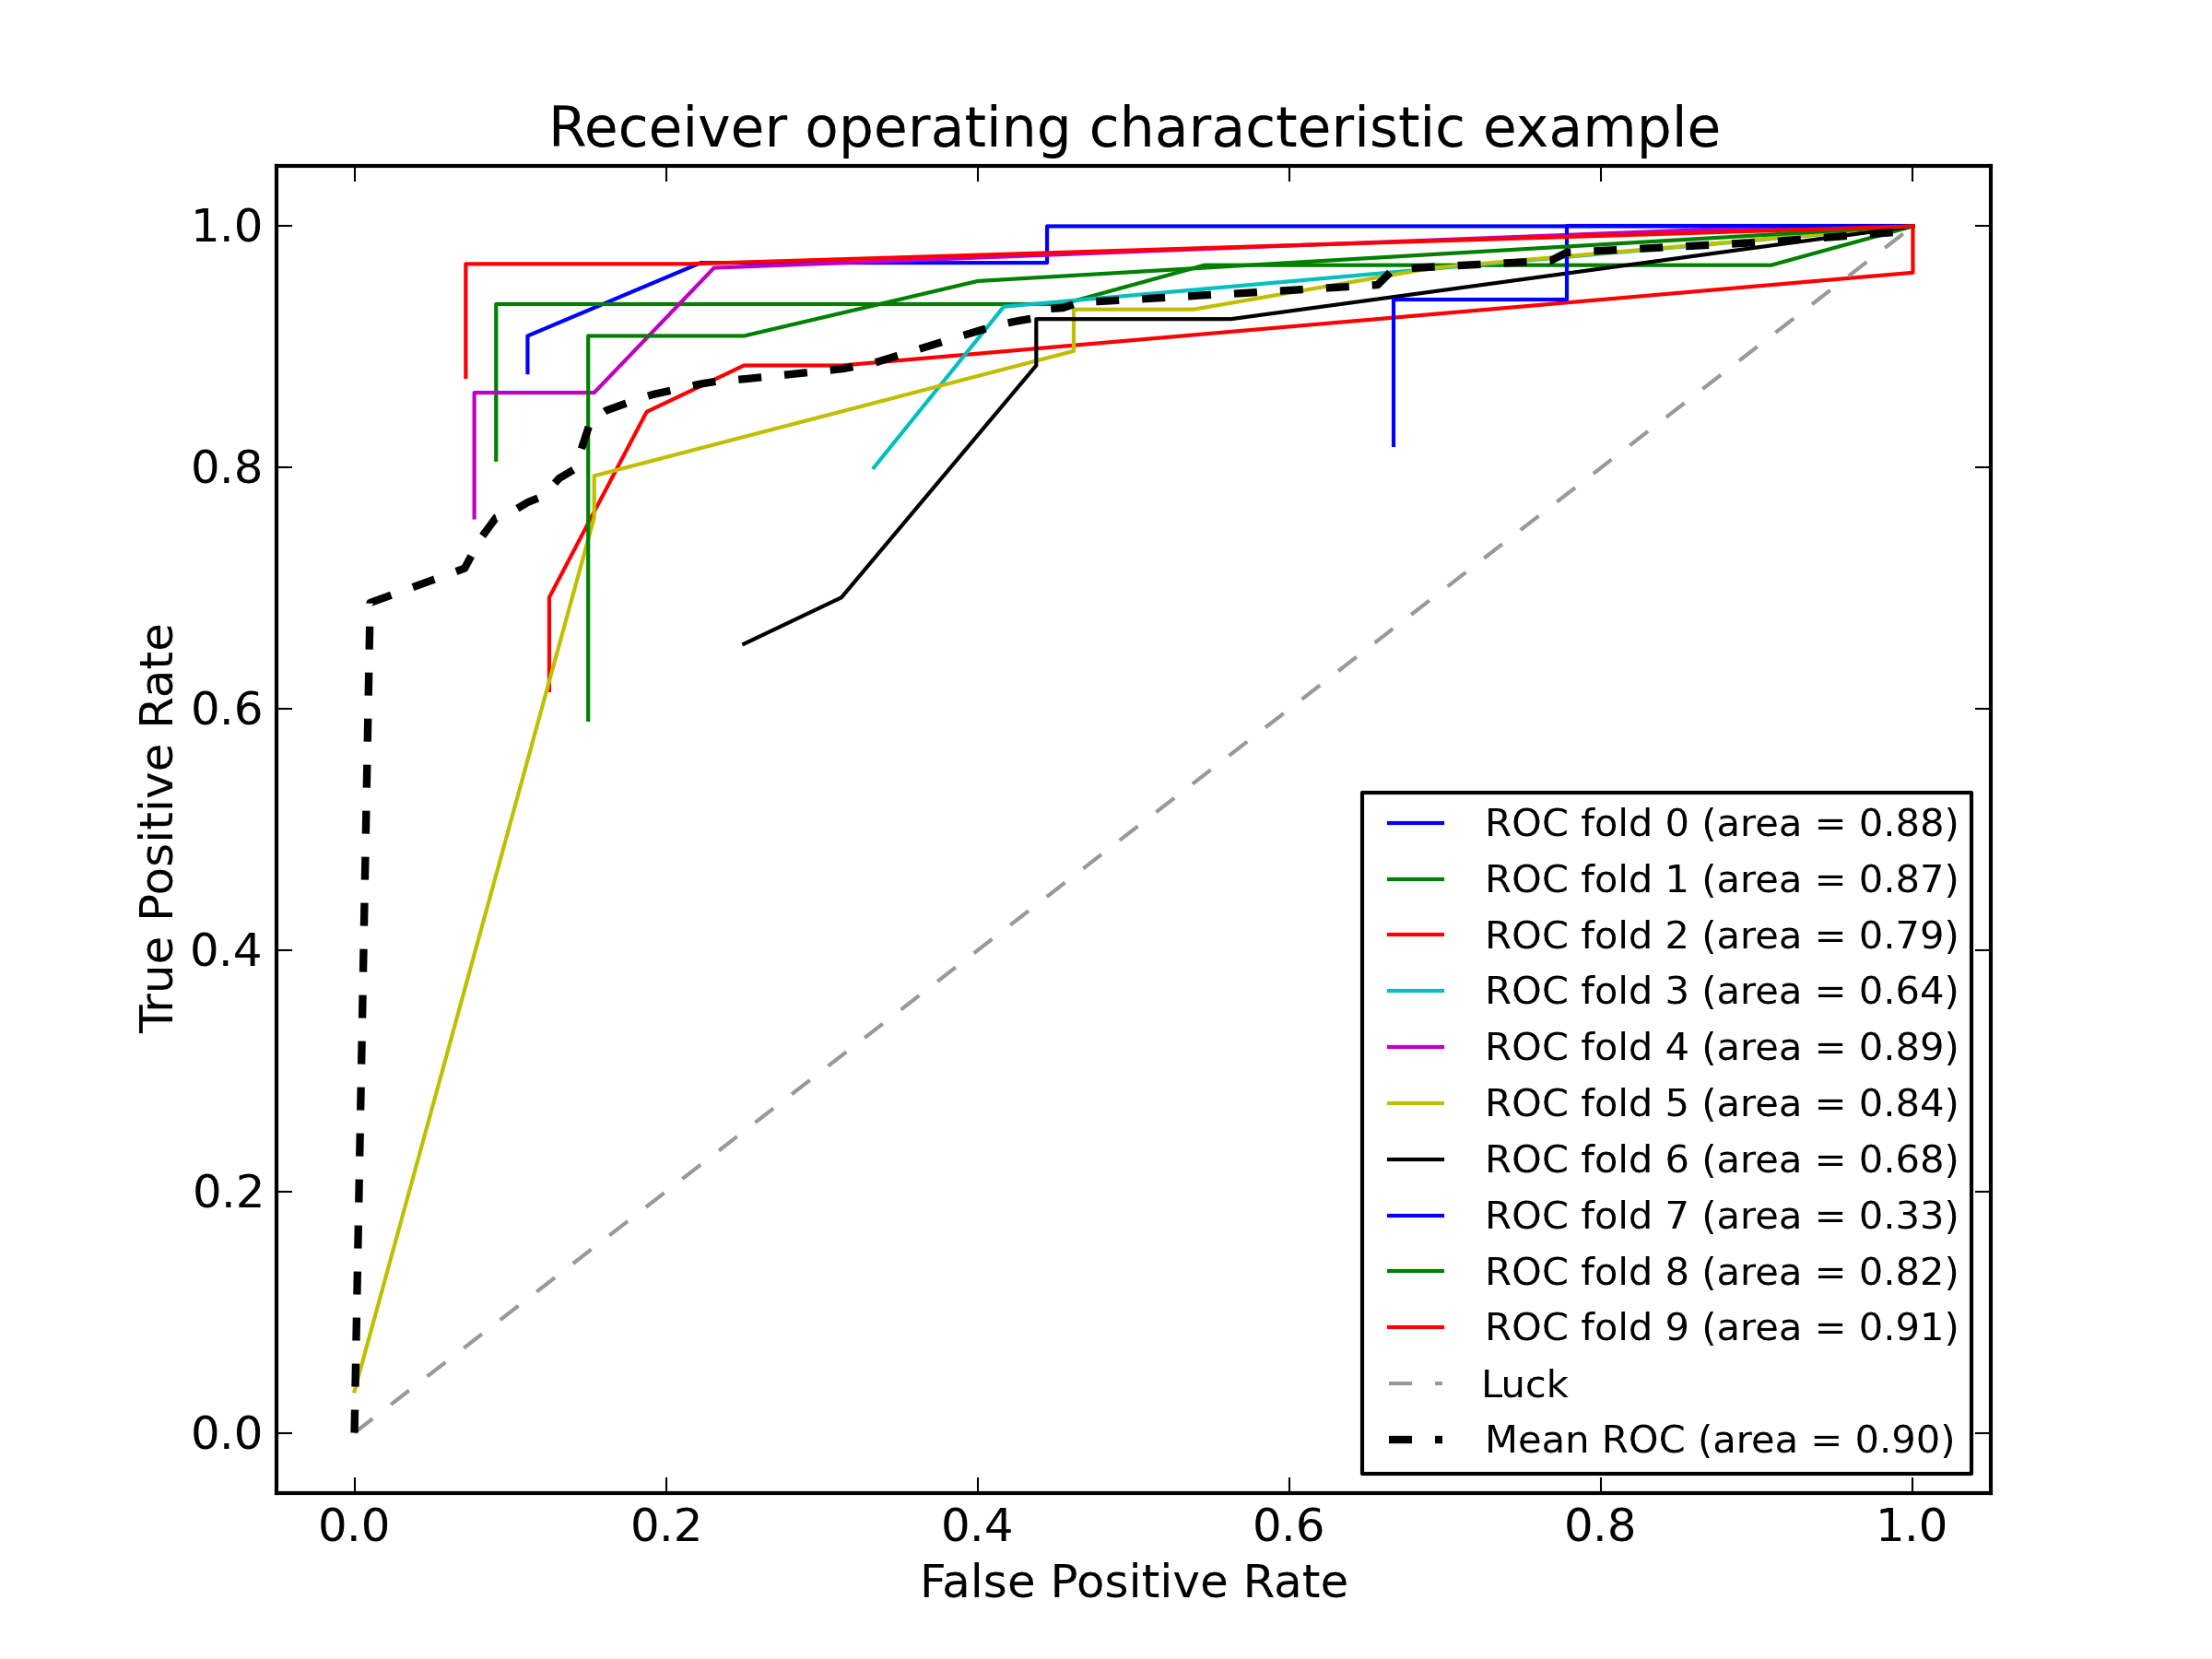
\includegraphics[width=0.36\textwidth]{pics/1_590_wmm.png}}
\quad
\subfloat[Stacking - Multi-Response Linear Models]{
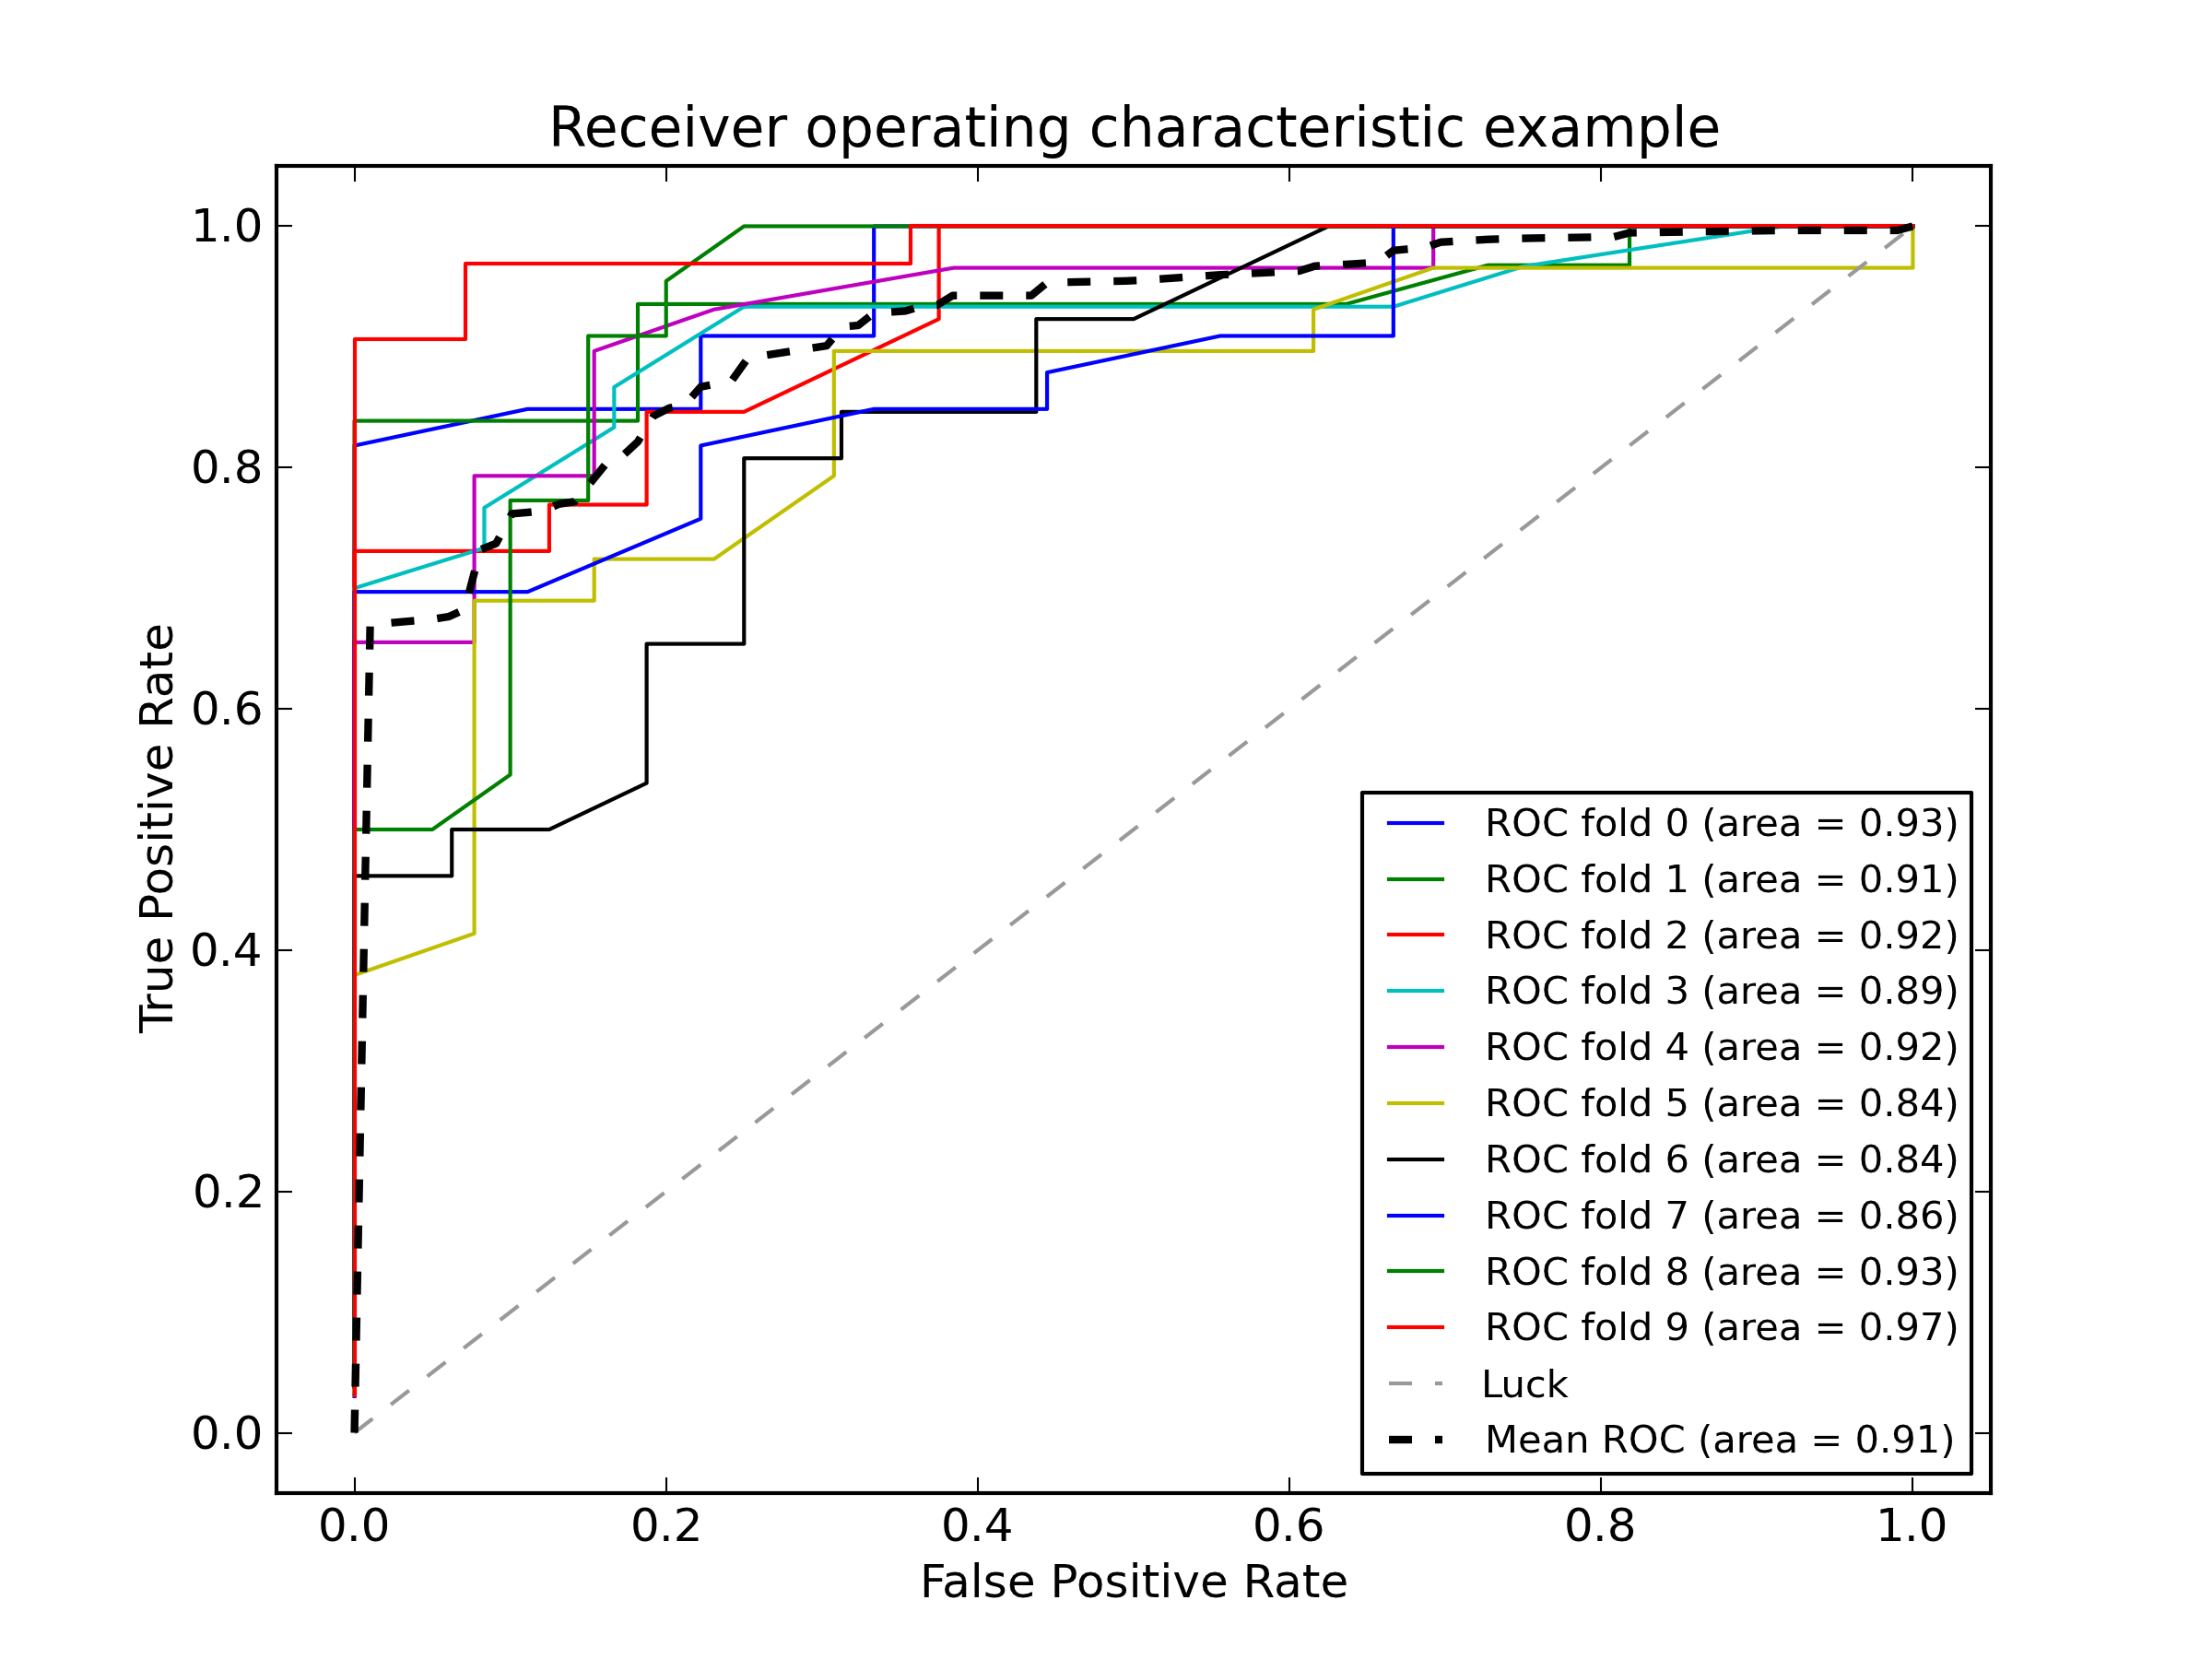
\includegraphics[width=0.36\textwidth]{pics/1_590_smm.png}}
\caption{Results for Features 1-8}
\label{fig:fig2}
\end{figure}

\begin{figure}[t]
\centering
\subfloat[Logistic Regression]{
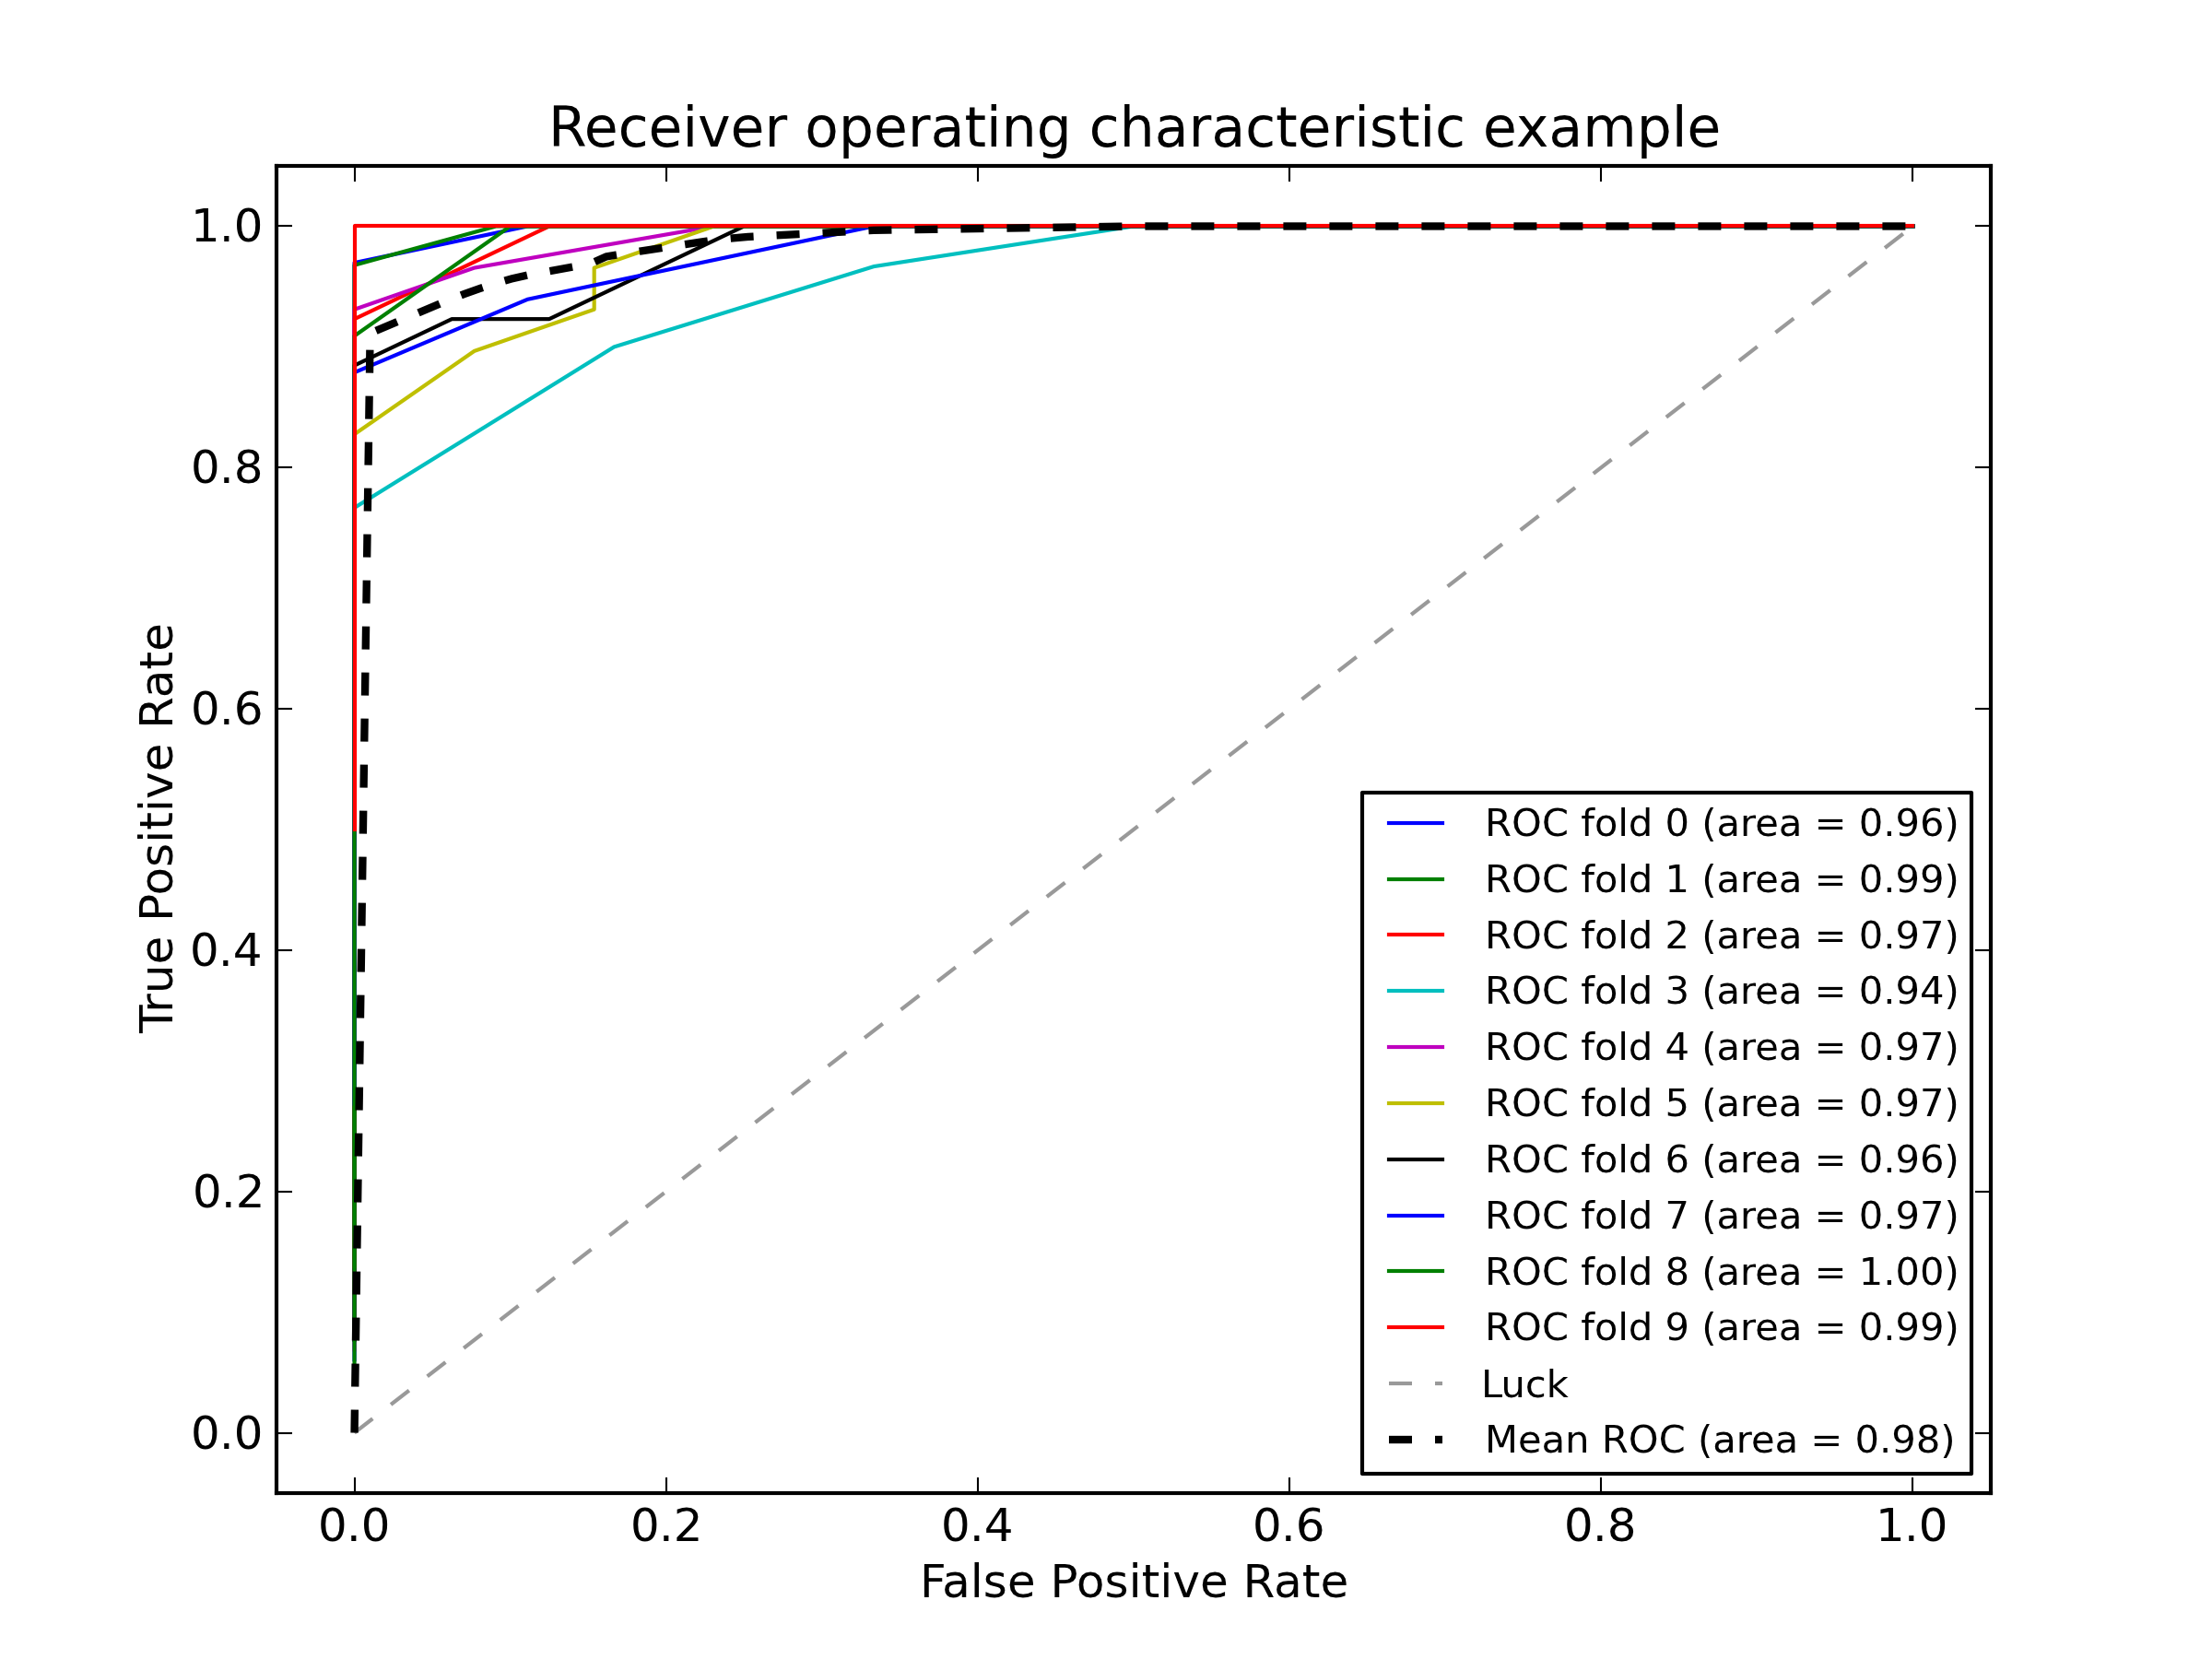
\includegraphics[width=0.36\textwidth]{pics/2_590_logit.png}}
\quad
\subfloat[Decision Trees]{
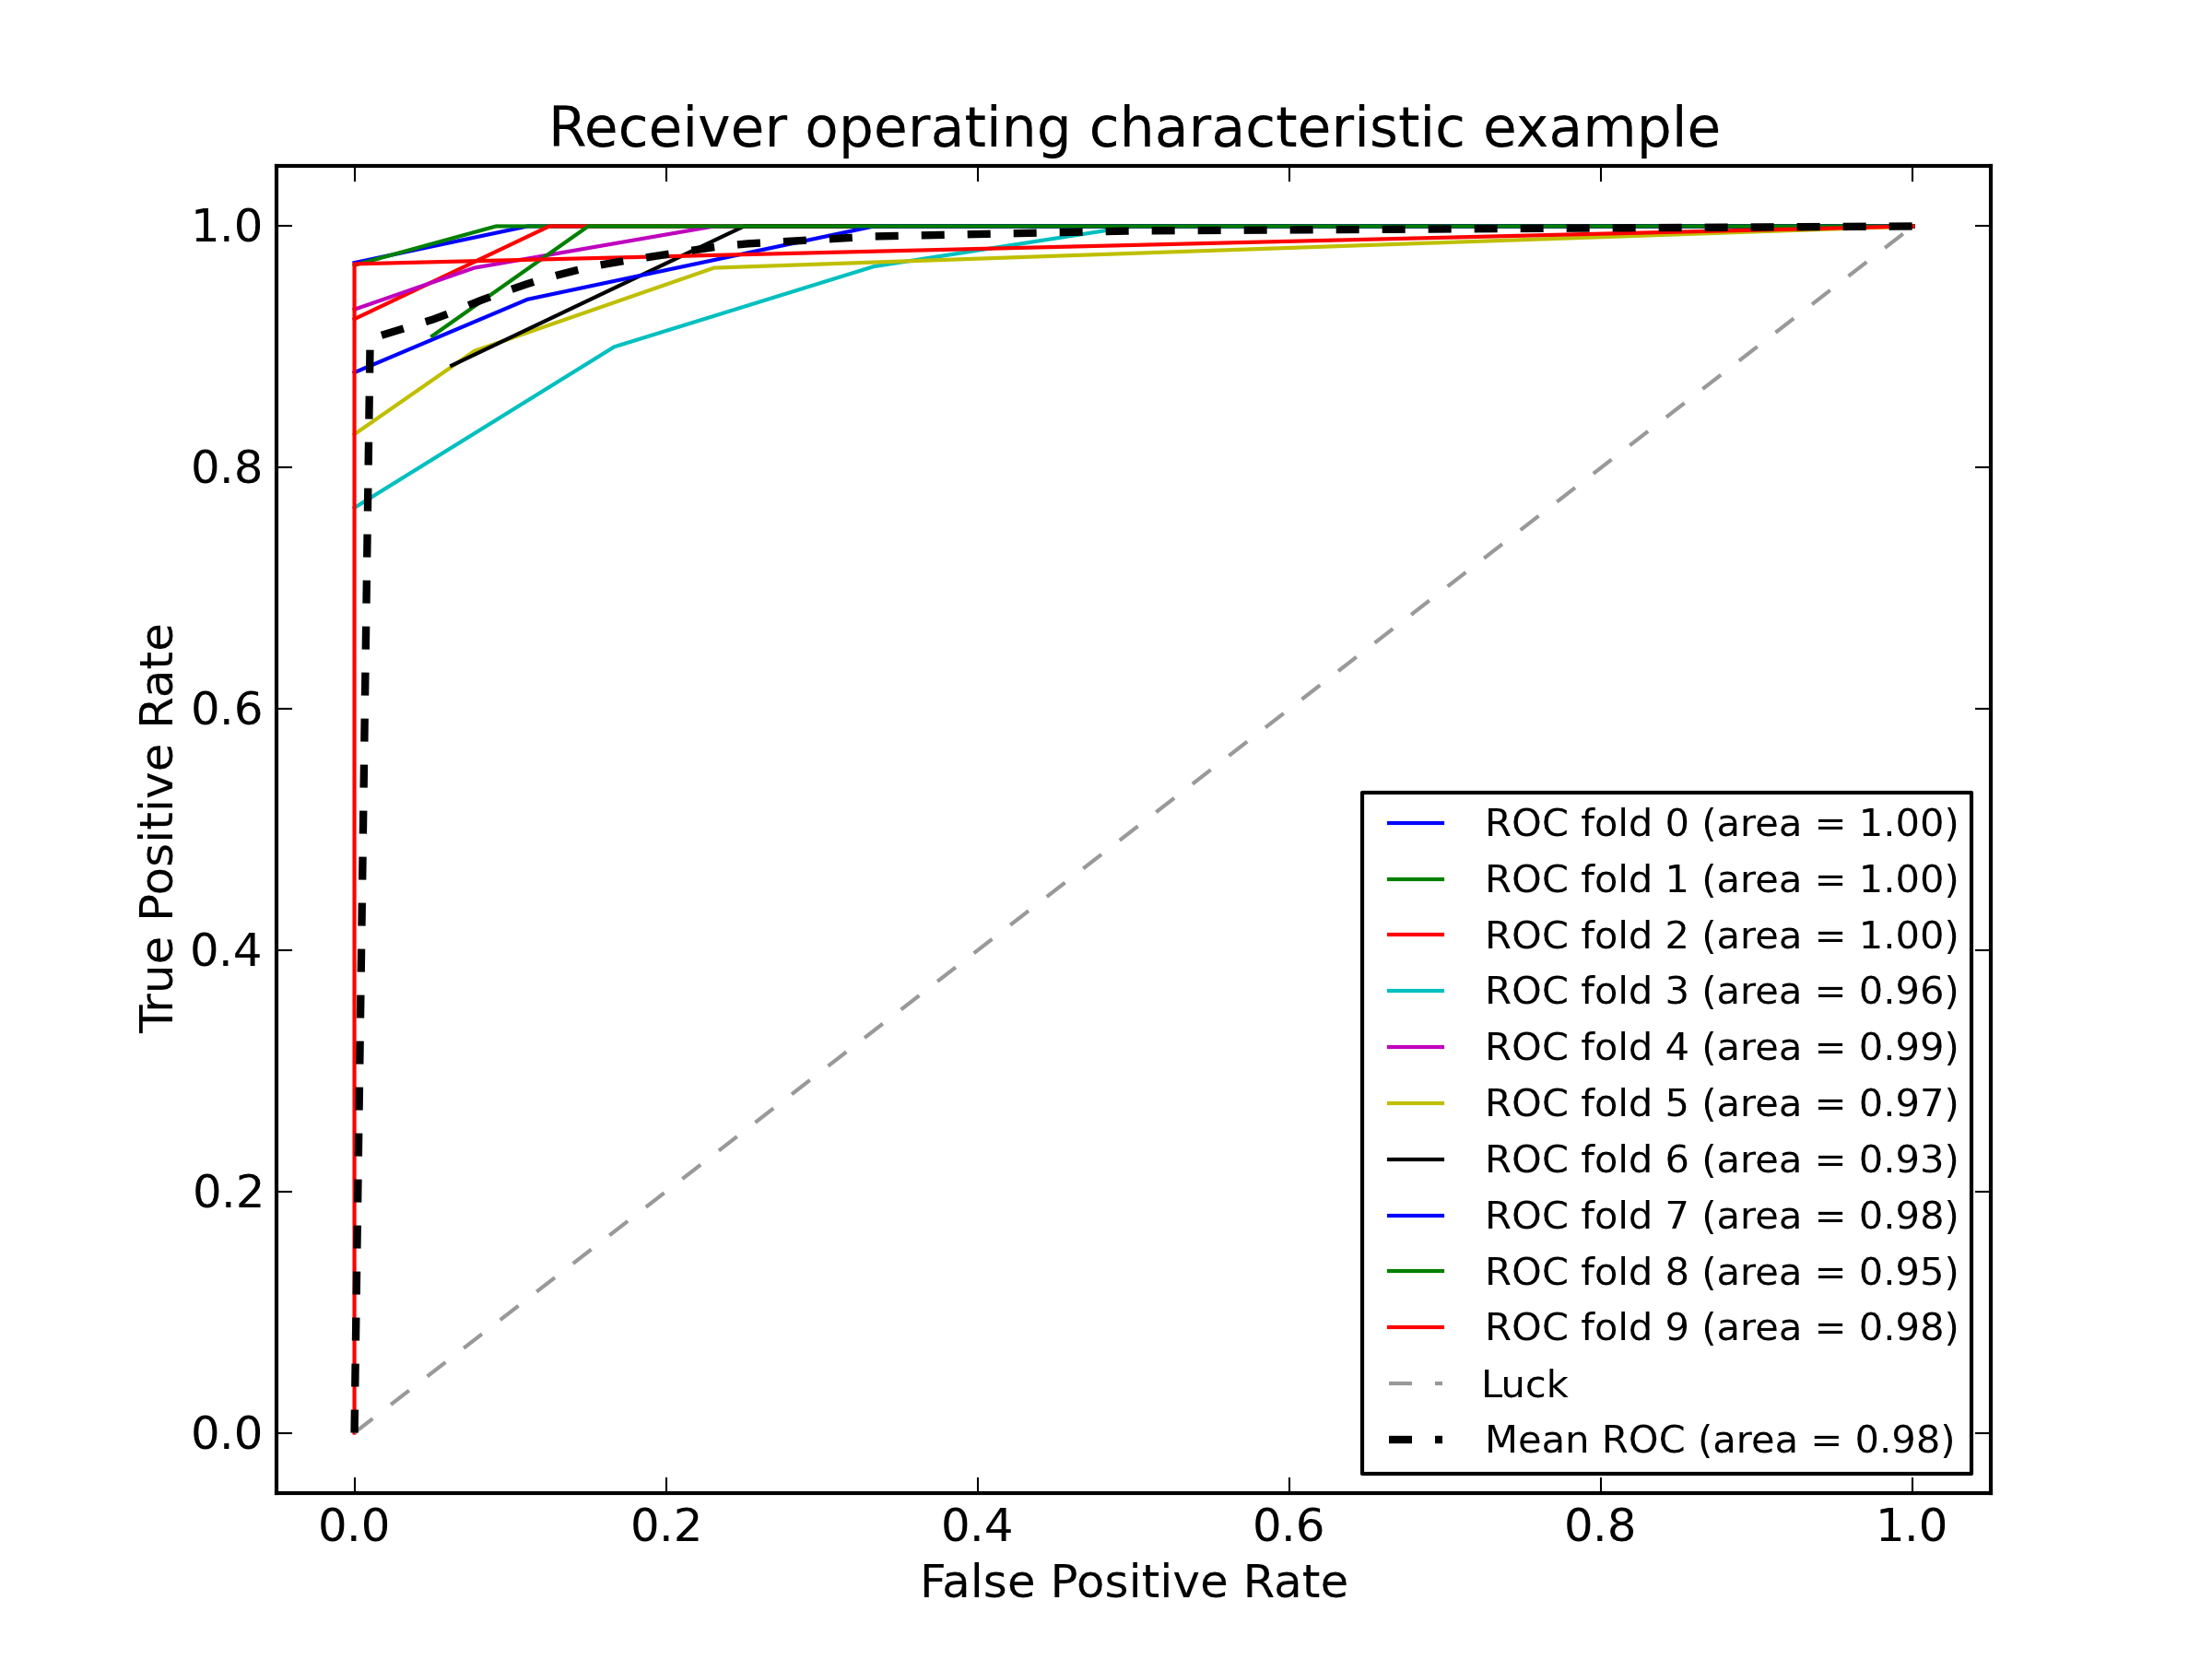
\includegraphics[width=0.36\textwidth]{pics/2_590_dtree.png}}
\quad
\subfloat[Multinomial Bayes]{
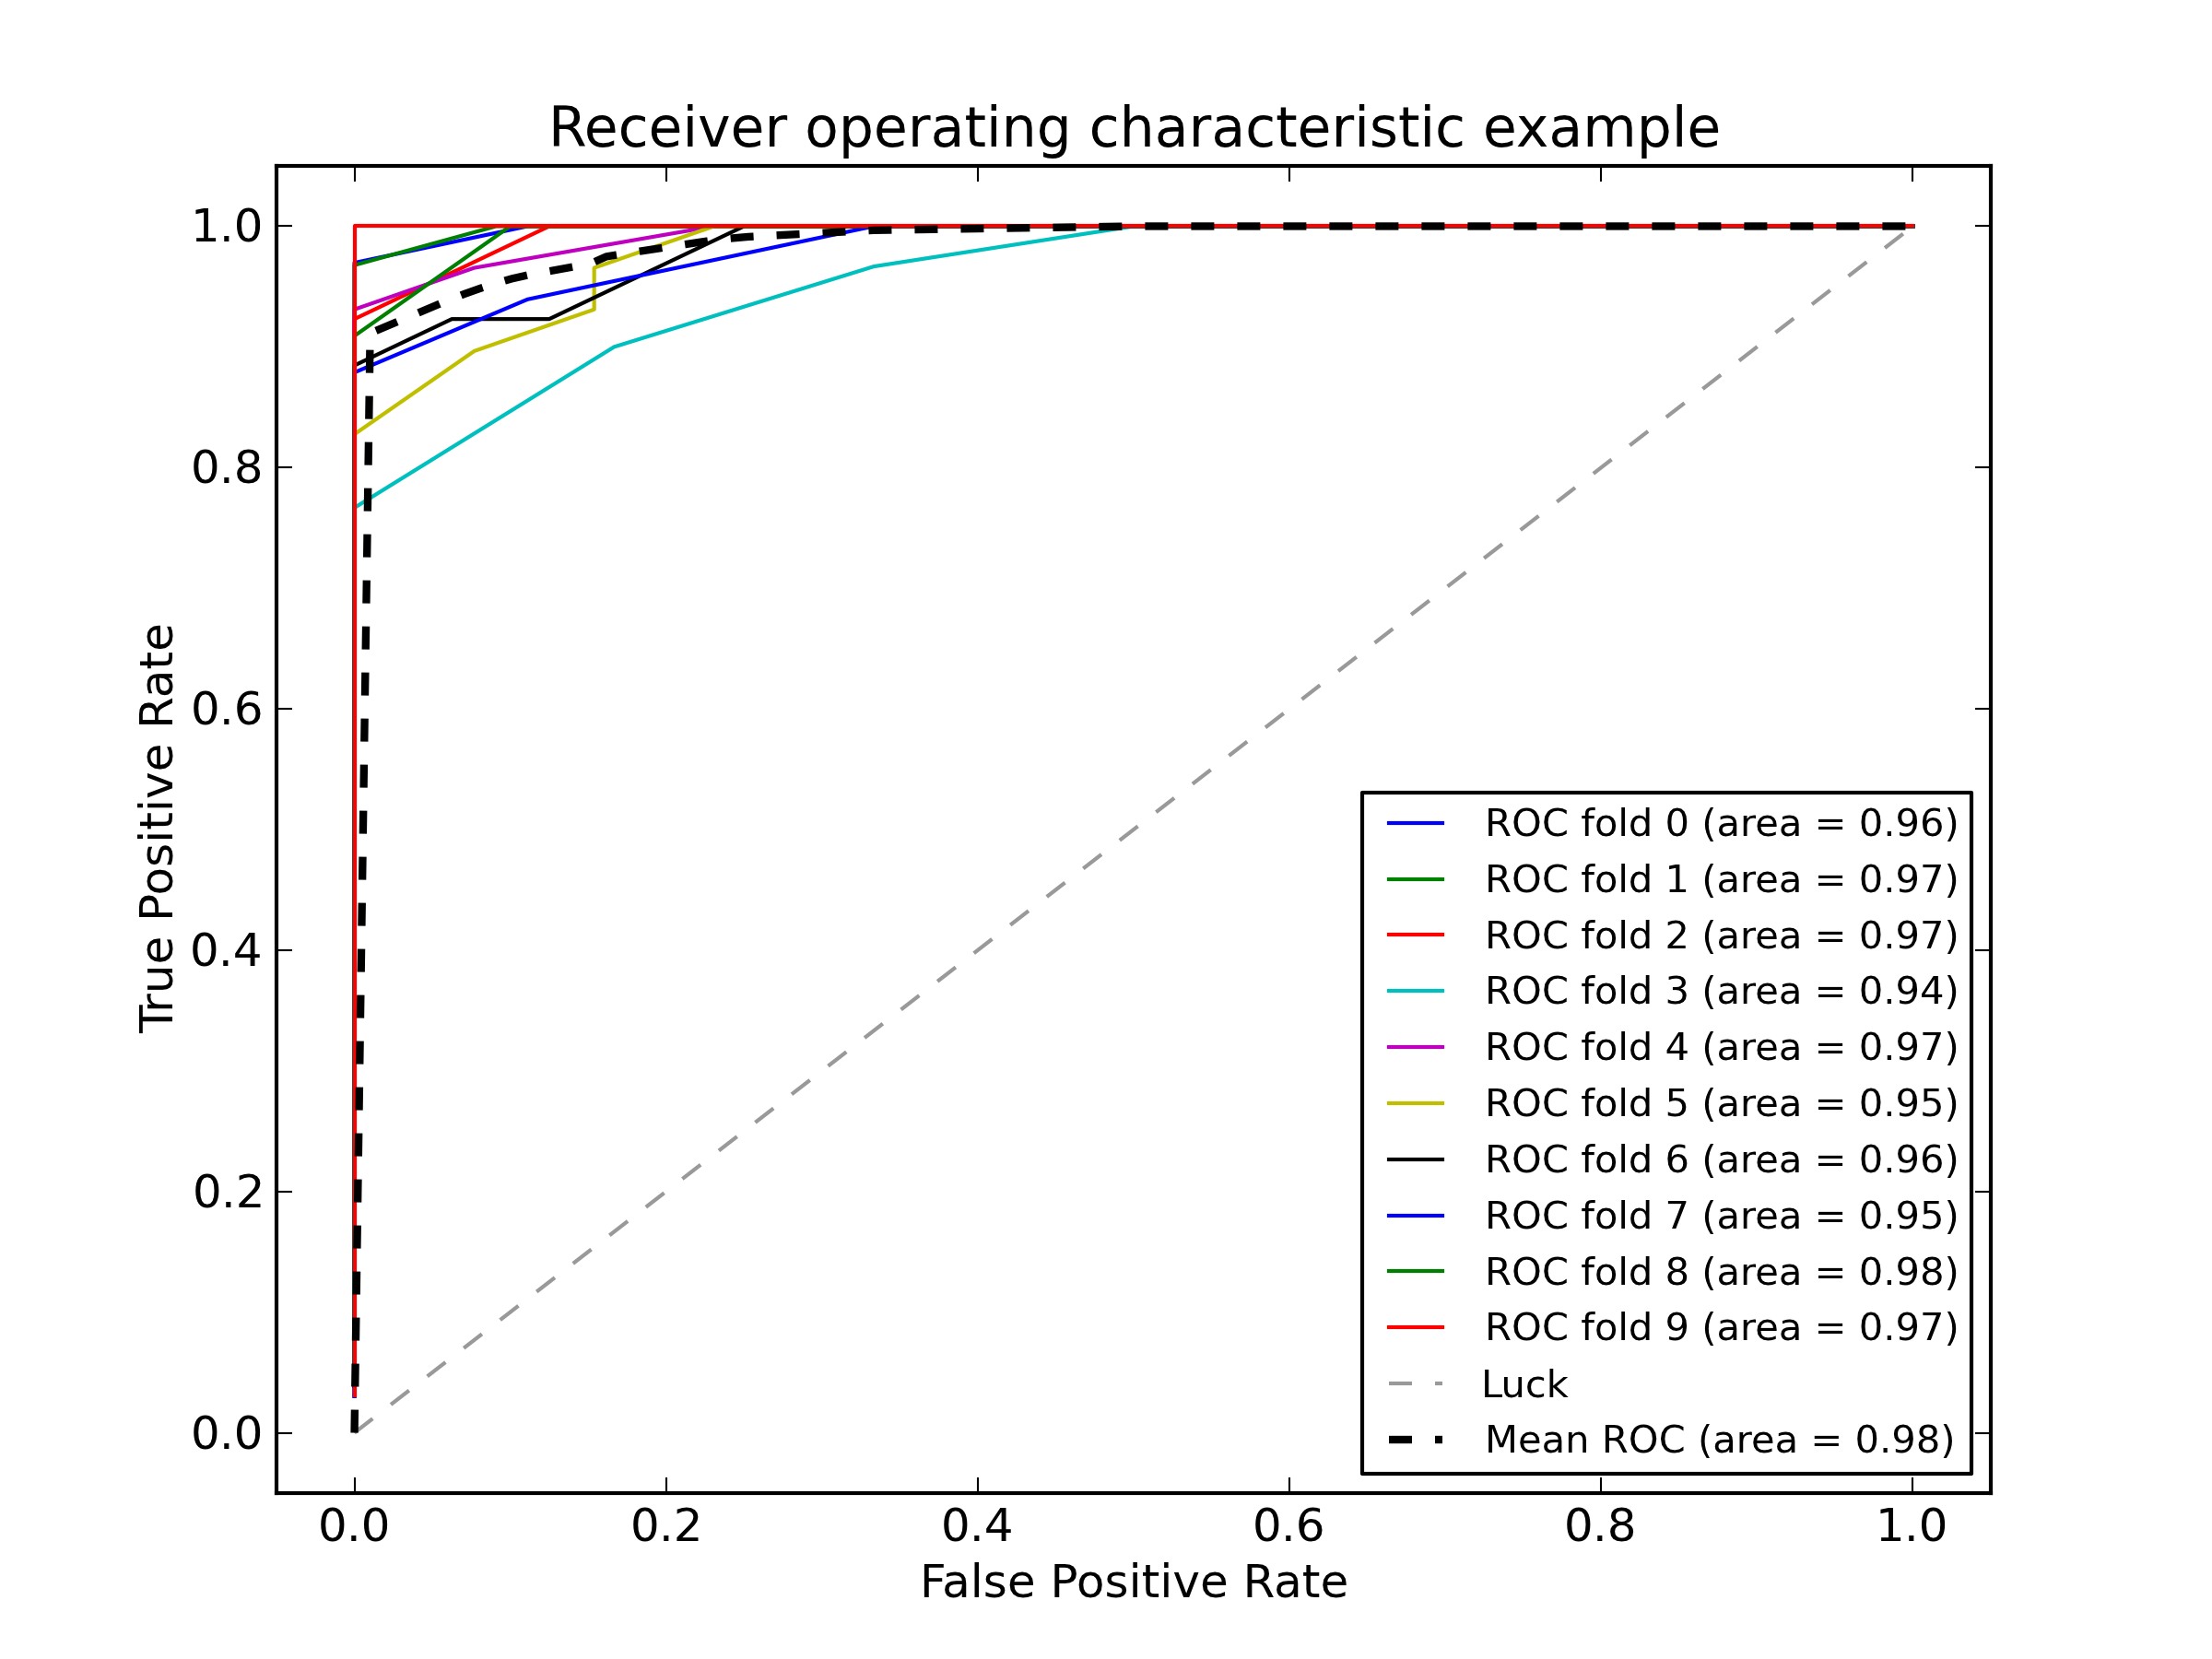
\includegraphics[width=0.36\textwidth]{pics/2_590_multi.png}}
\quad
\subfloat[Support Vector Machines]{
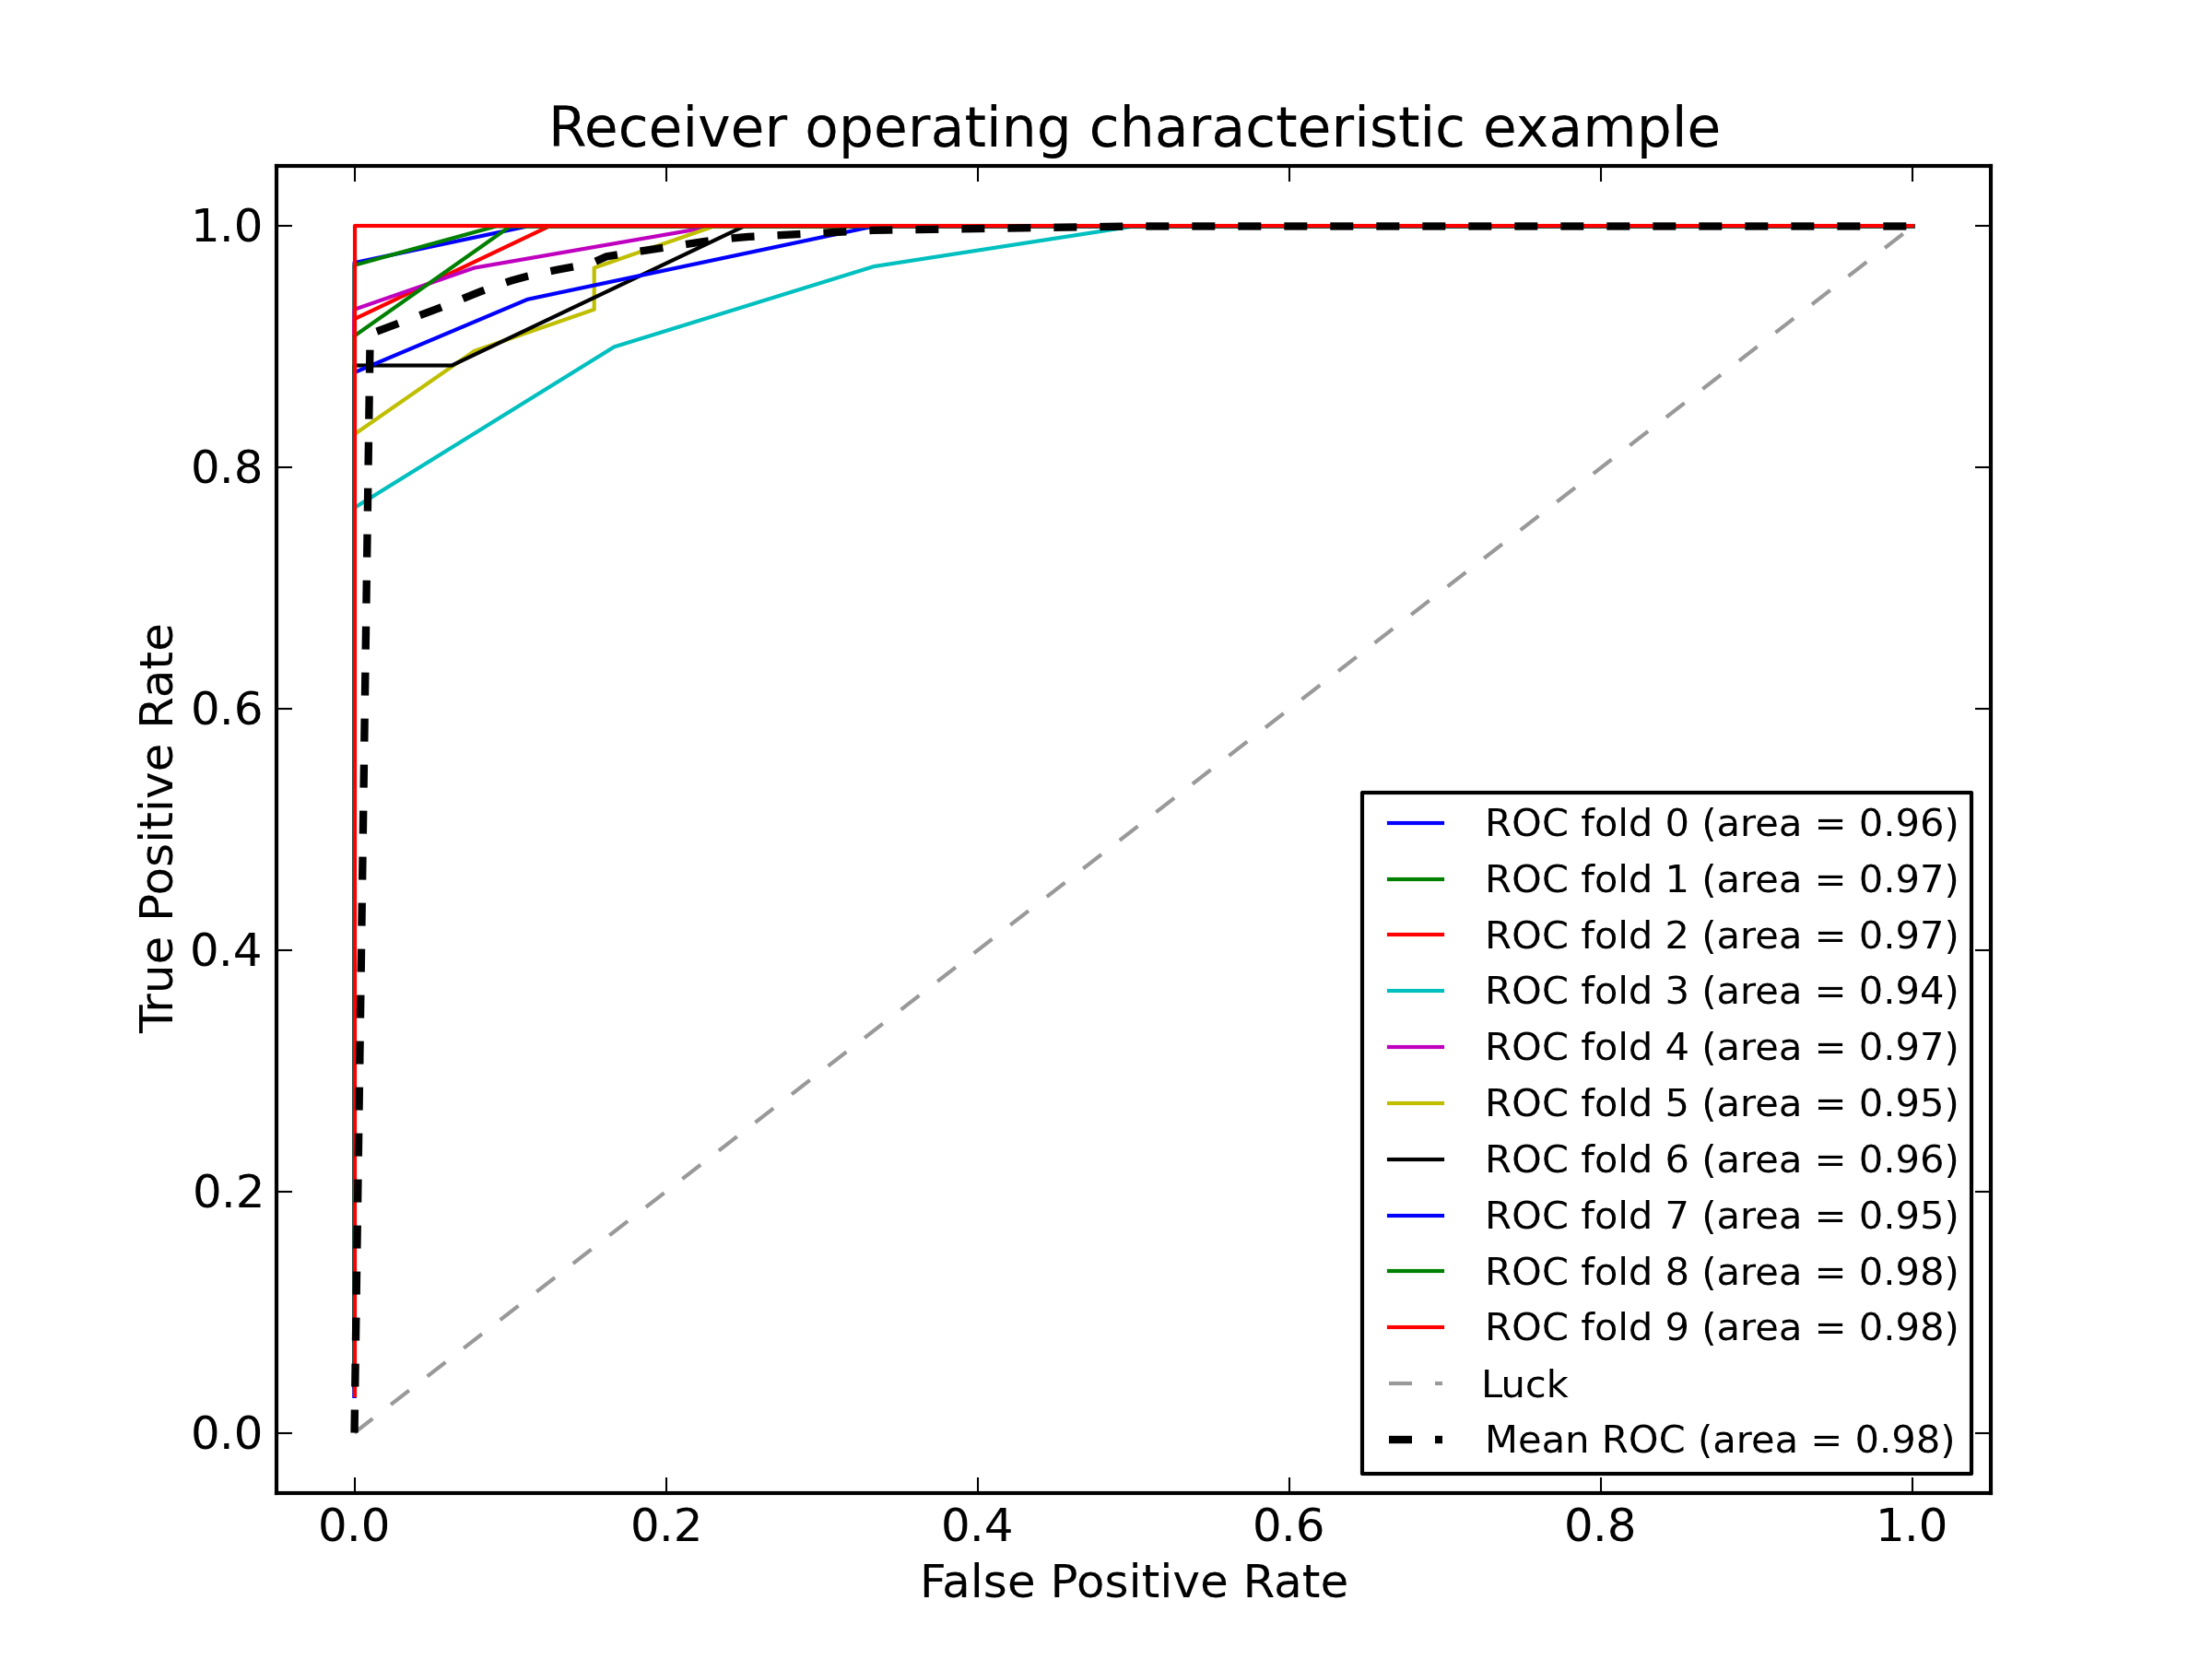
\includegraphics[width=0.36\textwidth]{pics/2_590_svm.png}}
\quad
\subfloat[Random Forests]{
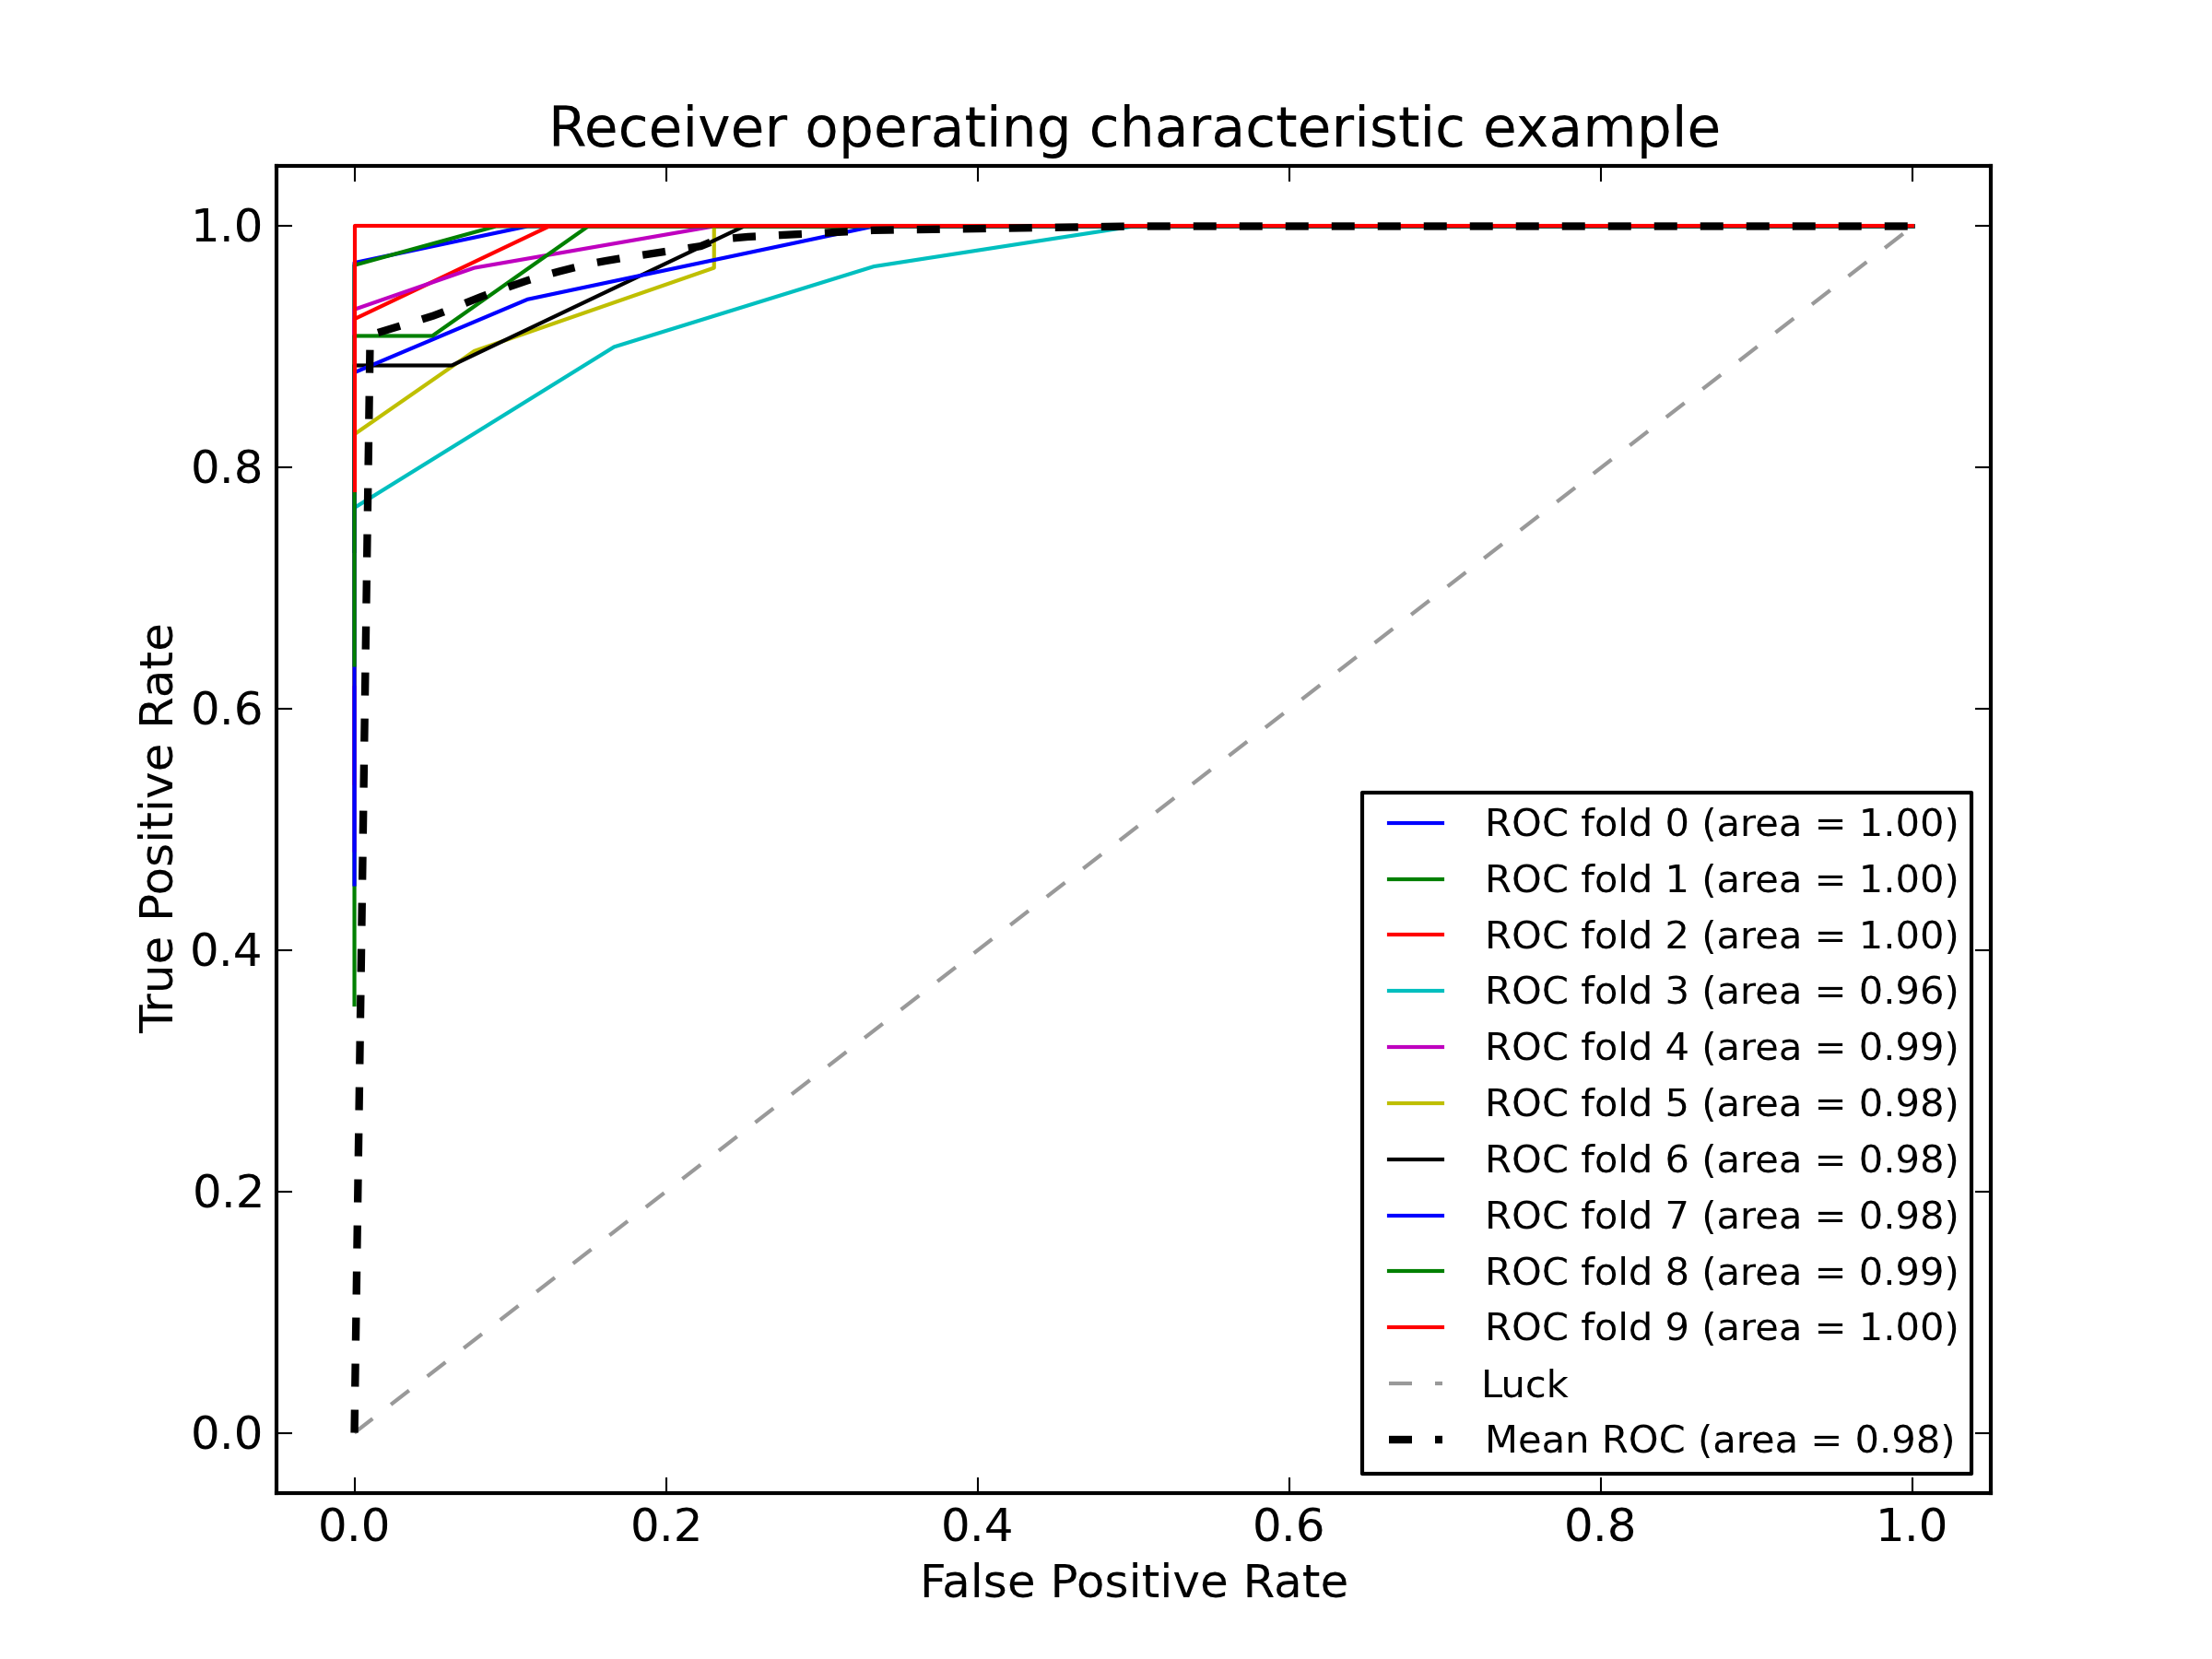
\includegraphics[width=0.36\textwidth]{pics/2_590_forest.png}}
\quad
\subfloat[Stacking - Logistic Regression]{
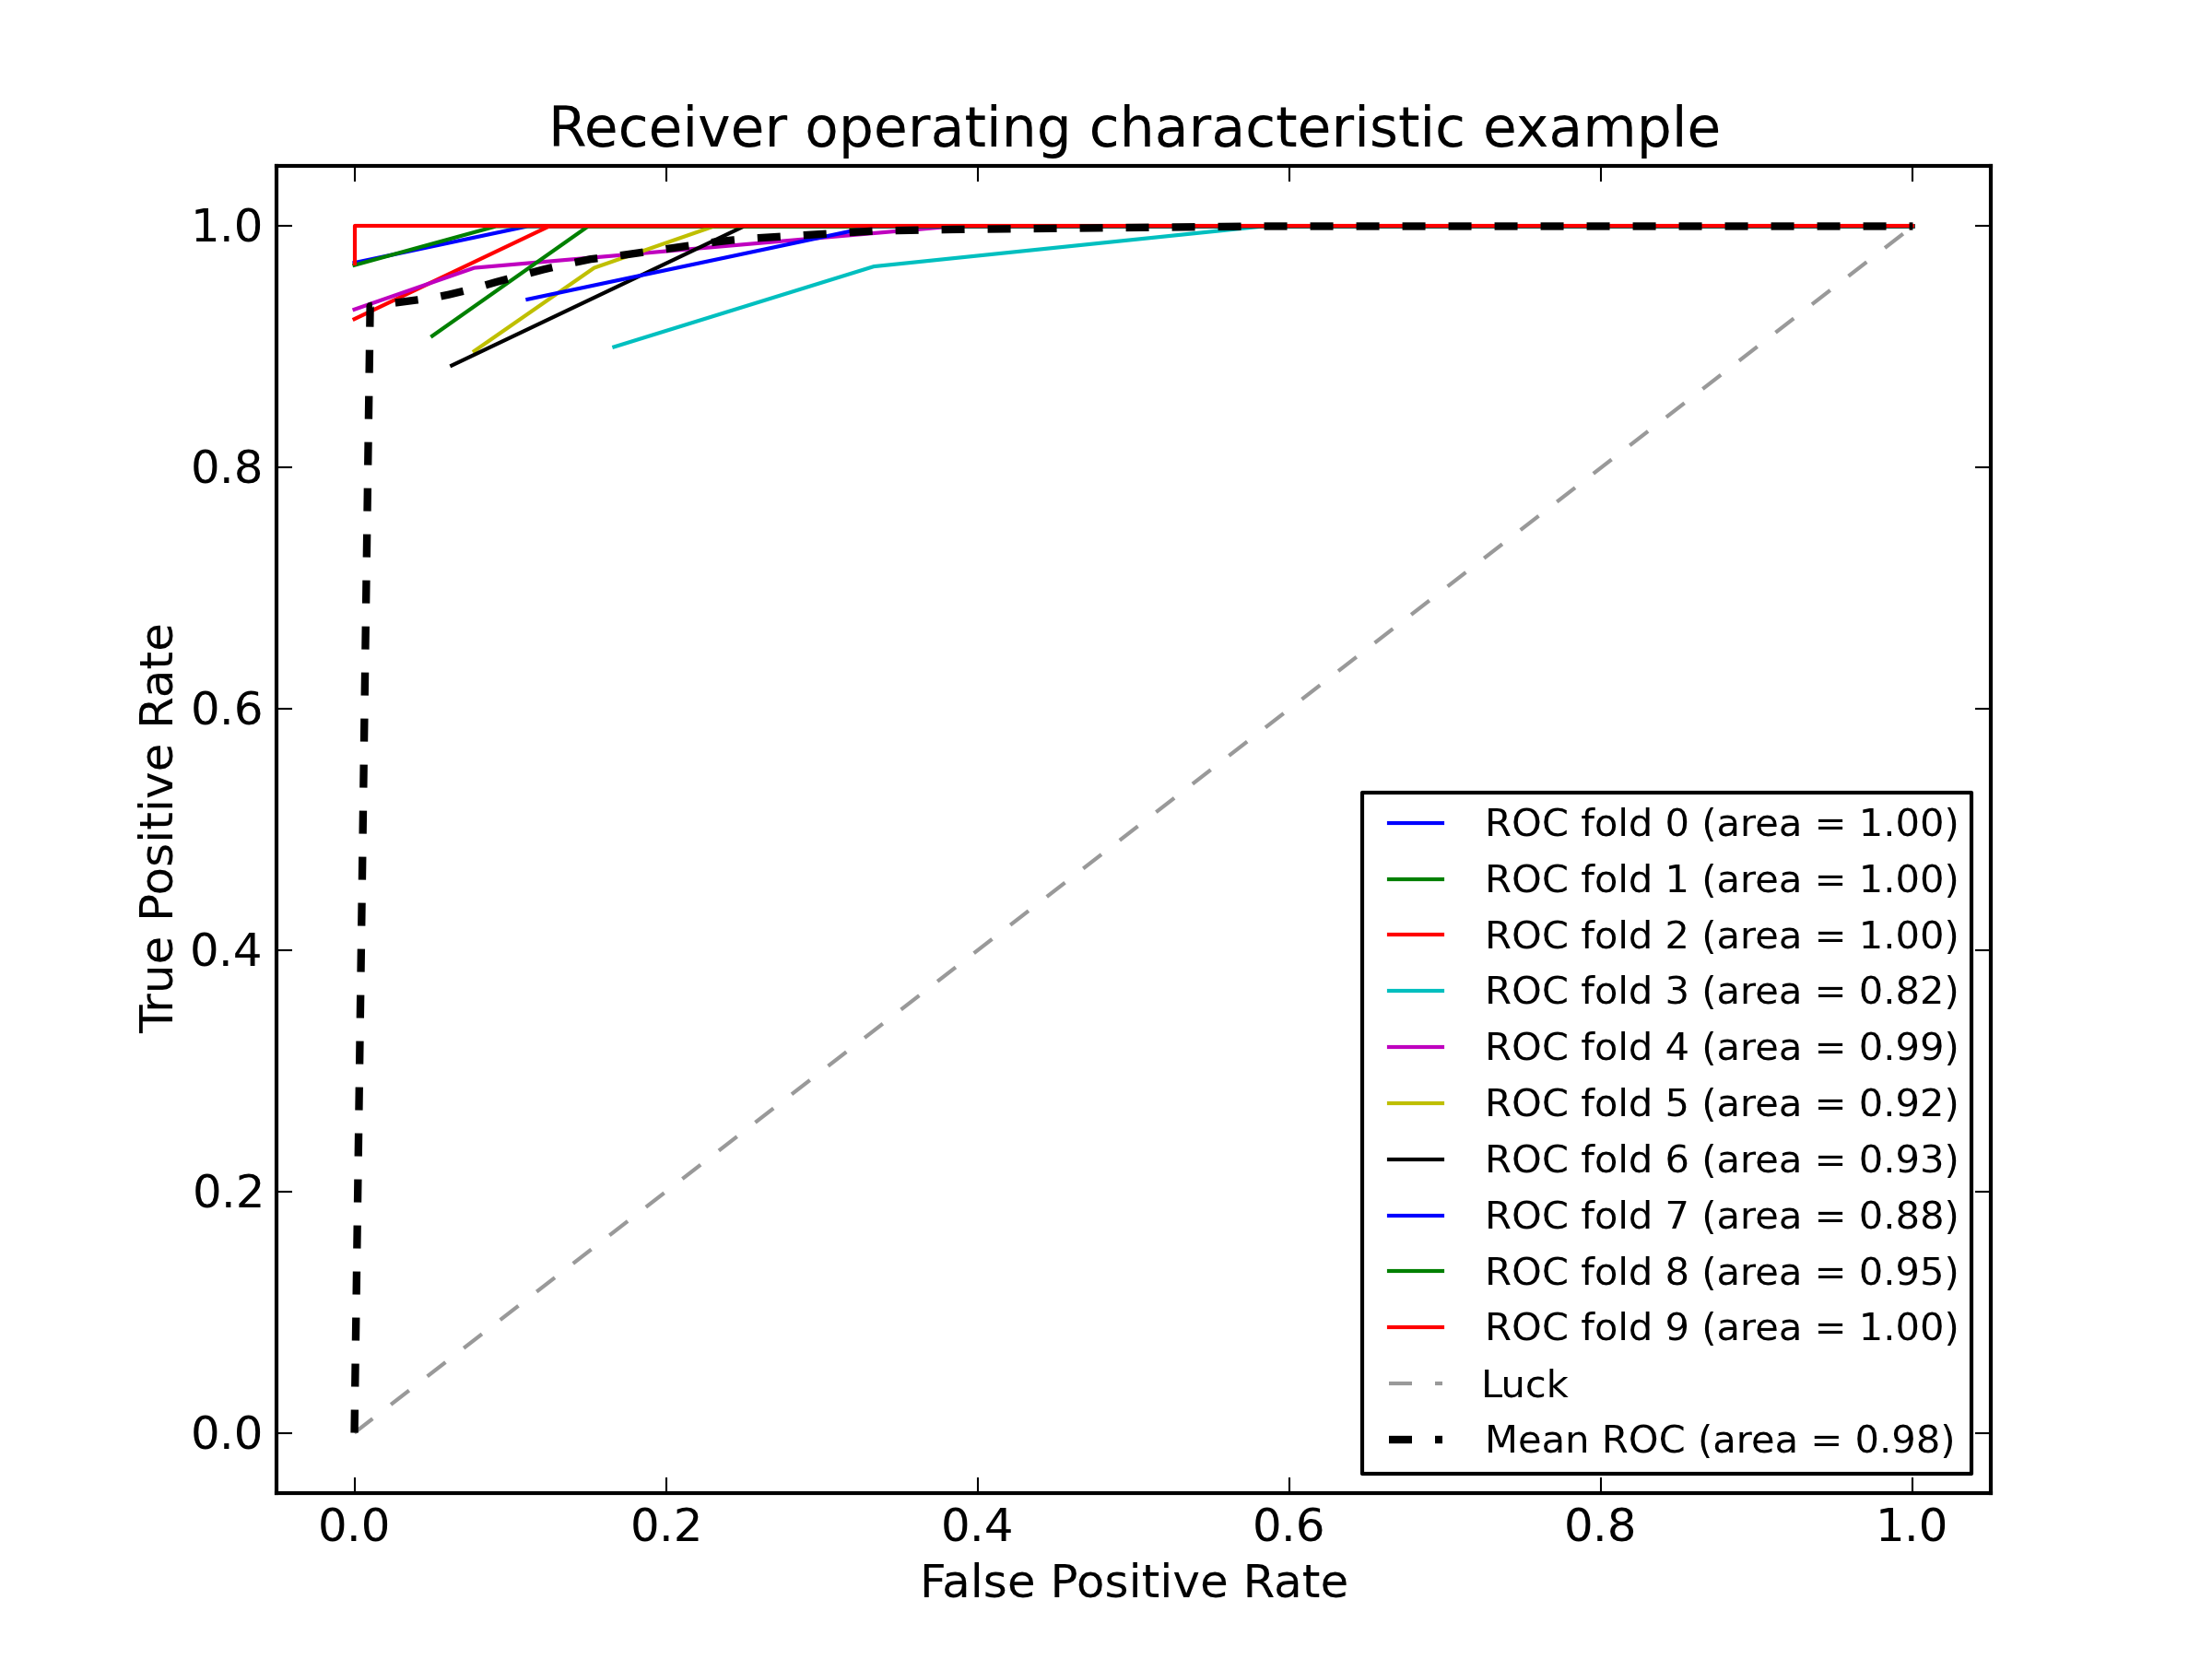
\includegraphics[width=0.36\textwidth]{pics/2_590_wmm.png}}
\quad
\subfloat[Stacking - Multi-Response Linear Models]{
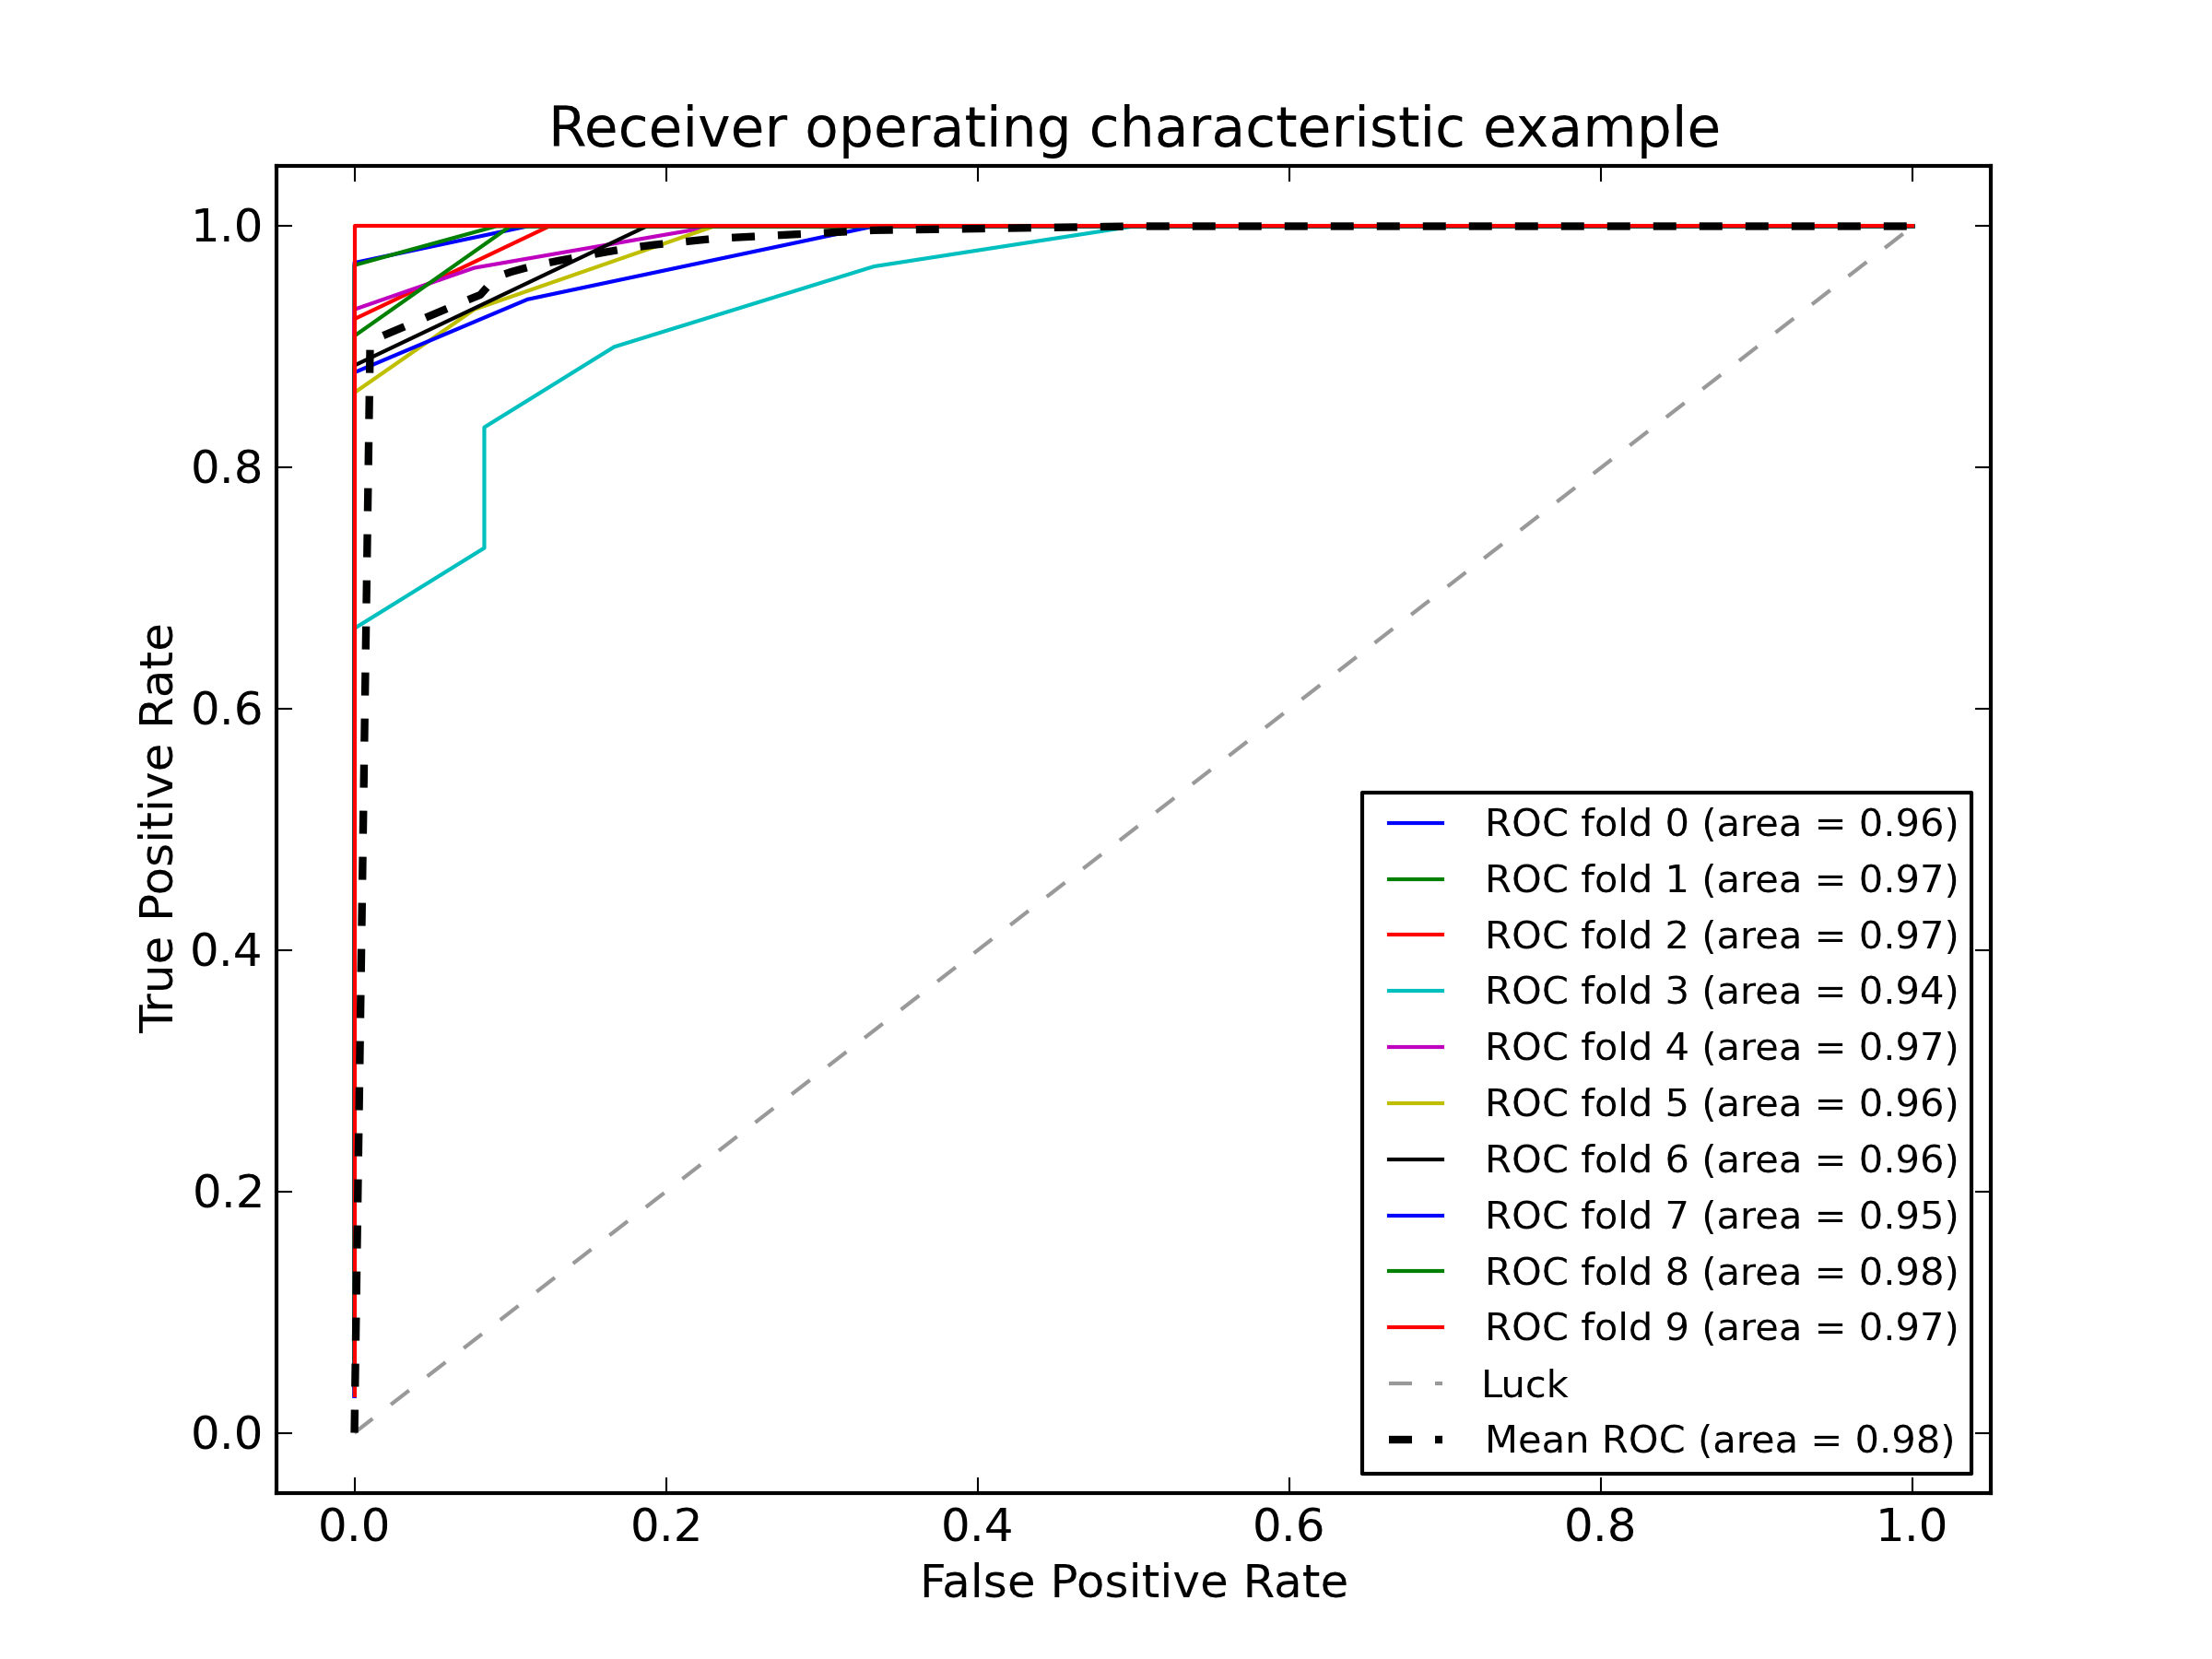
\includegraphics[width=0.36\textwidth]{pics/2_590_smm.png}}
\caption{Results for Features 1-9}
\label{fig:fig3}
\end{figure}

\section{Conclusion}
TO-DO: Allen fill this in

\end{document}
